\documentclass[9pt,openany]{extbook}
% ======================
% REQUIRED PACKAGES
% ======================
\usepackage[margin=1in]{geometry}
\usepackage{setspace}
\usepackage{graphicx}
\usepackage{amsmath,amssymb,amsfonts}
\usepackage{mathtools}
\usepackage{booktabs}
\usepackage{array}
\usepackage{multirow}
\usepackage{caption}
\usepackage{subcaption}
\usepackage{cite}
\usepackage[hidelinks]{hyperref}
\usepackage{xurl}
\setlength{\emergencystretch}{3em}
\onehalfspacing  % Change to \doublespacing if department requires strict double
\usepackage{etoolbox}
\patchcmd{\chapter}{\clearpage}{\par\vspace{2em}}{}{}
\raggedbottom
\usepackage{tikz}
\usetikzlibrary{arrows.meta, shapes.geometric, fit, backgrounds,
                positioning, calc, decorations.pathreplacing}
\usepackage{tikz-3dplot}


\usepackage{pgfplots}
\pgfplotsset{compat=1.18}
\usepackage{titlesec}
\titleformat{\chapter}[display]
  {\normalfont\large\bfseries}{\chaptertitlename\ \thechapter}{12pt}{\large}
\titlespacing*{\chapter}{0pt}{-20pt}{20pt}
\usepackage{float}
\definecolor{blueBoxLight}{HTML}{B3D4FC}
\definecolor{tealBoxLight}{HTML}{B2DFDB}
\definecolor{orangeBoxLight}{HTML}{FFE0B2}
\definecolor{greenBoxLight}{HTML}{C8E6C9}
\definecolor{grayBoxLight}{HTML}{E0E0E0}

%======================
% BEGIN DOCUMENT
% ======================
\begin{document}

% ======================
% TITLE PAGE (FORCED ONE PAGE)
% ======================
\begin{titlepage}
\thispagestyle{empty}

% Force tighter spacing ONLY on title page to prevent overflow
\begingroup
\singlespacing

\begin{center}

\vspace*{0.45in}

\textbf{
LAGENGINE: ELIMINATING LAG: A REAL-TIME PHYSICS SIMULATION\\
ENGINE WITH TEMPLATE-DRIVEN CLASSROOM AUTHORING AND\\
ADAPTIVE RL-BASED RUNTIME OPTIMISATION
}

\vspace{0.65in}

by

\vspace{0.2in}

\textbf{SATRAJIT GHOSH}

\vspace{0.55in}

A thesis submitted to the\\
Graduate School of Rutgers, The State University of New Jersey\\
in partial fulfillment of the requirements\\
for the degree of Master of Science\\
Graduate Program in Electrical and Computer Engineering

\vspace{0.65in}

Written under the direction of\\
\textbf{Dr Dov Kruger}

\vspace{0.4in}

and approved by

\vspace{0.3in}

\underline{\hspace{3.5in}}\\[0.28in]
\underline{\hspace{3.5in}}\\[0.28in]
\underline{\hspace{3.5in}}\\[0.28in]
\underline{\hspace{3.5in}}

\vfill

New Brunswick, New Jersey\\
May 2026

\end{center}

\endgroup
\end{titlepage}

\clearpage
% ======================
% ABSTRACT (Roman ii)
% ======================
\pagenumbering{roman}
\setcounter{page}{2}

\begin{center}
\textbf{ABSTRACT}
\end{center}

\vspace{1em}

Interactive physics demonstrations are widely used in science and engineering education; however, existing tools present a persistent trade-off between accessibility and performance. Full-scale game engines offer advanced rendering and physically accurate simulation but require substantial programming expertise and configuration effort, rendering them unsuitable for most classroom practitioners. Conversely, lightweight educational platforms often provide simplified interfaces at the expense of physical fidelity, extensibility, and reliable performance on heterogeneous, low-power hardware commonly found in instructional environments. This gap constrains educators who seek to deploy real-time, visually rich, and conceptually rigorous simulations without engaging in low-level engine development or manual performance tuning.

This thesis introduces \textit{LAGEngine: Eliminating Lag: A Real-Time Physics Simulation Engine with Template-Driven Classroom Authoring and Adaptive RL-Based Runtime Optimisation}, a unified C++17-based 3D engine that integrates advanced simulation, rendering, authoring, and adaptive optimisation within a single architecture. The first layer consists of a custom-built engine core featuring rigid body dynamics, XPBD-based soft body and cloth simulation, SPH fluid systems, constraint solvers, deferred physically based rendering, an Entity--Component System with JSON serialisation, Lua scripting, robotics kinematics, and a multithreaded job system with GPU-driven submission. The second layer provides an educator-facing visual editor built with Dear ImGui, offering template-driven, low-code authoring workflows that expose high-level simulation parameters while abstracting engine complexity. The third layer embeds a passive reinforcement-learning auto-tuner that observes runtime telemetry and learns cross-session configuration policies to promote stable frame times across heterogeneous classroom hardware. Together, these contributions demonstrate that template-driven authoring, a multithreaded GPU-driven low-overhead rendering runtime, and an integrated RL-based optimisation layer can be cohesively combined to enable accessible yet high-fidelity physics simulation suitable for low-power educational settings.

\clearpage

% ======================
% TABLE OF CONTENTS
% ======================
\tableofcontents
\clearpage

% ======================
% SWITCH TO ARABIC PAGE NUMBERS
% ======================
\pagenumbering{arabic}
\setcounter{page}{1}
\chapter{Introduction}

Physics education requires learners to connect symbolic formalisms such as differential equations, constraint systems, and conservation laws with observable behaviours, including oscillation, damping, collision response, and stability. While symbolic reasoning provides analytical structure, intuition often develops only when systems are visualised and their responses observed dynamically. Interactive demonstrations shorten the feedback loop between parameter adjustment and behavioural outcome, allowing learners to explore cause and effect in real time. This interaction is especially valuable for phenomena that are difficult to reproduce physically in classrooms, including complex multi-body collisions, large-scale fluid behaviour, and systematic parameter sweeps across stiffness, friction, and restitution. Interactive simulation, therefore, functions not merely as a visual aid but as an experimental medium for conceptual understanding.

Despite their pedagogical benefits, interactive demonstrations face significant production and deployment barriers. Classroom tools must be quick to create with limited preparation time, easy to modify without knowledge of the engine internals, reliable on older, resource-constrained machines, and aligned with instructional objectives. Adoption research consistently identifies limited technology resources, insufficient preparation time, and integration difficulty as primary obstacles to the use of digital simulations \cite{an2016games, kaimara2021dgbla}. Ease of use and compatibility with school hardware emerge as decisive factors in adoption decisions.

Three forms of friction commonly impede classroom deployment. Authoring friction arises when creators must understand programming languages, engine abstractions, and asset pipelines before producing a simple demonstration. Deployment friction occurs when distributing binaries, resolving driver dependencies, and handling platform differences becomes burdensome. Performance fragility occurs when a demonstration that runs smoothly on development hardware becomes unstable or stuttery on classroom machines. These constraints redirect effort from pedagogy toward engineering and discourage sustained adoption.

Prior tools have attempted to reduce programming barriers. Easy Java Simulations enabled educators to focus on mathematical models while abstracting much of the underlying engineering complexity \cite{esquembre2004ejs}.  However, classroom expectations have evolved. Educators increasingly seek real-time three-dimensional physics, modern rendering, and richer interactivity delivered reliably across heterogeneous hardware. Contemporary game engines provide these capabilities but assume developer-level expertise and modern hardware resources. AI-assisted code generation has reduced initial authoring cost by enabling rapid prototype creation from natural language descriptions \cite{benzion2025ai}, yet it does not resolve concerns related to packaging, deterministic behaviour, performance stability, or long-term maintainability. A gap, therefore, persists between educator accessibility and engine-level robustness.

This thesis addresses that gap through the design and implementation of LAGEngine, a unified real-time three-dimensional engine organised into three integrated layers. The engine core is a custom C++17 system supporting rigid body dynamics, XPBD based cloth and soft bodies, SPH fluids, constraint based joints, a deferred physically based rendering pipeline, an Entity Component System with JSON serialization, Lua scripting, skeletal animation, spatial audio, robotics based on Denavit Hartenberg kinematics and Jacobian inverse kinematics with proportional integral derivative control, and a multithreaded job system built on Chase Lev work stealing. Above this core sits an educator-facing visual editor implemented with ImGui, through which non-programmer users construct demonstrations using preset templates such as cloth with wind, projectile motion, SPH sandboxes, pendulum systems, inverse kinematics arms, and rigid body stacks, while modifying parameters through structured panels without touching engine code. The third layer is a passive reinforcement learning auto-tuner embedded within the runtime that observes telemetry, including frame time, GPU time, and job queue pressure, and applies conservative configuration adjustments between sessions to promote stable performance on low-power classroom hardware.

The core claim is that a physics demonstration platform can be both easy for non-experts to build with and viable on low-power hardware, provided you pair constrained template authoring with a performance-conscious runtime and passive metrics-driven tuning. To test this, the work asks what minimal simulation primitives cover common classroom demos, which parts of a physics-heavy frame parallelise safely, which telemetry signals yield stable adaptive behaviour, and which packaging strategies reduce deployment failures on older machines. The system contributes a teacher-first authoring workflow, a multithreaded runtime with render-graph-guided GPU submission, a passive auto-tuner with reinforcement learning as an adaptive extension, and an evaluation methodology grounded in classroom-realistic constraints. The rest of the thesis walks through architecture, implementation, and results.

\chapter{Background and Related Work}
\label{sec:background}

\subsection{Interactive Physics Education Tools}

Interactive simulations have consistently demonstrated positive effects on student engagement and conceptual understanding. The PhET project showed that carefully designed interactive environments support construction of mental models more effectively than passive instruction \cite{wieman2008phet}.Research across multiple scientific fields shows that students learn more when they can adjust simulation parameters and see the results immediately \cite{rutten2012learning}.

Authoring and deployment remain barriers. Easy Java Simulations lowered the threshold for creation by enabling educators to focus on mathematical modelling while abstracting software engineering complexity \cite{esquembre2004ejs}. This reinforced the principle that scientific intent should dominate interface design. However, EJS was developed under earlier computational expectations and largely supports two-dimensional simulations.

Teachers often struggle to adopt simulations because they lack time, resources, and easy ways to fit them into existing courses \cite{an2016games, kaimara2021dgbla}. AI tools can speed up the initial creation step \cite{benzion2025ai}, but the output is not guaranteed to run reliably, perform well, or be easy to modify later. Getting from a rough prototype to something actually deployable is still an unsolved problem.

\subsection{Physics Simulation Methods}

Real-time physics always involves a tradeoff between accuracy, stability, and speed. Mass-spring cloth models are easy to implement but blow up at high stiffness unless you use very small timesteps. Implicit integration fixes the stability problem but requires solving large linear systems every frame \cite{baraff_witkin1998}.

Position-Based Dynamics took a different approach by treating simulation as iterative constraint projection, which made it unconditionally stable even with large timesteps \cite{muller2007pbd}. The downside was that the material behaviour changed with the timestep. Extended Position-Based Dynamics fixed this by adding explicit compliance to constraints, so materials behave consistently regardless of timestep or iteration count \cite{macklin2016xpbd}.

Smoothed Particle Hydrodynamics provides a mesh-free Lagrangian approach suitable for interactive free surface flows. M\"uller et al. demonstrated interactive SPH for graphics \cite{muller2003sph}, and Ihmsen et al. surveyed subsequent refinements \cite{ihmsen2014sph}. Constraint-based rigid body contact formulations established by Baraff underpin modern sequential impulse solvers \cite{baraff1994}.

XPBD and SPH were selected for LAGEngine because they provide stable, real-time behaviour with tunable parameters that map cleanly onto adaptive control objectives.

\subsection{Real Time Rendering Architectures}

Deferred rendering stabilises cost by decoupling lighting from geometry through G Buffer storage and subsequent lighting passes \cite{gregory2018}. Physically based rendering builds on microfacet theory introduced by Cook and Torrance \cite{cook1982} and grounded in the rendering equation \cite{kajiya1986}. GGX-based shading \cite{walter2007} and image-based lighting \cite{debevec1998} enable visually consistent illumination under parameter variation.

Screen-space ambient occlusion approximates local occlusion using G-Buffer data and provides a controllable trade-off in quality \cite{kajalin2009}. Render graph architectures express frame structure as directed acyclic graphs, supporting predictable execution and resource management \cite{wihlidal2017}.

OpenGL CPU overhead can dominate performance on low-end systems. Persistent mapped buffers \cite{arb_buffer_storage}, multi draw indirect submission \cite{arb_multi_draw_indirect}, and parallel shader compilation \cite{arb_parallel_shader_compile} reduce driver cost \cite{azdo_khronos}. Because OpenGL restricts a rendering context to one thread \cite{wglMakeCurrent}, data preparation is parallelised while submission remains centralised. Explicit APIs such as Vulkan \cite{vulkan_threading_spec}, Direct3D 12 \cite{d3d12_cpu_efficiency}, and Metal \cite{metal_execution_model} allow parallel command recording but increase implementation complexity. Frame pacing is evaluated using percentile metrics and tools such as PresentMon \cite{presentmon}.

\subsection{Game Engine Architecture}
Layered engine organisation has become a practical standard because it separates concerns that would otherwise create brittle coupling between performance-critical subsystems~\cite{gregory2018}. The Entity Component System reflects a data-oriented philosophy: by grouping components of the same type in contiguous memory, iteration patterns become predictable and cache-friendly, which matters considerably on hardware where memory latency dominates compute cost. Work-stealing schedulers underpin parallel execution in most serious engines, with both strong theoretical foundations~\cite{arora1998} and well-understood practical implementations~\cite{chase_lev_2005}.

Commercial engines have converged on similar conclusions through independent paths. Unreal dedicates separate threads to simulation and rendering, recognising that coupling the two creates unpredictable frame times~\cite{ue_threaded_rendering, ue_parallel_rendering_overview}. Unity exposes job dependencies explicitly to the programmer, making parallelism a first-class authoring concern rather than an implementation detail~\cite{unity_job_dependencies, unity_jobhandle_complete}. Godot takes a more conservative approach, documenting precisely which APIs are thread-safe and requiring the developer to reason carefully about what can run concurrently~\cite{godot_thread_safe_apis}. The common thread across all three is that CPU-side work is aggressively distributed across cores, while GPU command submission is kept centralised and disciplined to avoid driver contention.
\subsection{Reinforcement Learning for System Optimisation}

Reinforcement learning has been applied to configuration tuning in systems with hardware-dependent performance characteristics. OtterTune demonstrated learned configuration recommendation for databases \cite{ottertune2017}. CDBTune and Athena extended this approach using deep reinforcement learning methods \cite{cdbtune2019, li2023athena}. These works show that learned controllers can outperform static defaults in nonlinear parameter spaces.

Engine parameters such as solver iterations and particle caps interact with workload and hardware in similarly nonlinear ways. Proximal Policy Optimisation provides stable updates \cite{ppo}, while Deep Deterministic Policy Gradient supports continuous control \cite{lillicrap2016ddpg}. Constrained Policy Optimisation and safe reinforcement learning research emphasise the explicit use of safety boundaries in real deployments \cite{cpo, safe_rl_survey}. Reproducibility concerns require multi seed evaluation and variance reporting \cite{henderson_rl_matters}.

\subsection{Synthesis and Identified Gap}

Educational research supports interactive simulations but highlights accessibility and hardware constraints as determinants of adoption \cite{wieman2008phet, rutten2012learning, an2016games, kaimara2021dgbla}. Simulation research provides stable methods such as XPBD and SPH \cite{muller2007pbd, macklin2016xpbd, muller2003sph}. Rendering and engine architecture research provide disciplined performance-oriented structures \cite{cook1982, wihlidal2017, gregory2018}. Systems research shows that learned configuration can outperform static heuristics when applied carefully \cite{ottertune2017, ppo}.

These strands remain largely disconnected in practice. Educator tools lack modern physics depth and adaptive performance, commercial engines assume developer expertise, and reinforcement learning tuners are not embedded within educator-facing simulation systems. No existing platform simultaneously integrates accessible three-dimensional authoring, a custom XPBD and SPH physics core, and a passive reinforcement learning auto-tuner for heterogeneous classroom hardware. LAGEngine is designed to satisfy these combined constraints through a unified architecture linking template-driven authoring, performance-oriented runtime design, and adaptive configuration selection.
\chapter{Problem Statement and Design Goals}

LAGEngine addresses the lack of a system that allows educators to create interactive three-dimensional physics demonstrations without engine-level programming expertise while maintaining stable performance on heterogeneous classroom hardware. Existing engines assume developer-grade skills and complex asset pipelines, whereas lightweight educational tools lack modern physics depth and performance scalability. Artificial intelligence-assisted authoring reduces prototype creation cost \cite{benzion2025ai} but does not resolve packaging, determinism, or hardware robustness. Classroom machines are frequently older and constrained, and demonstrations that perform well on development hardware may fail under real deployment conditions. Although reinforcement learning has been applied to configuration tuning in complex systems \cite{li2023athena}, it has not been integrated into educator-facing physics platforms. This work claims that accessibility and hardware-constrained performance can be addressed simultaneously through template-driven authoring, a multithreaded AZDO (Approaching Zero Driver Overhead)informed runtime, and a passive reinforcement learning auto-tuner that applies bounded adjustments between sessions.

The system must enable non programmer educators to generate, modify, and export demonstrations within minutes; execute reliably on Windows, Linux, and macOS machines including those with integrated graphics and limited resources; maintain deterministic and reproducible simulation behavior without mid session adaptation; and stabilize frame time to at least thirty frames per second on low end hardware and sixty frames per second on mid range systems. LAGEngine does not aim to compete with commercial engines in feature breadth, support networking or mobile deployment, provide film quality rendering, or perform online reinforcement learning during live sessions. This trade-off favours stability and accessibility over maximal extensibility.

\chapter{Prototype Evolution and Design Rationale}
\label{sec:prototype}

\subsection{Phase 1: Verlet Cloth Prototypes}

The first prototypes implemented cloth as a mass-spring grid, integrated with Verlet updates. A two-dimensional version simulated gravity and damping with interactive cannon impacts, while a three-dimensional extension introduced classes such as \texttt{Cloth3D}, \texttt{Particle3D}, and \texttt{Ball3D} and used iterative position projection for constraint correction. Rendering and physics were tightly coupled, and the stiffness parameters were time-step-dependent and nonphysical.

Large timesteps led to instability, and increasing stiffness only amplified divergence rather than enhancing realism. Iterative projection improved stability and reflected ideas later formalised in Position Based Dynamics \cite{muller2007pbd}, yet the absence of explicit compliance parameters limited control. These failures motivated the adoption of Extended Position Based Dynamics \cite{macklin2016xpbd}, whose timestep invariant formulation resolved the calibration and stability issues exposed by the prototype.

\subsection{Phase 2: Robosim Robotics Prototype}

The second prototype implemented a serial robot arm using Denavit Hartenberg parameters \cite{denavit1955} to describe link geometry and forward kinematics. Inverse kinematics employed a Jacobian transpose solver, and a PID controller ensured smooth actuation. All geometry was generated procedurally through simple mesh classes rather than external assets.

This work demonstrated that structured kinematic data maps cleanly onto a component-based model and that Jacobian transpose methods are sufficient for interactive demonstrations. Procedural geometry proved visually adequate without an asset pipeline, supporting an educator-focused workflow. Architectural lessons aligned with established engine design principles \cite{gregory2018} and directly informed the Robotics module of the final engine.

\subsection{Phase 3: Bullet Physics Evaluation and Rejection}

A structured exploration of Bullet Physics produced seventeen demo applications covering rigid bodies, constraints, soft bodies, and advanced features \cite{coumans2015bullet}. Although functionally rich, the API required substantial boilerplate and managed its own object lifecycle, which complicated integration with a UUID-based ECS.

The solver operated as a black box, limiting insight and tunability at the level required for adaptive auto-tuning. These constraints led to the rejection of Bullet in favour of a custom physics core. Bullet demos were retained as behavioural references, but the final system implements physics internally.

\subsection{Design Principles Derived from Prototyping}

The prototypes established four governing principles. Stability takes precedence over feature breadth because unstable simulation undermines educational value. An ECS-first architecture is essential to avoid tight coupling and ensure coherent ownership across subsystems. Solver transparency and tunability are necessary so that XPBD compliance and SPH particle counts can be exposed to the auto tuner. Procedural asset generation removes pipeline friction and keeps the engine accessible to educators. These principles define the architectural foundation of LAGEngine.

\chapter{System Architecture Overview}

\section{Architecture Overview}

LAGEngine is organized into six layers, shown in Figure~\ref{fig:system_architecture}. Each layer has a clear responsibility and communicates with adjacent layers through well-defined interfaces.

\textbf{Layer 1: Educator Authoring Layer.}
This is the top-level interface that teachers interact with. It provides a template library of preconfigured demos, a scene editor built on Dear ImGui, parameter controls for tuning simulation values, simulation presets for common setups, and an export and packaging system that serializes scenes into standalone JSON files. The editor operates directly on the same ECS scene representation used at runtime, with no intermediate abstraction in between.

\textbf{Layer 2: Application Layer (Simulation Content).}
This layer holds the actual demonstrations built using the authoring tools: physics demos, classroom experiments, robotics demos, fluid simulations, and collision experiments. These are compositions of entities and components defined in the layers below.

\textbf{Layer 3: Entity Component System (ECS).}
All simulation state lives here as typed component pools indexed by UUID-stable entities. The core components include Transform, RigidBody, Collider, MeshRenderer, Camera, Light, ScriptComponent, and AudioComponent. Every system in the runtime reads from and writes to these components.

\textbf{Layer 4: LAGEngine Runtime Core.}
This is the main execution layer, split into six subsystems. The physics engine handles collision, constraints, XPBD cloth, and SPH fluids. The rendering engine runs a deferred PBR pipeline with shadow mapping and post-processing. The multithreading subsystem provides a job scheduler with work-stealing. Scripting is handled through a Lua runtime. The robotics and animation subsystem covers skeletal animation, DH kinematics, Jacobian IK, and PID controllers. Audio runs as a separate subsystem alongside these.

\textbf{Layer 5: Adaptive RL Auto-Tuner.}
This layer sits below the runtime and observes it passively. It collects telemetry, performs frame analysis and load monitoring, runs an RL policy over aggregated metrics, and writes configuration adjustments that take effect at the next startup. It does not modify parameters during live execution, which preserves deterministic behaviour.

\textbf{Layer 6: Platform and External Libraries.}
The bottom layer handles platform abstraction. It includes OpenGL for graphics API access, GLFW for windowing, Dear ImGui for UI, math libraries, asset loading, and filesystem access.

\begin{figure}[H]
    \centering
    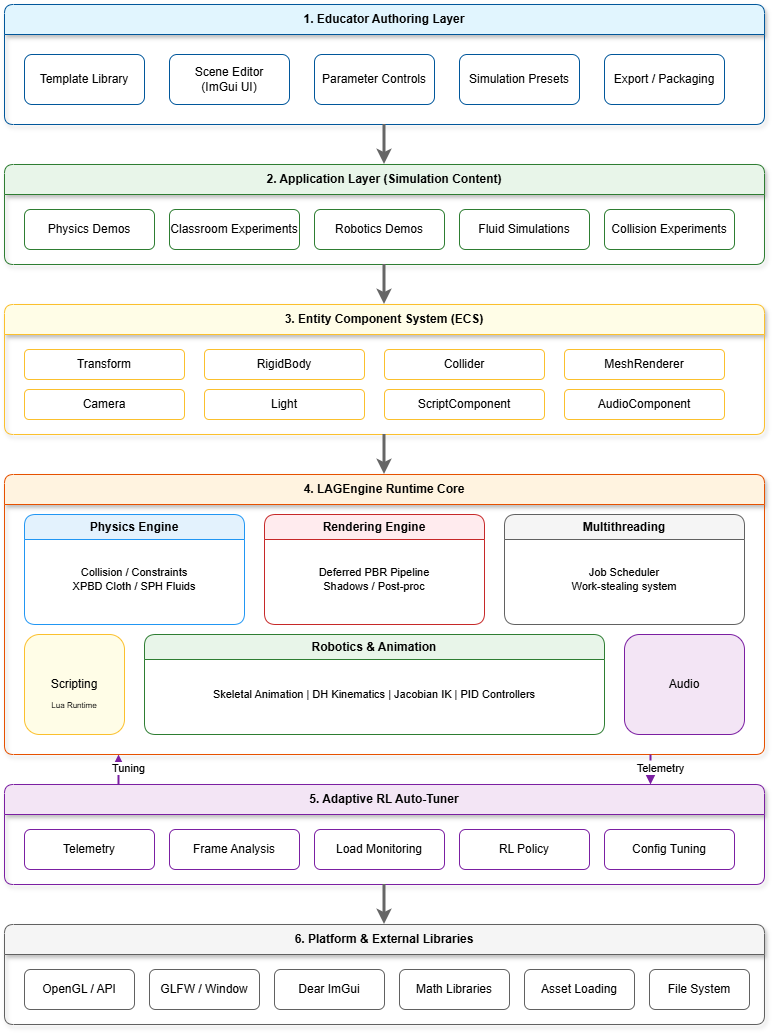
\includegraphics[height=0.5\textheight, keepaspectratio]{images/System Architecture.drawio.png}
    \caption{LAGEngine architecture showing all six layers from the educator authoring interface down to platform and external library dependencies.}
    \label{fig:system_architecture}
\end{figure}

\section{Data Flow Across Layers}

Each frame, simulation systems in Layer 4 read and write ECS components in Layer 3 (transforms, rigid bodies, XPBD constraints, SPH particles, robotics state). The rendering engine then reads the updated transforms, mesh data, and material parameters to build indirect draw buffers and submit GPU commands through the render graph.

Telemetry flows downward from Layer 4 to Layer 5. CPU frame time comes from high-resolution timers, GPU duration from timer queries, and job system statistics include queue depth, steal counts, and worker utilisation. These metrics are written into a ring buffer that retains recent history.

Between sessions, the RL module in Layer 5 reads aggregated telemetry through a pybind11 bridge, builds a state vector from exponentially weighted moving averages, and runs policy inference to produce candidate configurations (solver iterations, resolution scale, shadow quality, batching thresholds). Safety gates validate the output before writing a config file that Layer 4 consumes on the next startup.

Tuning flows upward from Layer 5 back into Layer 4, while telemetry flows downward from Layer 4 into Layer 5, forming a closed feedback loop across sessions.

\section{Deployment Model}

The engine core is compiled as a static C++17 library. The editor and example applications link directly against this library, ensuring identical runtime behaviour between development and exported builds. Scene state is serialised into JSON using UUID-stable references, and assets are packaged into a self-contained archive.

Export produces a standalone executable bundle containing the engine binary, scene description, shaders, and required assets. No external installation steps are required beyond execution of the binary. The platform abstraction layer supports Windows, Linux, and macOS using OpenGL 4.x, enabling compatibility with integrated GPUs and older classroom hardware.




\usetikzlibrary{arrows.meta, shapes.geometric, fit, backgrounds,
                positioning, calc, decorations.pathreplacing}

% ── Colour palette ──────────────────────────────────────────────────────────
\definecolor{blueBox}{RGB}{30,70,120}
\definecolor{tealBox}{RGB}{20,90,90}
\definecolor{orangeBox}{RGB}{180,80,20}
\definecolor{greenBox}{RGB}{30,100,50}
\definecolor{grayBox}{RGB}{60,60,80}
\definecolor{bgDark}{RGB}{18,18,35}
\definecolor{textLight}{RGB}{220,220,230}
\definecolor{arrowCol}{RGB}{100,180,220}

% ── Shared TikZ style ────────────────────────────────────────────────────────
\tikzset{
  block/.style  = {rectangle, rounded corners=4pt,
                   minimum width=#1, minimum height=0.7cm,
                   text centered,align=center, font=\small\sffamily,
                   text=textLight, draw=arrowCol, line width=0.6pt},
  block/.default = 3.2cm,
  sblock/.style = {block=2.4cm},
  arr/.style    = {-{Stealth[length=5pt]}, arrowCol, line width=0.8pt},
  darr/.style   = {arr, dashed},
  lbl/.style    = {font=\small\sffamily\bfseries, text=black},,
  grp/.style    = {rounded corners=6pt, draw=#1, line width=1pt,
                   fill=#1!10, fill opacity=0.25, inner sep=6pt},
}

% ═══════════════════════════════════════════════════════════════════════════════
\chapter{Engine Core Implementation}
% ═══════════════════════════════════════════════════════════════════════════════

\section{Physics Engine}

The rigid body subsystem handles the motion and rotation of objects. Each frame, forces and torques are accumulated in each body's component data from the subsystems that apply them (gravity, springs, user input, etc.). Once all forces are collected, a semi-implicit Euler integrator updates linear and angular velocities first, then advances position and orientation. Inertia tensors are stored in body-local space and rotated into world space at every frame, so that rotational responses remain physically correct as objects tumble. The key design choice here is that force accumulation and integration are separate steps. Any subsystem can write forces into component data without needing to know how integration works, keeping the code decoupled.

Collision detection runs in two stages. The broad phase uses a spatial hash that divides world space into fixed-size grid cells. Each object is inserted into whichever cells it overlaps. To find potential collisions, the system only checks objects that share a cell, reducing the cost from a naive $O(n^2)$ pairwise check to roughly $O(n)$ in practice. The cell size is chosen to match the typical object diameter so most objects land in one or two cells.

Pairs that survive the broad phase move into narrow-phase testing. The engine supports six shape-pair combinations: box versus box, sphere versus sphere, box versus sphere, capsule versus capsule, and plane interactions with the other shapes. Each narrow-phase test produces a contact manifold, a small data structure that stores the penetration depth (how far the objects overlap), the contact normal (the direction to push them apart), and one or more contact points on the surface.

Contact manifolds are then fed into a sequential-impulse solver based on the Gauss-Seidel method, consistent with constraint-based formulations~\cite{baraff1994}. The solver iterates over all contacts multiple times per frame. On each pass, it computes impulses that push overlapping objects apart along the contact normal (non-penetration), resist sliding along the contact surface (friction), and applies both velocity-level and positional corrections. The positional correction step is important because velocity-only solving allows small amounts of drift to accumulate over time, eventually causing objects to visibly sink into each other.

Joint constraints (distance, fixed, hinge, and slider) are solved in the same iterative loop alongside contacts. Distance joints keep two anchor points at a fixed separation. Fixed joints lock relative position and orientation entirely. Hinge joints allow rotation around a single axis. Slider joints allow translation along a single axis. Treating joints and contacts uniformly in one solver pass means they naturally interact with each other without special-case code.

% ── Figure: Collision pipeline ───────────────────────────────────────────────
\begin{figure}[h]
\centering
\begin{tikzpicture}[node distance=0.55cm]
  \node[block=3.6cm, fill=blueBox]  (sp)  {Spatial Hash\\Broad Phase};
  \node[block=3.6cm, fill=blueBox, below=of sp]  (np) {Narrow Phase\\(per shape pair)};
  \node[block=3.6cm, fill=tealBox,  below=of np] (cm) {Contact Manifold\\(depth, normal, pts)};
  \node[block=3.6cm, fill=greenBox, below=of cm] (si) {Sequential Impulse\\Solver (GS)};
  \node[block=3.6cm, fill=grayBox,  below=of si] (jt) {Joint Constraints\\(distance/hinge/slider)};

  \draw[arr] (sp) -- (np)  node[midway,right,lbl]{candidate pairs};
  \draw[arr] (np) -- (cm)  node[midway,right,lbl]{contact data};
  \draw[arr] (cm) -- (si)  node[midway,right,lbl]{manifolds};
  \draw[arr] (si) -- (jt)  node[midway,right,lbl]{velocity + pos correction};

  % side labels
  \node[lbl, left=0.6cm of sp]  {$O(n)$ cells};
  \node[lbl, left=0.6cm of np]  {6 shape pairs};
  \node[lbl, left=0.6cm of si]  {iterative};
\end{tikzpicture}
\caption{Collision detection and resolution pipeline.}
\label{fig:collision_pipeline}
\end{figure}

% ─────────────────────────────────────────────────────────────────────────────
\section{XPBD Soft Body and Cloth}

Extended Position-Based Dynamics (XPBD) improves on standard PBD by adding an explicit compliance parameter to each constraint~\cite{muller2007pbd,macklin2016xpbd}. Compliance controls how stiff or soft a constraint is. The important property is that stiffness stays consistent regardless of the timestep or how many solver iterations you run. In standard PBD, cutting the iteration count makes materials feel softer, which is a problem. In XPBD, cutting iterations degrades quality gracefully but the material still behaves like the same material. This is what makes XPBD a good fit for the auto-tuner: when the system detects that hardware is struggling, it can reduce solver iterations to save time without changing how the cloth or soft body feels to the user.

The solver loop works as follows. First, every particle's position is predicted forward using its current velocity: $\tilde{x} = x + \Delta t\,v$. These predicted positions are then iteratively corrected by projecting three types of constraints. Distance constraints keep connected particles at their rest-length separation, preventing cloth from stretching unrealistically. Bending constraints resist folding between adjacent triangles, controlling how stiff or floppy the material looks. Volume constraints maintain the overall volume of soft bodies to prevent collapse under pressure.

Each constraint projection computes a Lagrange multiplier update $\Delta\lambda$, which determines how far each affected particle should move. This update is scaled by the constraint's compliance value $\alpha$ and the timestep $\Delta t$. Low compliance means stiff behaviour (the constraint is enforced tightly), high compliance means soft behaviour (the constraint allows more stretch). The projection and multiplier update steps repeat for a configurable number of iterations. More iterations produce more accurate results but cost more time.

After all iterations finish, velocities are reconstructed from the difference between the corrected positions and the original positions: $v \leftarrow (\tilde{x} - x) / \Delta t$. Deriving velocities from position changes rather than tracking them independently ensures that momentum stays consistent with where particles actually ended up.

Two additional features sit atop this loop. Cloth tearing checks each distance constraint after solving and deletes any constraint whose stretch ratio exceeds a configurable threshold $\tau$. Once deleted, the particles on either side are no longer connected, which creates a visible rip in the mesh. Self-collision is handled by an \texttt{OctreeAccelerator} that spatially partitions particles into a tree structure. Instead of testing every particle against every other particle, the narrow-phase self-collision tests only run between particles that occupy nearby tree nodes, keeping the cost manageable as particle counts grow.

% ── Figure: XPBD loop ────────────────────────────────────────────────────────
\begin{figure}[H]
\centering
\begin{tikzpicture}[node distance=0.55cm]
  \node[block=4.0cm, fill=blueBox]  (pred) {Predict positions\\$\tilde{x} = x + \Delta t\,v$};
  \node[block=4.0cm, fill=tealBox,  below=of pred] (proj) {Project constraints\\(distance / bend / vol)};
  \node[block=4.0cm, fill=tealBox,  below=of proj] (lam)  {Update multipliers\\$\Delta\lambda$ with compliance $\alpha$};
  \node[block=4.0cm, fill=greenBox, below=of lam]  (vel)  {Reconstruct velocities\\$v \leftarrow (\tilde{x}-x)/\Delta t$};
  \node[block=4.0cm, fill=orangeBox,below=of vel]  (tear) {Tear check\\delete if stretch $> \tau$};

  \draw[arr] (pred) -- (proj);
  \draw[arr] (proj) -- (lam);
  \draw[arr] (lam)  -- (vel);
  \draw[arr] (vel)  -- (tear);
  % iteration back-arrow
  \draw[arr] (lam.east) -- ++(0.5,0) |- (proj.east)
        node[midway, right, lbl]{iterate $n$ times};
\end{tikzpicture}
\caption{XPBD constraint projection loop.}
\label{fig:xpbd_pipeline}
\end{figure}

% ─────────────────────────────────────────────────────────────────────────────
\section{SPH Fluid Simulation}

Fluid simulation uses Smoothed Particle Hydrodynamics (SPH), a meshfree method where the fluid is represented as a collection of particles rather than a fixed grid~\cite{muller2003sph,ihmsen2014sph}. Each particle carries mass, position, velocity, and density. The behaviour of the fluid emerges from how these particles interact with their neighbours.

The simulation runs in four stages each frame. The first stage finds neighbours. Each particle only interacts with other particles within a small radius $h$ called the smoothing length. To avoid checking every particle against every other particle, the system reuses the same spatial hash grid used by the rigid body collision system. Particles are inserted into grid cells based on their position, and neighbour queries only look at adjacent cells. This also means the job system can split density and force calculations across worker threads in parallel, since the spatial hash is already shared infrastructure.

The second stage estimates density. Each particle's density $\rho_i$ is computed by summing weighted contributions from all neighbours using the poly6 kernel function. Particles in crowded regions end up with high density, particles in sparse regions end up with low density. Getting density right is critical because every other force depends on it.

The third stage computes forces. Pressure forces push particles apart when local density exceeds the rest density $\rho_0$. Pressure is computed from a simple equation of state:
\[
  p_i = k\,(\rho_i - \rho_0),
\]
where $k$ is a stiffness constant that controls how strongly the fluid resists compression. The gradient of the pressure field is evaluated using the spiky kernel, which has a sharp peak at close range and produces the repulsive forces that keep particles from collapsing into each other. Viscosity forces resist relative motion between neighbouring particles, making the fluid flow smoothly rather than behaving like a collection of independent particles. These are computed using a Laplacian kernel. Surface tension is handled through additional force terms that pull surface particles inward, and boundary conditions are enforced by applying response forces when particles collide with static geometry.

The fourth stage integrates. All accumulated forces are applied using the same semi-implicit Euler integrator used by the rigid body system. Velocities are updated first from forces, then positions are advanced from the updated velocities.

For rendering, the engine does not try to build a triangle mesh from the particles. Instead, a screen-space fluid renderer takes the particle positions, renders them as depth values, smooths the depth buffer to remove individual particle shapes, reconstructs surface normals from the smoothed depth, and then shades the result through the deferred physically based rendering pipeline. This produces a continuous fluid surface without the cost of explicit mesh reconstruction.

% ── Figure: SPH pipeline ─────────────────────────────────────────────────────
\begin{figure}[H]
\centering
\begin{tikzpicture}[node distance=0.55cm]
  \node[block=3.8cm, fill=blueBox]  (ns) {Spatial Hash\\Neighbour Search};
  \node[block=3.8cm, fill=tealBox,  below=of ns] (de) {Density Estimation\\poly6 kernel};
  \node[block=3.8cm, fill=tealBox,  below=of de] (fc) {Force Computation\\spiky + viscosity kernels};
  \node[block=3.8cm, fill=greenBox, below=of fc] (in) {Semi-implicit Euler\\Integration};
  \node[block=3.8cm, fill=grayBox,  below=of in] (ss) {Screen-Space\\Fluid Renderer};

  \draw[arr] (ns) -- (de);
  \draw[arr] (de) -- (fc);
  \draw[arr] (fc) -- (in);
  \draw[arr] (in) -- (ss);
  \node[lbl, right=0.5cm of de] {$\rho_i = \sum_j m_j W(\mathbf{r},h)$};
  \node[lbl, right=0.5cm of fc] {$\mathbf{f}^p,\,\mathbf{f}^\nu$};
\end{tikzpicture}
\caption{SPH simulation pipeline.}
\label{fig:sph_pipeline}
\end{figure}

% ─────────────────────────────────────────────────────────────────────────────
\section{Rendering Pipeline}

\section{Rendering Pipeline}

The engine uses a deferred rendering pipeline, which means geometry and lighting are handled in separate passes rather than all at once. This separation is important because it makes the cost of lighting independent of how much geometry is in the scene, which keeps frame times stable even when the physics simulation is pushing a lot of objects.

The first pass is the geometry pass. Every visible object is drawn once, and instead of computing final pixel colours, the pipeline writes surface information into a set of textures called the G-Buffer. These textures store world-space position (RGB32F), surface normals (RGB16F), albedo colour and roughness (RGBA8), metallic and ambient occlusion values (RG8), and depth (D24S8). After this pass, the GPU has a complete description of every visible surface without having processed any lights yet.

The lighting pass reads from the G-Buffer and computes final shading for each pixel. The shading model is Cook-Torrance, a physically based BRDF that combines three terms~\cite{cook1982,walter2007,kajiya1986}. The GGX normal distribution function controls how tight or spread out specular highlights are based on surface roughness. Smith-GGX geometric shadowing accounts for microfacet self-occlusion at glancing angles. Fresnel-Schlick reflectance controls how much light reflects versus enters the surface depending on viewing angle. Together these three terms produce materials that respond to light in a physically plausible way.

For indirect lighting, the engine uses image-based lighting with preintegrated environment maps~\cite{debevec1998}. An environment map is pre-convolved at multiple roughness levels so that looking up indirect specular reflections at runtime is a single texture sample rather than an expensive integration.

Shadows come from two sources. Directional lights (like sunlight) use cascaded shadow maps, which split the view frustum into distance-based slices with progressively lower resolution farther from the camera. Point lights use omnidirectional cube-map shadows, rendering the scene into six faces of a cube map from the light's position.

Screen-space ambient occlusion adds contact shadows in corners and crevices where ambient light would be partially blocked~\cite{kajalin2009}. It works by sampling a hemisphere of points around each pixel in view space, testing how many of those samples fall inside nearby geometry, and then applying a separable blur pass to smooth the result.

% ── Figure: Deferred pipeline ────────────────────────────────────────────────
\begin{figure}[H]
\centering
\begin{tikzpicture}[node distance=0.45cm and 0.3cm]
  % passes left to right
  \node[block=2.8cm, fill=blueBox]  (geo)  {Geometry Pass};
  \node[block=2.6cm, fill=blueBox,  right=0.4cm of geo]  (gb)   {G-Buffer\\pos/nrm/alb/met/dep};
  \node[block=2.6cm, fill=orangeBox,right=0.4cm of gb]   (shd)  {Shadow Pass\\CSM + CubeMap};
  \node[block=2.6cm, fill=tealBox,  right=0.4cm of shd]  (lgt)  {Lighting Pass\\Cook-Torrance BRDF};
  \node[block=2.6cm, fill=greenBox, below=0.9cm of lgt]  (ssao) {SSAO\\hemisphere + blur};
  \node[block=2.6cm, fill=grayBox,  below=0.9cm of shd]  (ibl)  {IBL\\env map};
  \node[block=2.6cm, fill=grayBox,  below=0.9cm of gb]   (post) {Post-Process\\tonemap + FXAA};
  \node[block=2.6cm, fill=greenBox, below=0.9cm of geo]  (out)  {Framebuffer\\Output};

  \draw[arr] (geo)  -- (gb);
  \draw[arr] (gb)   -- (shd);
  \draw[arr] (shd)  -- (lgt);
  \draw[arr] (lgt)  -- (ssao);
  \draw[arr] (ssao.west) -- (ibl.east);
  \draw[arr] (ibl.west)  -- (post.east);
  \draw[arr] (post.west) -- (out.east);
  \draw[darr](gb.south)  -- (post.north);
\end{tikzpicture}
\caption{Deferred rendering pipeline pass sequence.}
\label{fig:deferred_pipeline}
\end{figure}

% ─────────────────────────────────────────────────────────────────────────────
\section{Render Graph and GPU Submission}

The render graph organises each frame as a directed acyclic graph of render pass nodes~\cite{wihlidal2017}. Each node declares what render targets it reads from and what render targets it writes to. The graph resolves dependencies automatically and executes passes in topological order. This means nobody has to manually manage framebuffer binding order or figure out which pass needs to run before which. It also enables the system to reuse GPU memory across passes that do not overlap, since the graph knows exactly when each resource is live.

GPU submission is designed around the Approaching Zero Driver Overhead (AZDO) philosophy~\cite{azdo_khronos}, which minimises the per-frame cost of talking to the graphics driver.

The first technique is persistent mapped buffers. Instead of mapping and unmapping GPU buffers every frame to upload instance data (transforms, material indices, etc.), the engine allocates ring buffers once using \texttt{GL\_ARB\_buffer\_storage} and keeps them mapped for the lifetime of the application~\cite{arb_buffer_storage}. Each frame writes to the next section of the ring, avoiding the overhead of repeated map and unmap calls.

The second technique is indirect drawing. Rather than issuing one draw call per object, the engine packs draw parameters (vertex count, instance count, buffer offsets) into an indirect command buffer and issues a single \texttt{MultiDrawIndirect} call that processes all of them at once~\cite{arb_multi_draw_indirect}. This amortises the driver validation cost that normally happens per draw call.

The third technique is asynchronous shader compilation. Shaders are compiled in the background using \texttt{GL\_ARB\_parallel\_shader\_compile}, which eliminates the stalls that normally happen the first time a new shader is used.

Threading follows OpenGL's context ownership rules. OpenGL contexts can only be current on one thread at a time (\texttt{wglMakeCurrent} exclusivity~\cite{wglMakeCurrent}), so a dedicated submission thread holds the context and issues all GPU commands. Worker threads run in parallel preparing indirect command buffers, building instance data streams, and performing culling. Once the data is ready, the submission thread picks it up and sends it to the GPU.

% ── Figure: Render graph DAG ─────────────────────────────────────────────────
\begin{figure}[H]
\centering
\begin{tikzpicture}[node distance=0.5cm and 1.0cm]
  \node[sblock, fill=blueBox]  (geo)  {GeometryPass};
  \node[sblock, fill=orangeBox, right=1.2cm of geo] (csm)  {CSMPass};
  \node[sblock, fill=orangeBox, below=of csm]       (cube) {CubeMapPass};
  \node[sblock, fill=tealBox,   right=1.2cm of csm] (lgt)  {LightingPass};
  \node[sblock, fill=greenBox,  right=1.2cm of lgt] (ssao) {SSAOPass};
  \node[sblock, fill=grayBox,   below=of ssao]      (post) {PostProcess};
  \node[sblock, fill=greenBox,  right=1.2cm of ssao](out)  {Output};
  \draw[arr] (geo)  -- (csm);
  \draw[arr] (geo)  -- (cube);
  \draw[arr] (geo.north) -- ++(0,0.5) -| (lgt.north);
  \draw[arr] (csm)  -- (lgt);
  \draw[arr] (cube) -- (lgt);
  \draw[arr] (lgt)  -- (ssao);
  \draw[arr] (lgt)  -- (post);
  \draw[arr] (ssao) -- (out);
  \draw[arr] (post) -- (out);
  \node[lbl, below=0.15cm of geo] {GBuffer write};
  \node[lbl, below=0.15cm of lgt] {GBuffer read};
\end{tikzpicture}
\caption{Render graph directed acyclic graph showing pass dependencies.}
\label{fig:render_graph}
\end{figure}
% ─────────────────────────────────────────────────────────────────────────────
\section{Engine Systems}

The Entity Component System assigns every entity a 64-bit UUID and stores component data in typed pools. The system supports over twenty component types covering physics, rendering, scripting, audio, animation, and robotics. UUIDs remain stable across serialisation, so references between entities survive save and load cycles. Scenes serialise to JSON using \texttt{nlohmann/json}, and the prefab system supports deep-copy instantiation so that duplicating a complex entity hierarchy copies all of its components and child references correctly.

Scripting uses Lua 5.4 and exposes three callbacks: \texttt{OnStart} runs once when an entity is created, \texttt{OnUpdate} runs every frame, and \texttt{OnCollision} fires when the physics system detects a contact involving that entity. A file watcher monitors script files on disk and hot-reloads them when they change, so teachers can edit behaviour without restarting the engine.

Asset management is split across three systems. ResourceManager handles loading and caching of raw assets (textures, meshes, shaders). AssetDatabase tracks metadata and provides lookup by name or UUID. PresetManager stores reusable configuration bundles that can be applied to entities or components.

Skeletal animation interpolates between keyframes using SLERP for rotations and linear interpolation for positions. Skinning matrices are computed and uploaded to the GPU every frame so that mesh vertices deform to follow the skeleton.

Spatial audio uses OpenAL and reads world positions directly from each entity's TransformComponent every frame. As objects move in the simulation, their sound sources move with them automatically.

The robotics subsystem models articulated arms using Denavit-Hartenberg parameterisation~\cite{denavit1955}, which defines each joint as a sequence of rotations and translations along standardised axes. Inverse kinematics uses the Jacobian-transpose method~\cite{buss2004ik} to compute joint angles that move the end effector toward a target position. Joint motors are driven by discrete PID controllers stored in RobotArmComponent, which compute corrective torques from the error between desired and actual joint angles each frame.

% ─────────────────────────────────────────────────────────────────────────────
\section{Job System and Parallel Execution}

The job system distributes work across all available CPU cores using a work-stealing architecture~\cite{chase_lev_2005,arora1998}. Each worker thread owns a private double-ended queue (deque). When a thread finishes its own work, it steals tasks from the back of another thread's deque. This keeps all cores busy without requiring a central task queue that would become a contention bottleneck.

The main thread handles three responsibilities that cannot be parallelised: processing input events, updating the Dear ImGui interface, and submitting GPU commands (since the OpenGL context is bound to this thread). Everything else runs on workers.

Worker tasks include physics integration and constraint solving, XPBD soft-body projection, SPH fluid computation, inverse kinematics for robotic arms, transform hierarchy propagation, broad-phase spatial hash updates, frustum culling, instance data stream construction, and indirect draw buffer population. These tasks are structured as a dependency graph: physics must finish before IK runs, IK must finish before culling, and culling must finish before indirect buffers are built. Once the buffers are ready, the main thread picks them up and submits them to the GPU.

This decomposition follows established multi-threaded engine patterns~\cite{ue_threaded_rendering} and respects the constraint that only one thread can own the OpenGL context at a time, while still keeping worker threads saturated with useful computation every frame.

% ── Figure: Per-frame job graph ───────────────────────────────────────────────
\begin{figure}[H]
\centering
\begin{tikzpicture}[node distance=0.5cm and 0.6cm]
  % Main thread column
  \node[block=3.0cm, fill=blueBox]   (inp)  {Input + UI\\(main thread)};
  \node[block=3.0cm, fill=blueBox,   below=2.2cm of inp]  (sub)  {GPU Submission\\(main thread)};
  % Worker column
  \node[block=3.0cm, fill=tealBox,   right=1.8cm of inp]  (sim)  {Physics / XPBD\\(workers)};
  \node[block=3.0cm, fill=tealBox,   below=0.5cm of sim]  (ik)   {IK + Robotics\\(workers)};
  \node[block=3.0cm, fill=greenBox,  below=0.5cm of ik]   (cull) {Culling + Sort\\(workers)};
  \node[block=3.0cm, fill=greenBox,  below=0.5cm of cull] (buf)  {Indirect Buffer\\Build (workers)};
  \draw[arr] (inp)  -- (sim)  node[midway,above,lbl]{dispatch};
  \draw[arr] (sim)  -- (ik);
  \draw[arr] (ik)   -- (cull);
  \draw[arr] (cull) -- (buf);
  \draw[arr] (buf.west) -- ++(-0.4,0) |- (sub.east)
        node[near end,above,lbl]{submit};
  % brace
  \draw[decorate, decoration={brace,amplitude=5pt}, arrowCol]
      ([xshift=0.15cm]sim.north east) -- ([xshift=0.15cm]buf.south east)
      node[midway, right=0.2cm, lbl]{parallel workers};
\end{tikzpicture}
\caption{Per-frame job graph showing main-thread responsibilities and
         paralised worker tasks.}
\label{fig:job_graph}
\end{figure}

% ═══════════════════════════════════════════════════════════════════════════════
\chapter{Educator-Facing Visual Authoring Layer}
% ═══════════════════════════════════════════════════════════════════════════════

\section{Design Goals for Non-Programmer Users}

The people this tool is built for mainly are teachers who know their subject but have never touched engine code. Research on why educators avoid simulations in the classroom consistently points to the same problems: it takes too long to prepare, the technical overhead is too high, and fitting new tools into an existing course is painful~\cite{an2016games,kaimara2021dgbla}. So the editor has three hard requirements: getting a working demo should take minutes not hours, no code should ever be visible to the user, and no engine concept (entities, components, render passes) should leak through the interface. This design extends the accessible authoring model established by tools such as Easy Java Simulations~\cite{esquembre2004ejs} to real-time 3D physics.

\section{Template System Architecture}

PresetManager lets teachers launch full physics demonstrations with a single click. The available templates cover cloth simulation with wind, projectile motion, SPH fluid sandbox, pendulum constraints, robot arm inverse kinematics, and rigid body stacking. Each template spawns a complete entity hierarchy with sensible defaults already set. Every parameter is exposed through structured inspector panels, so a teacher can tweak values like gravity, stiffness, or wind strength without ever opening a code file.

\section{Editor Interface Design}

\section{Editor Interface Design}

The editor uses a docked Dear ImGui layout that follows the conventions of major game engines like Unity and Unreal~\cite{unity2024editor}. Scene hierarchy sits on the left, the 3D viewport fills the center, and the component inspector occupies the right. This layout is deliberately familiar so that anyone who has used a modern game engine (or watched a tutorial for one) can orient themselves immediately.

SceneHierarchyPanel displays the entity tree and supports drag-to-reparent and multi-selection. ViewportPanel renders the live 3D scene with mouse-driven navigation and a TransformGizmo for moving, rotating, and scaling objects by ray-cast selection. ComponentsWindow displays typed fields for the selected component. AssetBrowserPanel manages resources like meshes, textures, and materials. ConsolePanel logs runtime events. ProfilerWindow displays frame and subsystem timing so teachers (or developers) can see where time is being spent. GraphicsSettingsPanel exposes quality knobs like shadow resolution, SSAO, and particle limits. ToolbarPanel provides play, pause, stop, and frame-step controls for running and debugging simulations.
% ── Figure: Editor layout schematic ─────────────────────────────────────────
\begin{figure}[h]
\centering
\begin{tikzpicture}[x=0.9cm, y=0.7cm]
  % outer border
  \draw[arrowCol, rounded corners=4pt, line width=0.8pt]
        (0,0) rectangle (12,7);
  % panels
  \fill[blueBox!70]   (0,5)   rectangle (2.8,7)   ; % hierarchy
  \fill[tealBox!70]   (2.9,5) rectangle (9.0,7)   ; % viewport
  \fill[blueBox!70]   (9.1,5) rectangle (12,7)    ; % inspector
  \fill[grayBox!70]   (0,2.5) rectangle (2.8,4.9) ; % asset
  \fill[tealBox!40]   (2.9,0.1) rectangle (9.0,4.9); % render area
  \fill[grayBox!70]   (9.1,2.5) rectangle (12,4.9); % profiler
  \fill[orangeBox!70] (0,0.1) rectangle (12,2.4) ; % console / toolbar

  % labels
  \node[lbl] at (1.4,6.2)  {Scene};
  \node[lbl] at (1.4,5.8)  {Hierarchy};
  \node[lbl] at (5.95,6.2) {Viewport (3-D Render)};
  \node[lbl] at (10.55,6.2){Inspector};
  \node[lbl] at (10.55,5.8){Components};
  \node[lbl] at (1.4,3.9)  {Asset};
  \node[lbl] at (1.4,3.5)  {Browser};
  \node[lbl] at (10.55,3.9){Profiler};
  \node[lbl] at (5.95,2.8) {TransformGizmo};
  \node[lbl] at (5.95,1.3) {Toolbar · Console · Scripting};
\end{tikzpicture}
\caption{Schematic layout of the Dear ImGui editor interface.}
\label{fig:editor_layout}
\end{figure}


\section{Natural Language Shader Authoring}

The editor includes an optional workflow for creating GLSL shaders from plain-language descriptions, so teachers can define custom surface appearances without writing GPU code. A material panel in the editor lets the user type something like ``animated fire effect'' or ``toon shading with four bands.'' This description is sent to a local large language model running through Ollama~\cite{ollama2024}, using the Qwen2.5-Coder 7B model~\cite{hui2024qwen25coder}. Running inference locally means the feature runs offline and does not depend on external APIs or cloud costs.

The prompt sent to the model enforces GLSL 330 core compatibility and a fixed vertex-fragment interface. Examples retrieved from a curated shader library are included in the prompt to guide the model toward the correct structure and style. The generated shader pair is compiled immediately in a live OpenGL context. If compilation fails, an automatic repair loop retries before exposing the result to the user, so only validated programs are ever applied to scene entities. The resulting material can be previewed in the viewport, edited by hand if needed, and exported alongside the scene.

This same local LLM infrastructure is also used for CMake build file generation and for general code assistance during development. AI-assisted coding tools like Cursor~\cite{cursor2024} and Claude Code~\cite{claudecode2025} have demonstrated that LLM-driven code generation can meaningfully accelerate development workflows when integrated directly into the editing environment. The shader authoring workflow extends the template-driven philosophy of the editor into rendering: instead of requiring the user to understand GLSL, it lets them describe what they want and receive inspectable, deterministic shader code that lives within the engine's controlled runtime.


\section{Pedagogical Scaffolding}

Templates include labelled parameter fields and inline observation prompts that direct student attention toward measurable outputs (for example, ``observe how increasing spring stiffness affects oscillation frequency''). A student display mode strips all editor UI and presents only the simulation view, removing distractions. Controlled experiment mode restricts each interaction to a single parameter change at a time, reinforcing the cause-and-effect relationship between a variable and what the student can see happening on screen.

\section{Export and Classroom Deployment}

Export packages the engine binary and the scene JSON into a self-contained archive that requires no additional installation on classroom machines. WelcomePanel and NewProjectDialog manage project lifecycle (creating, opening, and switching projects). Playback controls support play, pause, and single-frame stepping. A lightweight recording feature captures demonstration sequences so teachers can reuse them asynchronously, for example in a flipped classroom setup where students watch recorded demos before a lab session.



\chapter{Passive Reinforcement Learning Auto-Tuner}

\section{System Integration Overview}

The reinforcement learning subsystem does not control the engine while it is running. It is a passive configuration advisor. The engine generates telemetry every frame and writes it into a metrics buffer that persists between sessions. After the engine shuts down, a Python-based training environment reads that telemetry through a pybind11 bridge, runs policy inference, and writes an updated configuration file. The engine picks up this file on the next startup. At no point does the RL module touch engine parameters during a live session.

Figure~\ref{fig:rl_full_pipeline} shows the full pipeline. Telemetry flows down from the engine runtime through the pybind11 bridge into the RL module. Inside the RL module, a StateEncoder aggregates raw metrics into a compact state vector. A PPO policy network evaluates this state and produces an action vector of candidate configuration changes. These actions pass through a chain of five safety gates before a ConfigWriter commits the validated result to \texttt{config.json}, which the engine reads on its next launch.

Two Gymnasium environments, WorkStealSchedulerEnv and FrameSchedulerEnv, provide simulated workload variation for training the policy offline. These environments also feed into the state vector pipeline so that training and deployment share the same encoding path.

\begin{figure}[p]
\centering
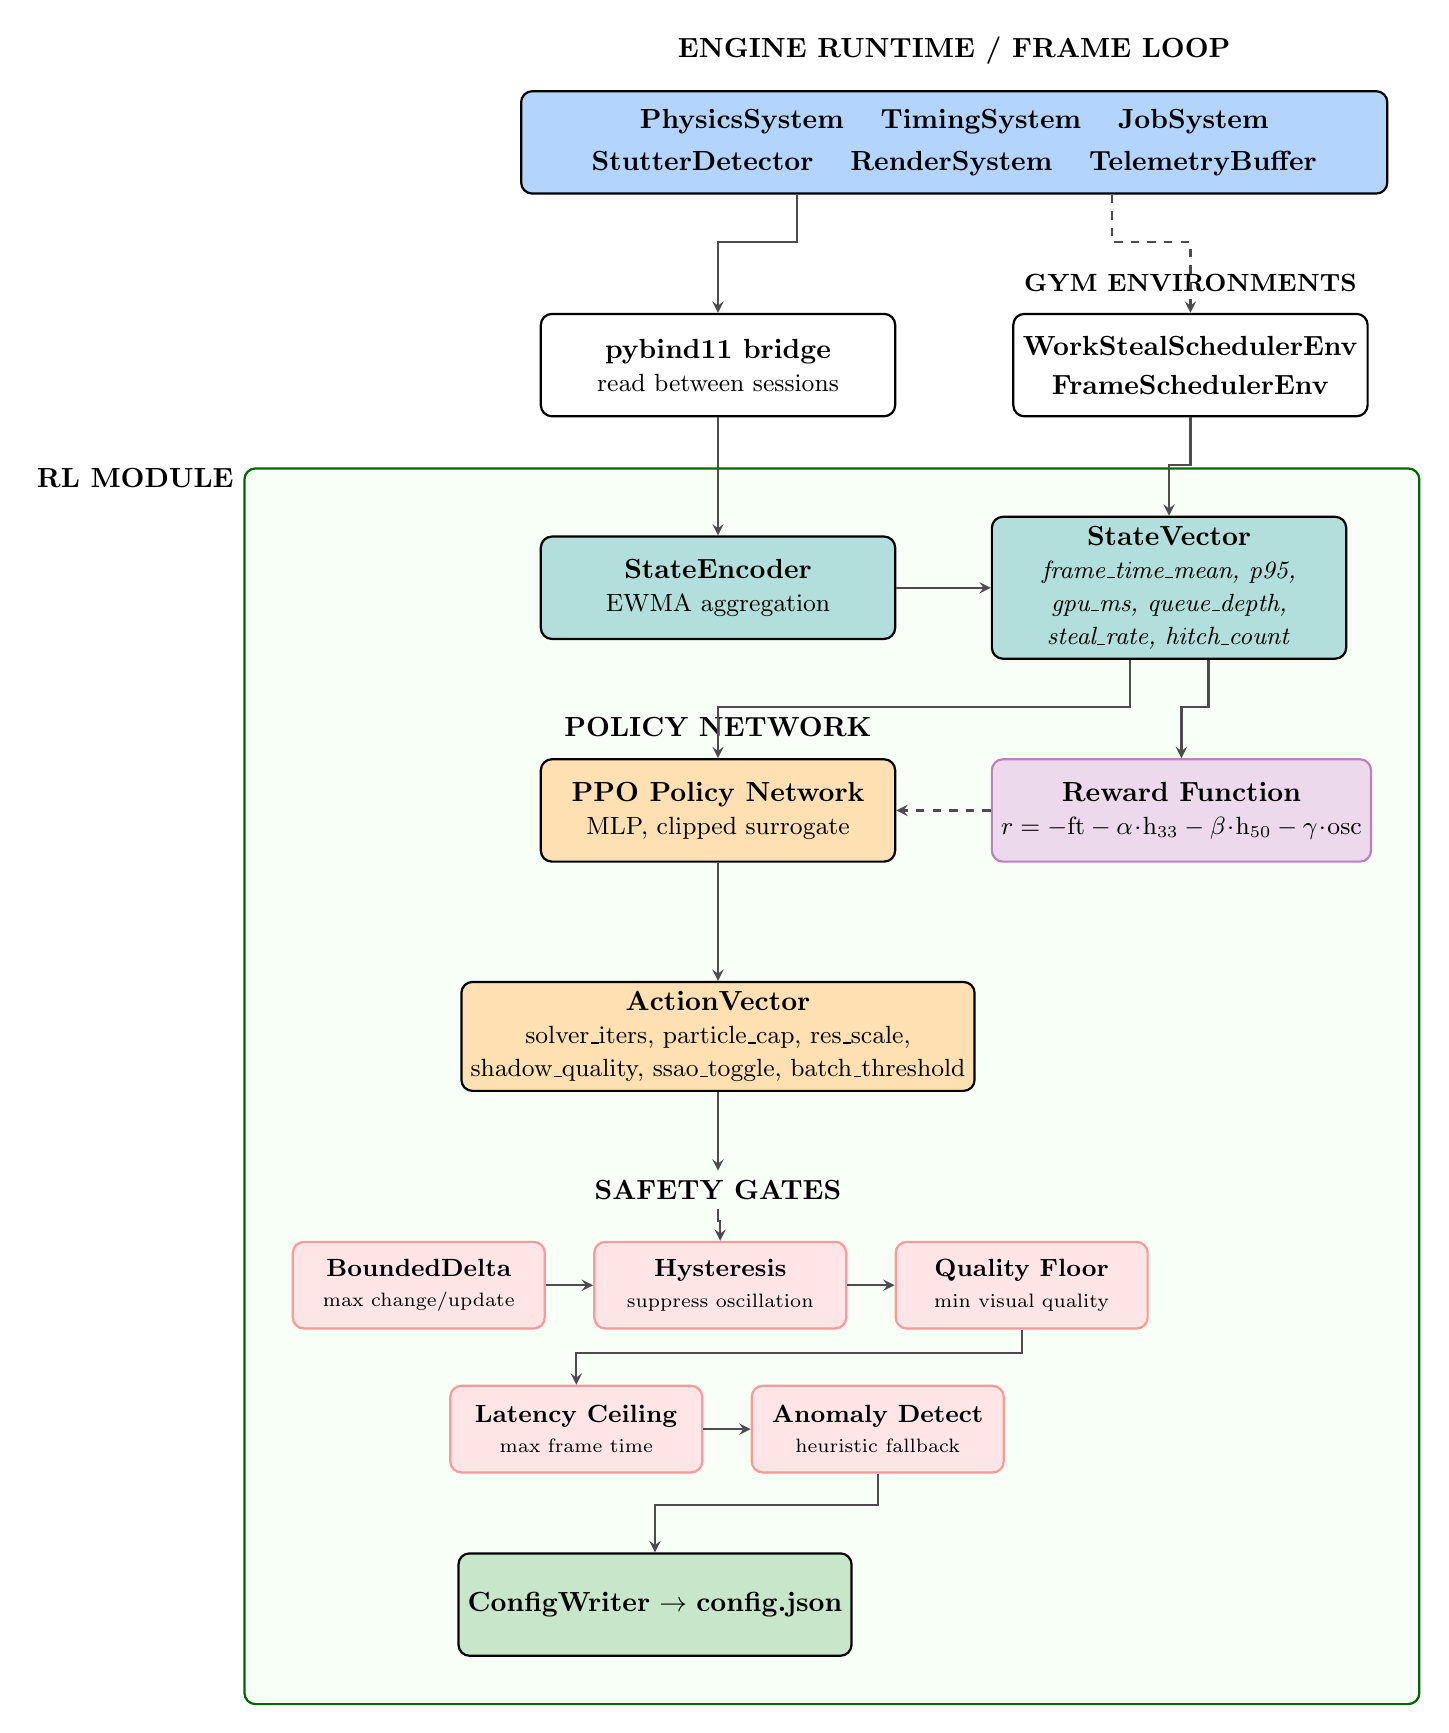
\begin{tikzpicture}[node distance=1.2cm and 1.0cm,
  every node/.style={text=black, font=\normalsize},
  arr/.style={->, >=stealth, thick, draw=black!70},
  bigblock/.style={draw, thick, rounded corners=4pt, minimum width=4.5cm,
                   minimum height=1.3cm, align=center},
  wideblock/.style={draw, thick, rounded corners=4pt, minimum width=11cm,
                    minimum height=1.3cm, align=center},
  gateblock/.style={draw=red!40, thick, fill=red!10, rounded corners=4pt,
                    minimum width=3.2cm, minimum height=1.1cm,
                    align=center, font=\small}]

  %% ═══════════════════════════════════════════════════════════════
  %% ROW 1: FRAME LOOP
  %% ═══════════════════════════════════════════════════════════════

  \node[wideblock, fill=blueBoxLight] (frameloop)
      {\textbf{PhysicsSystem} \quad \textbf{TimingSystem} \quad \textbf{JobSystem}\\[3pt]
       \textbf{StutterDetector} \quad \textbf{RenderSystem} \quad \textbf{TelemetryBuffer}};

  \node[font=\normalsize\bfseries, above=0.2cm of frameloop] {ENGINE RUNTIME / FRAME LOOP};

  %% ═══════════════════════════════════════════════════════════════
  %% ROW 2: PYBIND11 + GYM ENVS
  %% ═══════════════════════════════════════════════════════════════

  \node[bigblock, fill=white, draw=black, below=1.5cm of frameloop, xshift=-3.0cm]
      (pyb) {\textbf{pybind11 bridge}\\{\small read between sessions}};

  \node[bigblock, fill=white, draw=black, below=1.5cm of frameloop, xshift=3.0cm]
      (gym) {\textbf{WorkStealSchedulerEnv}\\[2pt]\textbf{FrameSchedulerEnv}};
  \node[font=\small\bfseries, above=0.15cm of gym] {GYM ENVIRONMENTS};

  \draw[arr] ([xshift=-2.0cm]frameloop.south) -- ++(0,-0.6) -| (pyb.north);
  \draw[arr, dashed] ([xshift=2.0cm]frameloop.south) -- ++(0,-0.6) -| (gym.north);

  %% ═══════════════════════════════════════════════════════════════
  %% ROW 3: STATE ENCODER → STATE VECTOR
  %% ═══════════════════════════════════════════════════════════════

  \node[bigblock, fill=tealBoxLight, below=1.5cm of pyb]
      (senc) {\textbf{StateEncoder}\\{\small EWMA aggregation}};
  \node[bigblock, fill=tealBoxLight, right=1.2cm of senc]
      (svec) {\textbf{StateVector}\\{\small\textit{frame\_time\_mean, p95,}}\\{\small\textit{gpu\_ms, queue\_depth,}}\\{\small\textit{steal\_rate, hitch\_count}}};

  \draw[arr] (pyb.south) -- ++(0,-0.6) -| (senc.north);
  \draw[arr] (gym.south) -- ++(0,-0.6) -| (svec.north);
  \draw[arr] (senc) -- (svec);

  %% ═══════════════════════════════════════════════════════════════
  %% ROW 4: PPO POLICY + REWARD
  %% ═══════════════════════════════════════════════════════════════

  \node[bigblock, fill=orangeBoxLight, below=1.5cm of senc]
      (ppo) {\textbf{PPO Policy Network}\\{\small MLP, clipped surrogate}};
  \node[font=\normalsize\bfseries, above=0.15cm of ppo] {POLICY NETWORK};

  \node[bigblock, fill=violet!15, draw=violet!50, thick, right=1.2cm of ppo]
      (rew) {\textbf{Reward Function}\\{\small$r = -\text{ft} -\alpha\!\cdot\!\text{h}_{33} -\beta\!\cdot\!\text{h}_{50} -\gamma\!\cdot\!\text{osc}$}};

  \draw[arr] ([xshift=-0.5cm]svec.south) -- ++(0,-0.6) -| (ppo.north);
  \draw[arr] ([xshift=0.5cm]svec.south) -- ++(0,-0.6) -| (rew.north);
  \draw[arr, dashed] (rew.west) -- (ppo.east);

  %% ═══════════════════════════════════════════════════════════════
  %% ROW 5: ACTION VECTOR
  %% ═══════════════════════════════════════════════════════════════

  \node[bigblock, fill=orangeBoxLight, below=1.5cm of ppo]
      (avec) {\textbf{ActionVector}\\{\small solver\_iters, particle\_cap, res\_scale,}\\{\small shadow\_quality, ssao\_toggle, batch\_threshold}};

  \draw[arr] (ppo) -- (avec);

  %% ═══════════════════════════════════════════════════════════════
  %% ROW 6: SAFETY GATES (3 + 2 grid)
  %% ═══════════════════════════════════════════════════════════════

  \node[font=\normalsize\bfseries, below=1.0cm of avec] (sglbl) {SAFETY GATES};

  \node[gateblock, below=0.4cm of sglbl, xshift=-3.8cm]
      (bd)   {\textbf{BoundedDelta}\\{\scriptsize max change/update}};
  \node[gateblock, right=0.6cm of bd]
      (hyst) {\textbf{Hysteresis}\\{\scriptsize suppress oscillation}};
  \node[gateblock, right=0.6cm of hyst]
      (qf)   {\textbf{Quality Floor}\\{\scriptsize min visual quality}};

  \node[gateblock, below=0.7cm of bd, xshift=2.0cm]
      (lc)   {\textbf{Latency Ceiling}\\{\scriptsize max frame time}};
  \node[gateblock, right=0.6cm of lc]
      (anom) {\textbf{Anomaly Detect}\\{\scriptsize heuristic fallback}};

  \draw[arr] (avec.south) -- (sglbl.north);
  \draw[arr] (sglbl.south) -- ++(0,-0.15) -| (hyst.north);

  \draw[arr] (bd)   -- (hyst);
  \draw[arr] (hyst) -- (qf);
  \draw[arr] (qf.south) -- ++(0,-0.3) -| (lc.north);
  \draw[arr] (lc)   -- (anom);

  %% ═══════════════════════════════════════════════════════════════
  %% ROW 7: CONFIG OUTPUT
  %% ═══════════════════════════════════════════════════════════════

  \node[bigblock, fill=greenBoxLight, thick, below=1.0cm of lc, xshift=1.0cm]
      (cw) {\textbf{ConfigWriter} $\rightarrow$ \textbf{config.json}};

  \draw[arr] (anom.south) -- ++(0,-0.4) -| (cw.north);

  %% ═══════════════════════════════════════════════════════════════
  %% RL MODULE outer group
  %% ═══════════════════════════════════════════════════════════════

  \begin{scope}[on background layer]
    \node[draw=green!40!black, thick, fill=green!3, rounded corners,
          inner sep=0.6cm,
          fit=(senc)(svec)(ppo)(rew)(avec)(bd)(hyst)(qf)(lc)(anom)(cw)(sglbl),
          label={[font=\normalsize\bfseries, text=black]above left:RL MODULE}] (rlmod) {};
  \end{scope}

\end{tikzpicture}
\caption{RL auto-tuner architecture: per-frame telemetry flows through pybind11 into
         gym environments, is encoded via EWMA, evaluated by PPO, validated through
         safety gates, and written to config for the next session.}
\label{fig:rl_full_pipeline}
\end{figure}

\section{Telemetry and State Encoding}

Telemetry collection runs inside the engine's frame loop across six subsystems shown in the top row of Figure~\ref{fig:rl_full_pipeline}. PhysicsSystem reports solver iteration counts and active particle counts. TimingSystem measures CPU frame duration and GPU time using \texttt{GL\_ARB\_timer\_query}. JobSystem records queue depth and steal statistics from the work-stealing deques. StutterDetector flags any frame that exceeds 33.3\,ms (a 30\,fps miss) or 50\,ms (a 20\,fps miss). RenderSystem logs draw call counts and GPU submission timing. TelemetryBuffer stores all of these signals in a ring buffer that survives across frames and is persisted to disk at session end.

Between sessions, the pybind11 bridge reads this persisted buffer and hands it to the StateEncoder. The StateEncoder applies exponentially weighted moving averages to smooth out per-frame noise and capture recent performance trends rather than instantaneous spikes. The output is a StateVector with six fields: mean frame time, p95 frame time, GPU time estimate, job queue depth, steal rate, and hitch count. This is deliberately compact. A small state vector keeps policy inference fast and avoids overfitting to transient frame-level noise.

\section{Policy Networks and Safety Gates}

The policy network uses Proximal Policy Optimization (PPO) with a clipped surrogate objective~\cite{ppo}. The clipping is important here because it prevents the policy from making large destructive parameter changes in a single update, which matters when those parameters directly affect whether a classroom demo runs smoothly. The network itself is a straightforward MLP. Deep Deterministic Policy Gradient (DDPG) is also supported as an alternative for strictly continuous action spaces~\cite{lillicrap2016ddpg}. Training uses the two Gymnasium environments (FrameSchedulerEnv and WorkStealSchedulerEnv) to simulate workload variability, and metrics are logged through TensorBoard. Reproducibility practices follow guidance from Henderson et al.~\cite{henderson_rl_matters}.

The reward function shown in Figure~\ref{fig:rl_full_pipeline} is:
\[
  r = -\text{ft} - \alpha \cdot h_{33} - \beta \cdot h_{50} - \gamma \cdot \text{osc}
\]
where ft is mean frame time, $h_{33}$ counts frames exceeding the 33\,ms threshold, $h_{50}$ counts frames exceeding 50\,ms, and osc penalises oscillation in configuration values between sessions. The weighting coefficients $\alpha$, $\beta$, $\gamma$ are tuned to prioritise stability over raw throughput. A configuration that holds a steady 30\,fps is preferred over one that averages 60\,fps but hitches regularly.

The policy outputs an action vector with six parameters: solver iteration count, particle cap, resolution scale, shadow quality level, SSAO toggle, and batching threshold. These are the knobs the auto-tuner is allowed to adjust.

Before any of these values reach disk, they pass through five safety gates arranged in sequence (shown in the bottom half of Figure~\ref{fig:rl_full_pipeline}):

\textbf{BoundedDelta} limits how much any single parameter can change per update. Even if the policy wants to cut solver iterations from 20 to 2, BoundedDelta will only allow a step of a few iterations at a time.

\textbf{Hysteresis} suppresses oscillation. If the policy keeps flipping a parameter back and forth between sessions, hysteresis locks the value until a consistent trend emerges.

\textbf{Quality Floor} enforces minimum visual quality. No matter what the policy suggests, certain settings (like minimum shadow resolution or minimum particle count) cannot drop below a defined threshold.

\textbf{Latency Ceiling} enforces a maximum acceptable frame time. If a proposed configuration would push frame time above the ceiling based on recent telemetry, the change is rejected.

\textbf{Anomaly Detect} catches cases where telemetry looks abnormal (for example, a sudden spike caused by a background OS process rather than an actual workload problem). When triggered, it falls back to a deterministic heuristic configuration instead of trusting the policy output.

Only configurations that survive all five gates are written to \texttt{config.json} by the ConfigWriter~\cite{cpo, safe_rl_survey}.


\section{Session Boundary Application Model}

The separation between the RL module and the running engine is strict and intentional. During a live session, the engine reads its configuration once at startup and never modifies it. Telemetry is collected but nothing changes. The simulation behaves identically every time it runs with the same config file, which means a teacher can demonstrate the same scenario repeatedly and get the same results.

After the session ends, the RL module wakes up, reads aggregated telemetry, runs policy inference, validates the output through the safety gates, and writes an updated config file if it finds an improvement. On the next startup, the engine loads this new configuration.

This design means the auto-tuner progressively adapts to whatever hardware the engine is running on, session by session, without ever surprising the user during a live demonstration. A teacher running the engine on a ten-year-old classroom laptop will see the system gradually converge toward settings that hold a stable frame rate on that machine. A teacher on a newer workstation will converge toward higher quality settings. In both cases, the behaviour during any given session is fully deterministic and predictable.

\chapter{Results}
\label{chap:results}

This chapter presents empirical results across four evaluation domains:
prototype evolution, the visual authoring editor, simulation subsystems, and
the passive reinforcement learning auto-tuner.  All benchmarks were conducted
on a machine running Ubuntu 22.04 with an NVIDIA GeForce GTX 1650 and
11 logical CPU cores.  Frame time is reported in milliseconds; lower values
are better.  Standard deviation and p95 latency are included where relevant
to characterise stability rather than peak performance alone.

% ═══════════════════════════════════════════════════════════════════════════
\section{Prototype Demonstrations}
% ═══════════════════════════════════════════════════════════════════════════

\subsection{Phase 1: Verlet Cloth Prototypes}

The first prototypes implemented mass-spring cloth using Verlet integration.
Figure~\ref{fig:verlet1} shows the undisturbed cloth mesh under gravity,
demonstrating stable draping.  Figures~\ref{fig:verlet2} and~\ref{fig:verlet3}
show progressive constraint deletion after successive cannon impacts,
exposing the tearing behaviour that motivated the transition to XPBD.  At
59~FPS the simulator ran comfortably in real time, but stiffness calibration
was timestep-dependent and high spring constants produced visible divergence,
directly motivating the adoption of Extended Position-Based Dynamics.

\begin{figure}[H]
  \centering
  \begin{subfigure}[t]{0.32\textwidth}
    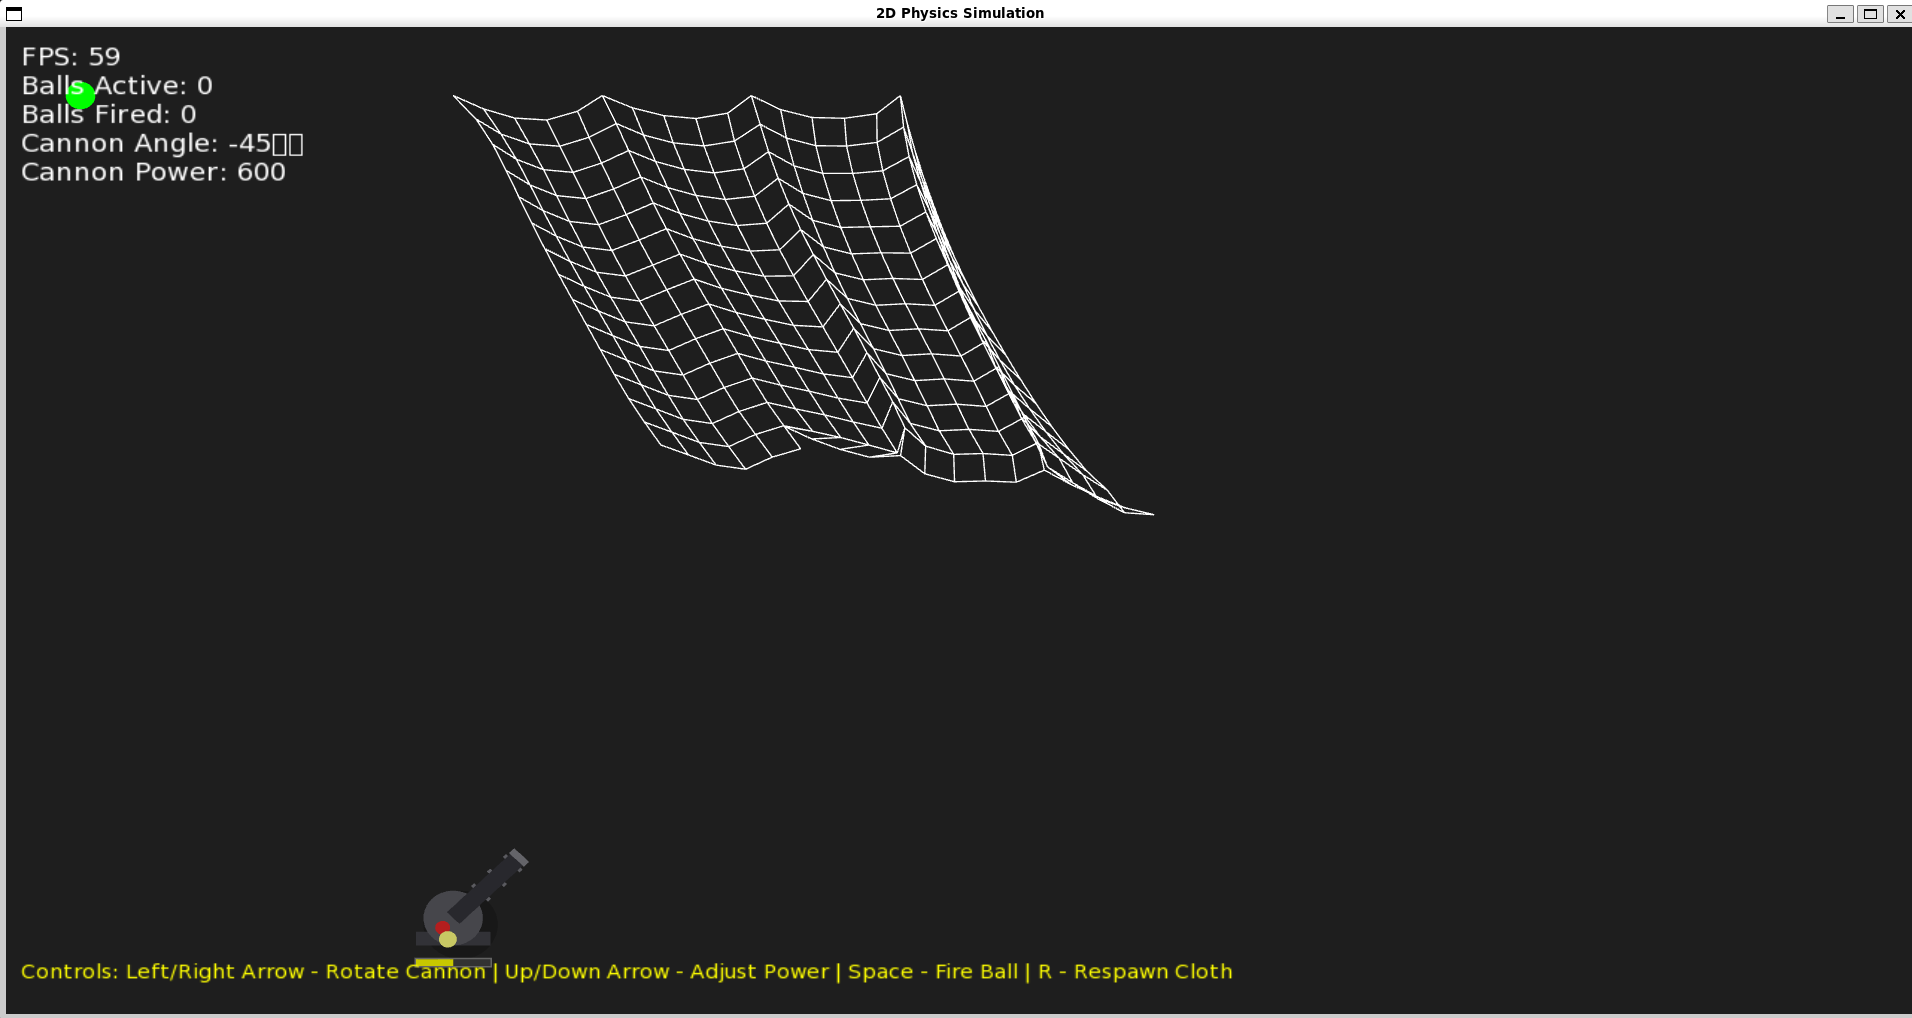
\includegraphics[width=\textwidth]{images/VertletDemo.png}
    \caption{Undisturbed cloth.}
    \label{fig:verlet1}
  \end{subfigure}\hfill
  \begin{subfigure}[t]{0.32\textwidth}
    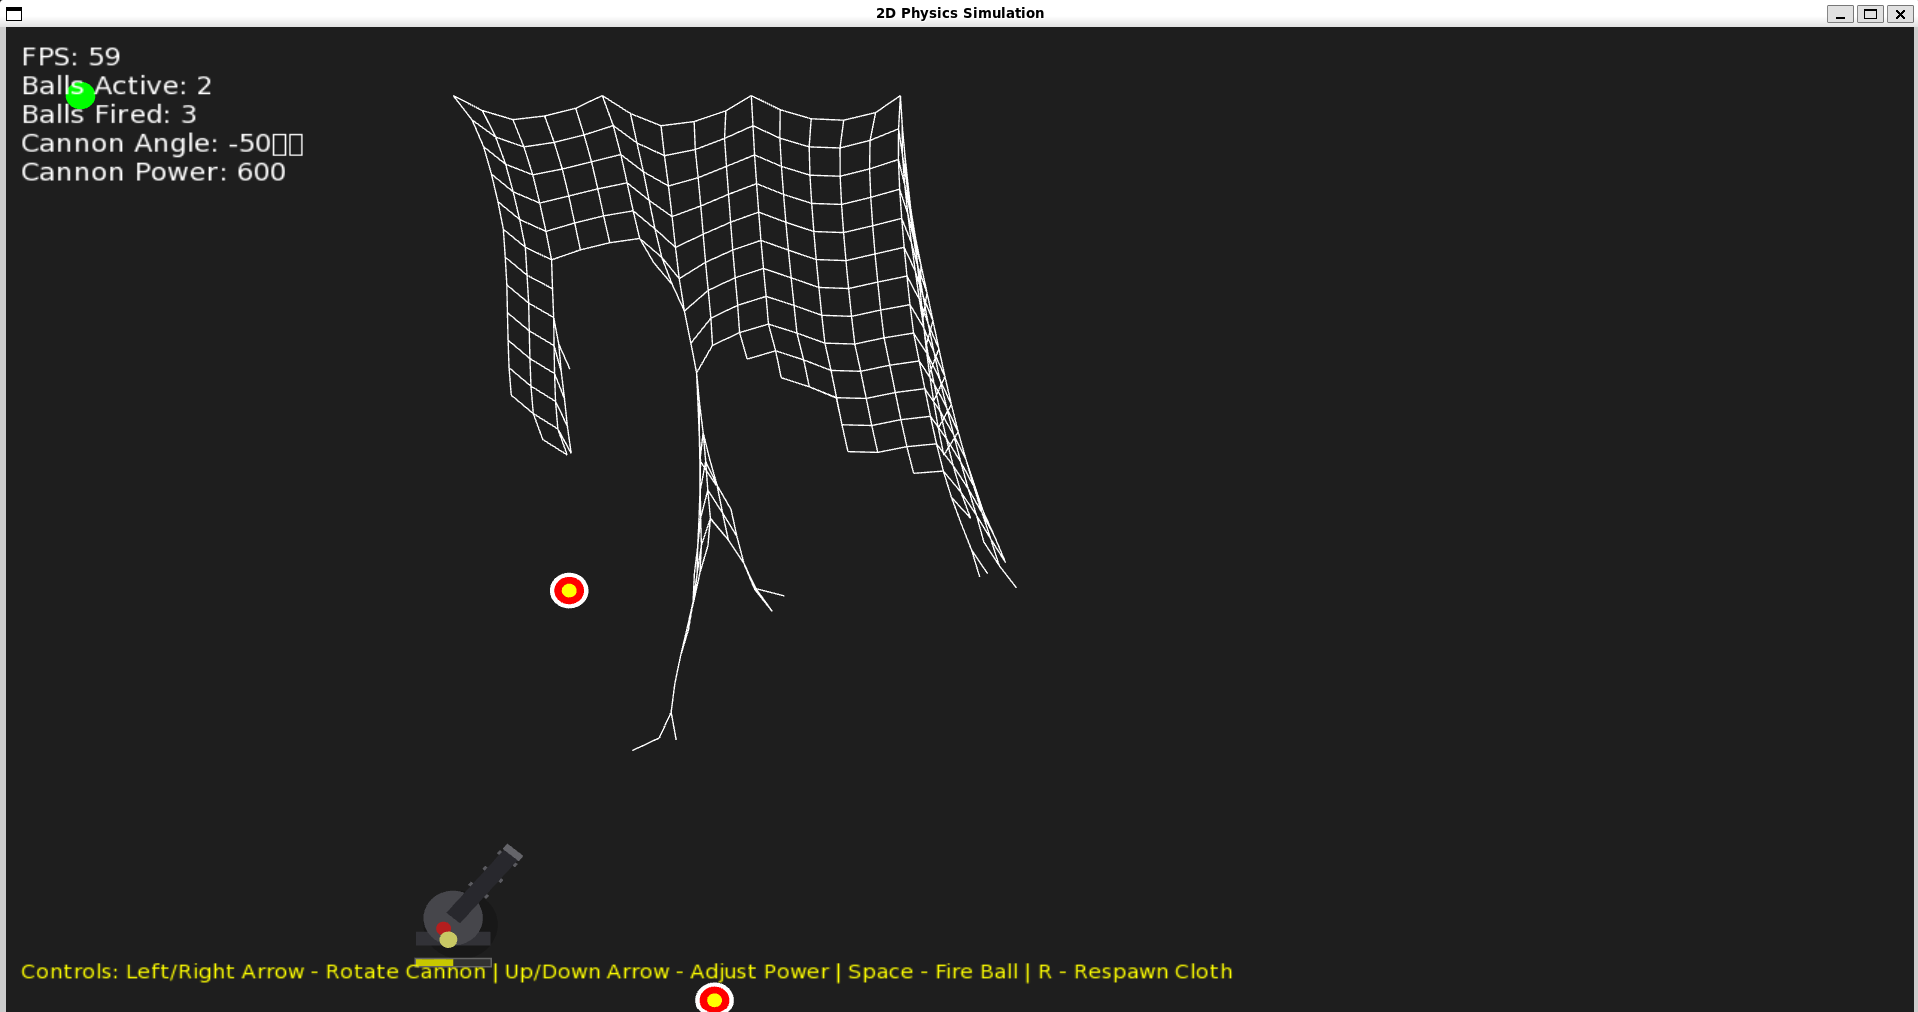
\includegraphics[width=\textwidth]{images/VertletDemo2.png}
    \caption{First impact tear.}
    \label{fig:verlet2}
  \end{subfigure}\hfill
  \begin{subfigure}[t]{0.32\textwidth}
    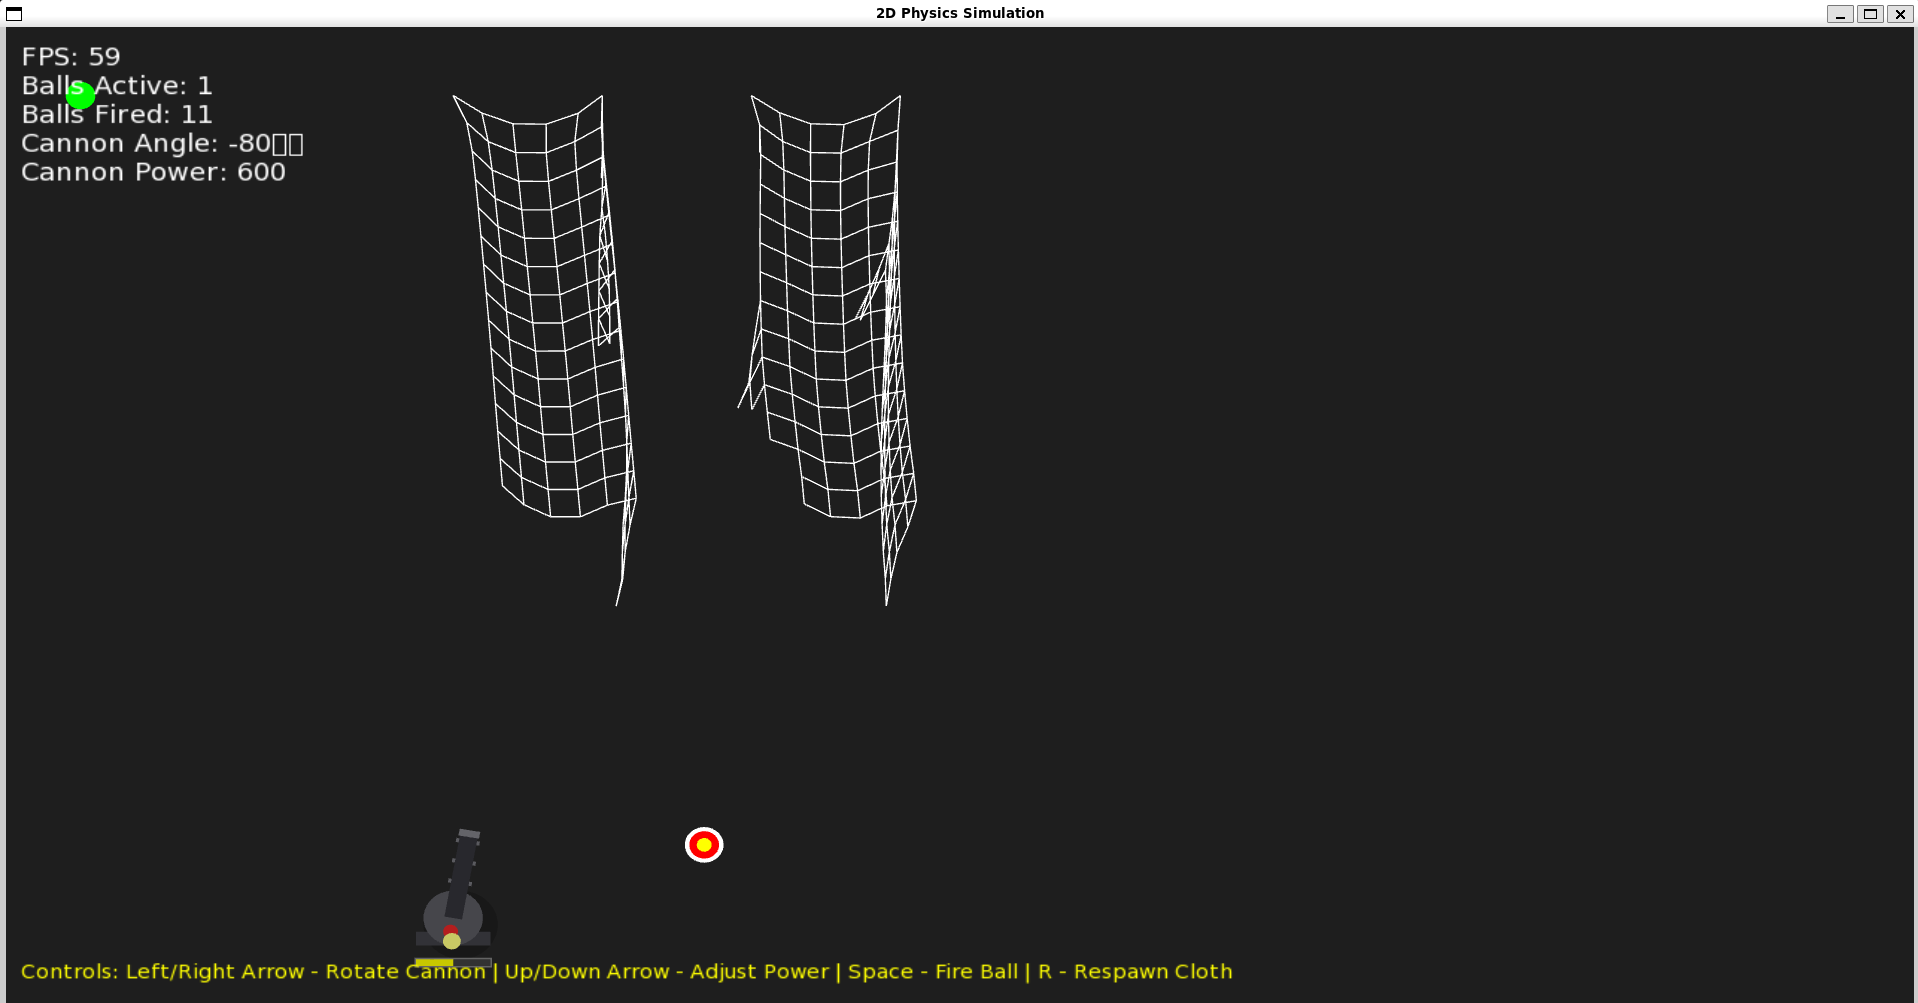
\includegraphics[width=\textwidth]{images/VertletDemo3.png}
    \caption{Multiple tears after repeated impacts.}
    \label{fig:verlet3}
  \end{subfigure}
  \caption{Phase 1 Verlet cloth prototype showing tearing under cannon impact.}
  \label{fig:verlet_proto}
\end{figure}

\subsection{Phase 2: Robosim Robotics Prototype}

The robotics prototype implemented a six-joint serial arm using
Denavit--Hartenberg parameters and Jacobian-transpose inverse kinematics.
Figures~\ref{fig:joint1} and~\ref{fig:joint2} show the arm at two
configurations with the TCP position, joint PID gains, and DH parameter
table visible.  The prototype confirmed that Jacobian-transpose methods are
sufficient for interactive demonstrations and that procedural geometry removes
the need for an external asset pipeline.  The performance overlay reported
152~ms per frame (6.6~FPS), which reflected the absence of any parallelism
in the prototype and directly informed the job system design of the final
engine.

\begin{figure}[H]
  \centering
  \begin{subfigure}[t]{0.48\textwidth}
    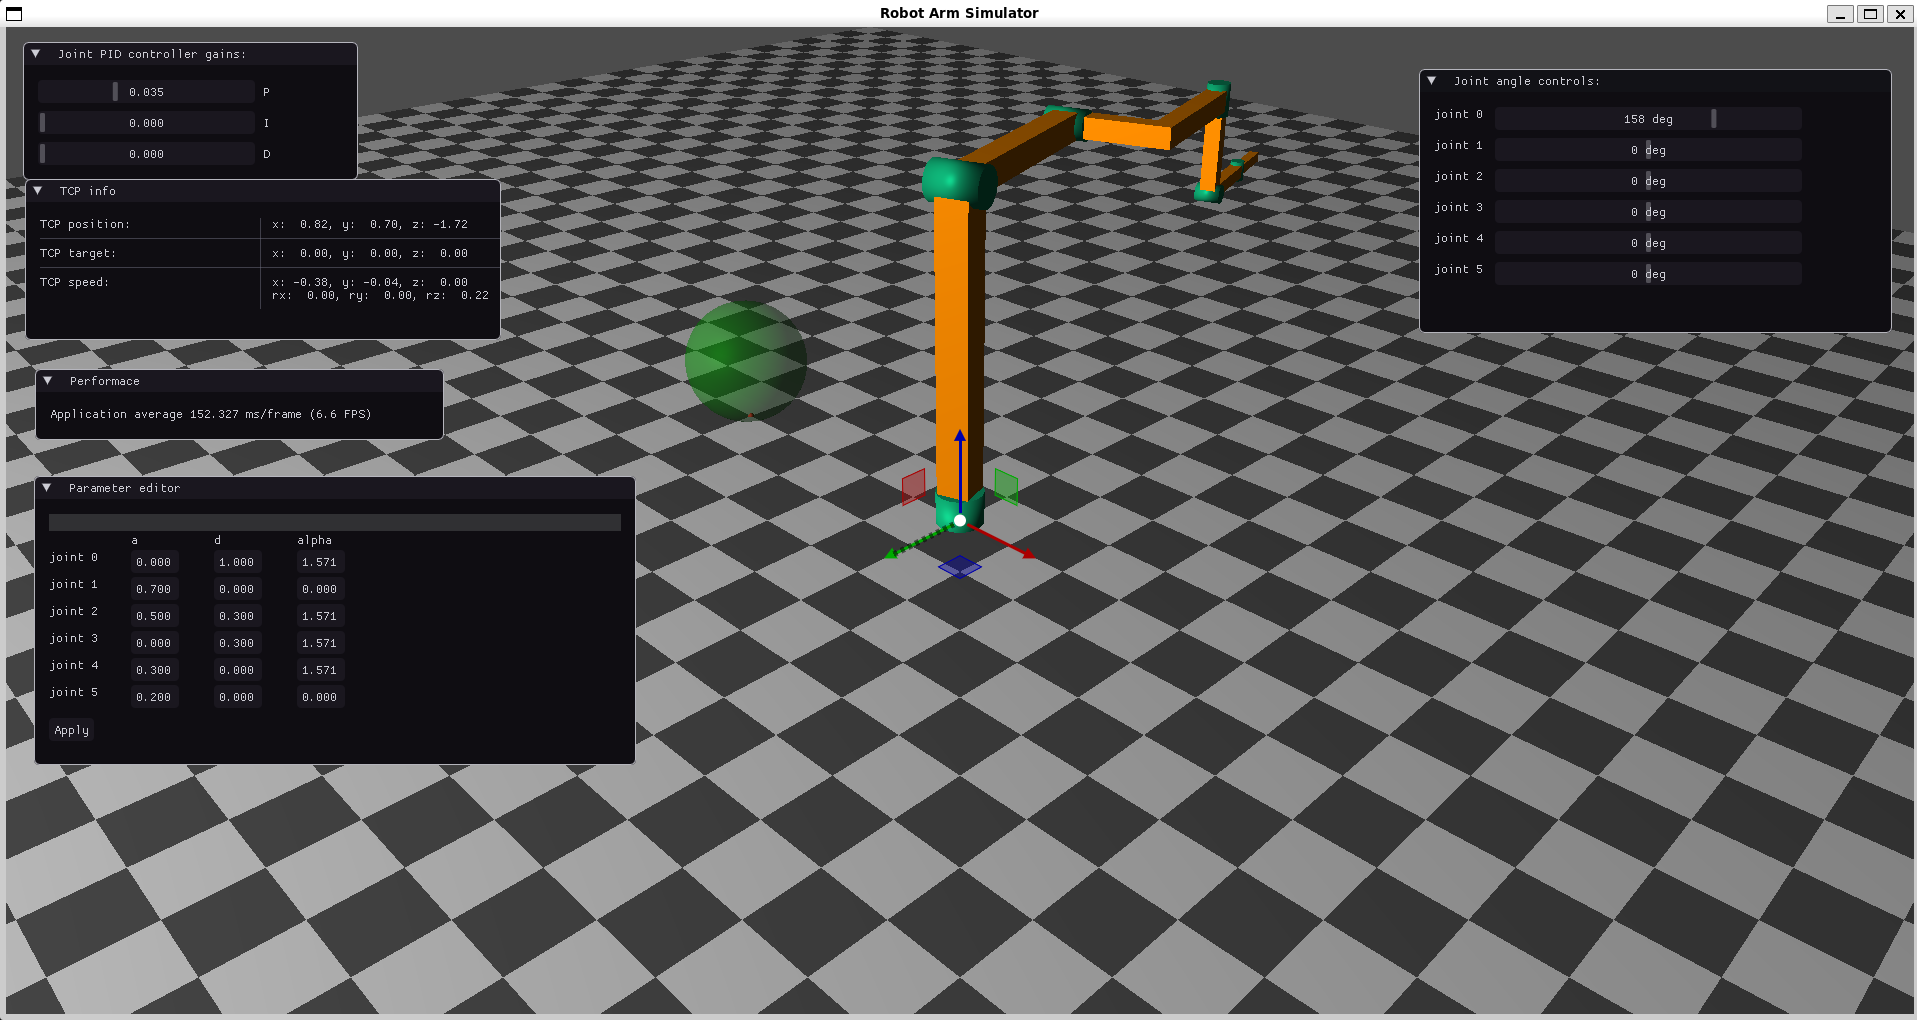
\includegraphics[width=\textwidth]{images/Joint.png}
    \caption{Arm at extended configuration.}
    \label{fig:joint1}
  \end{subfigure}\hfill
  \begin{subfigure}[t]{0.48\textwidth}
    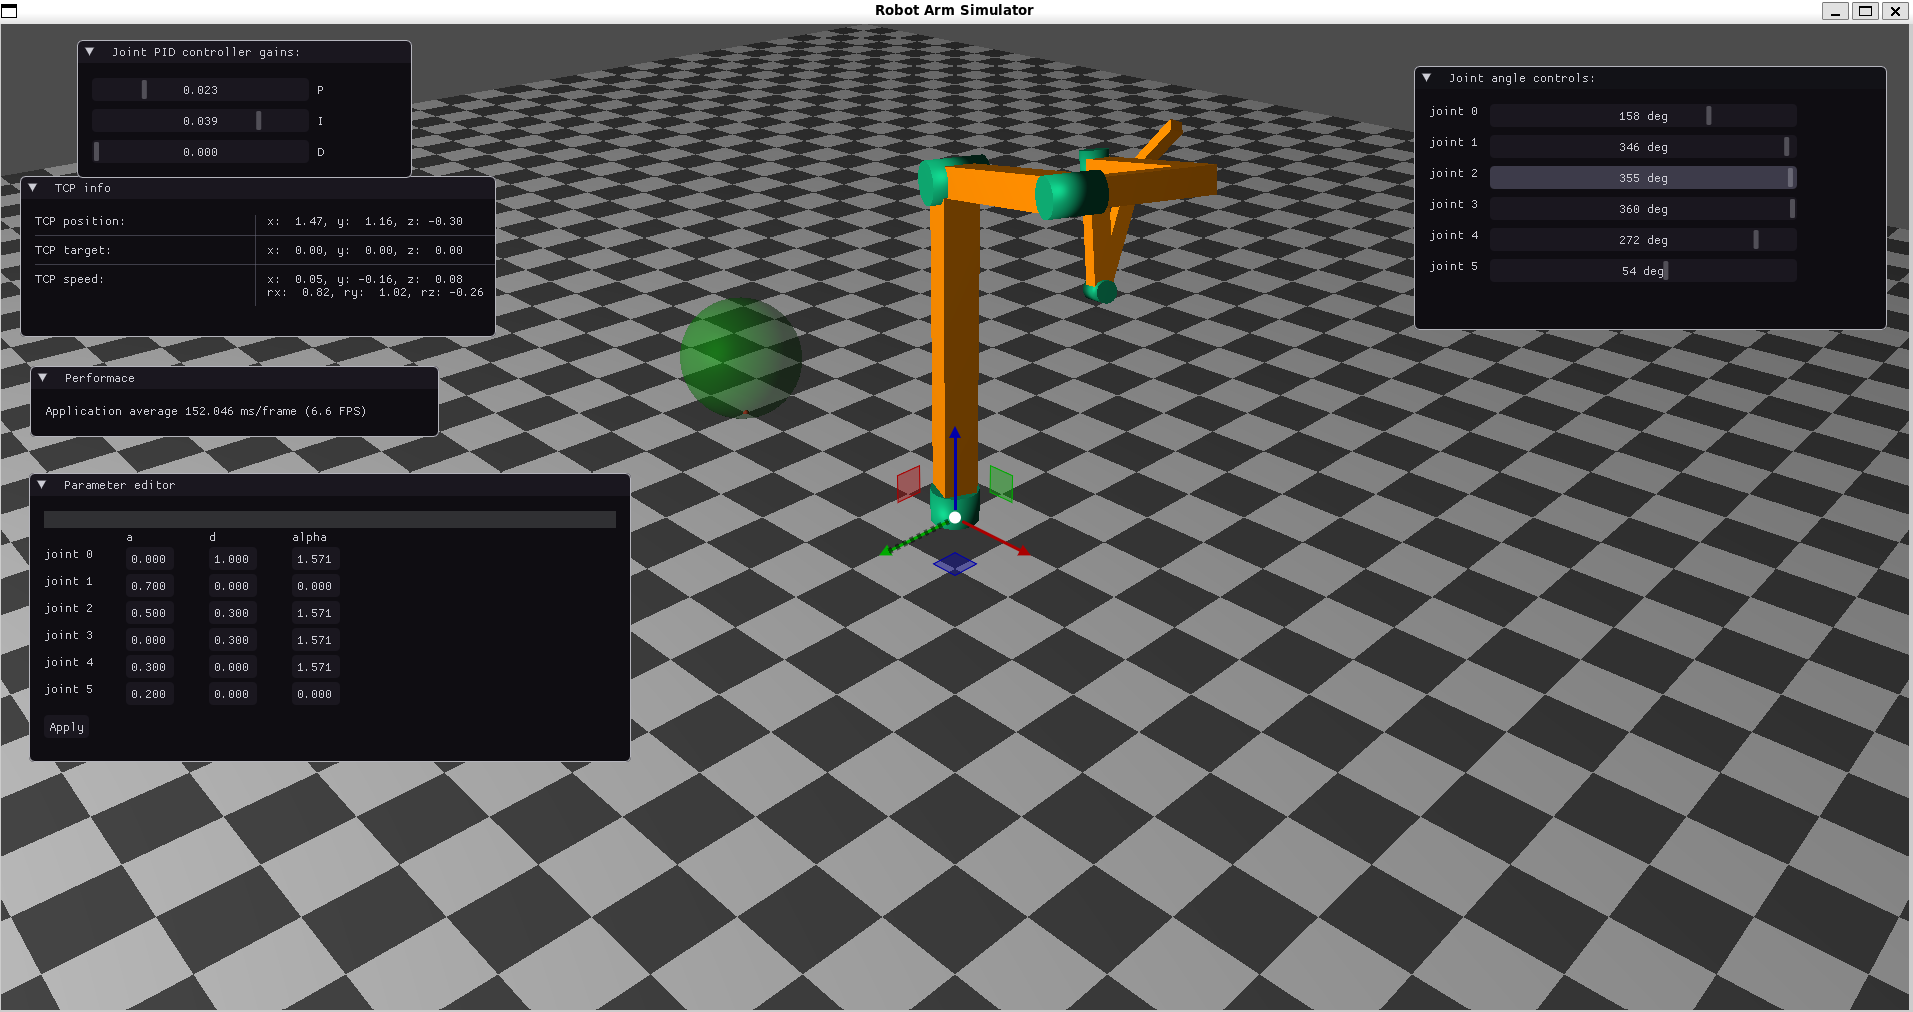
\includegraphics[width=\textwidth]{images/Joint2.png}
    \caption{Arm near home position.}
    \label{fig:joint2}
  \end{subfigure}
  \caption{Phase 2 Robosim prototype showing DH-parameterised six-joint arm
           with live TCP telemetry and PID gain controls.}
  \label{fig:robosim}
\end{figure}



\subsection{Phase 3: Matrix Transform Visualizer}

An interactive 2D matrix transform visualizer was built as a standalone
demonstration for linear algebra concepts.
Figure~\ref{fig:matrix_viz} shows the tool displaying an arrow shape under a
rotation of $-89.2$ degrees. The right panel exposes rotation, scale (X/Y),
and shear (X/Y) as interactive sliders. The resulting $3 \times 3$
transformation matrix is displayed numerically alongside the determinant and
an area preservation indicator. With the current rotation, the determinant
reads 1.000 and the display confirms that area is preserved, which is the
expected result for a pure rotation.

The tool supports four shape primitives (Square, Arrow, House, and Letter F)
that can be cycled with the Tab key, and includes auto-rotate and reset
controls. The original shape is rendered as a ghost outline while the
transformed shape is drawn in solid colour, with x-grid and y-grid lines
showing how the coordinate system itself deforms under the transformation.

This prototype validates the pedagogical scaffolding approach: instead of
asking students to compute matrix entries by hand, the visualizer lets them
drag a slider and immediately see how rotation, scale, and shear map to
specific matrix values and geometric outcomes. The determinant readout
connects the abstract concept of area scaling to a visible quantity that
updates in real time.

\begin{figure}[H]
  \centering
  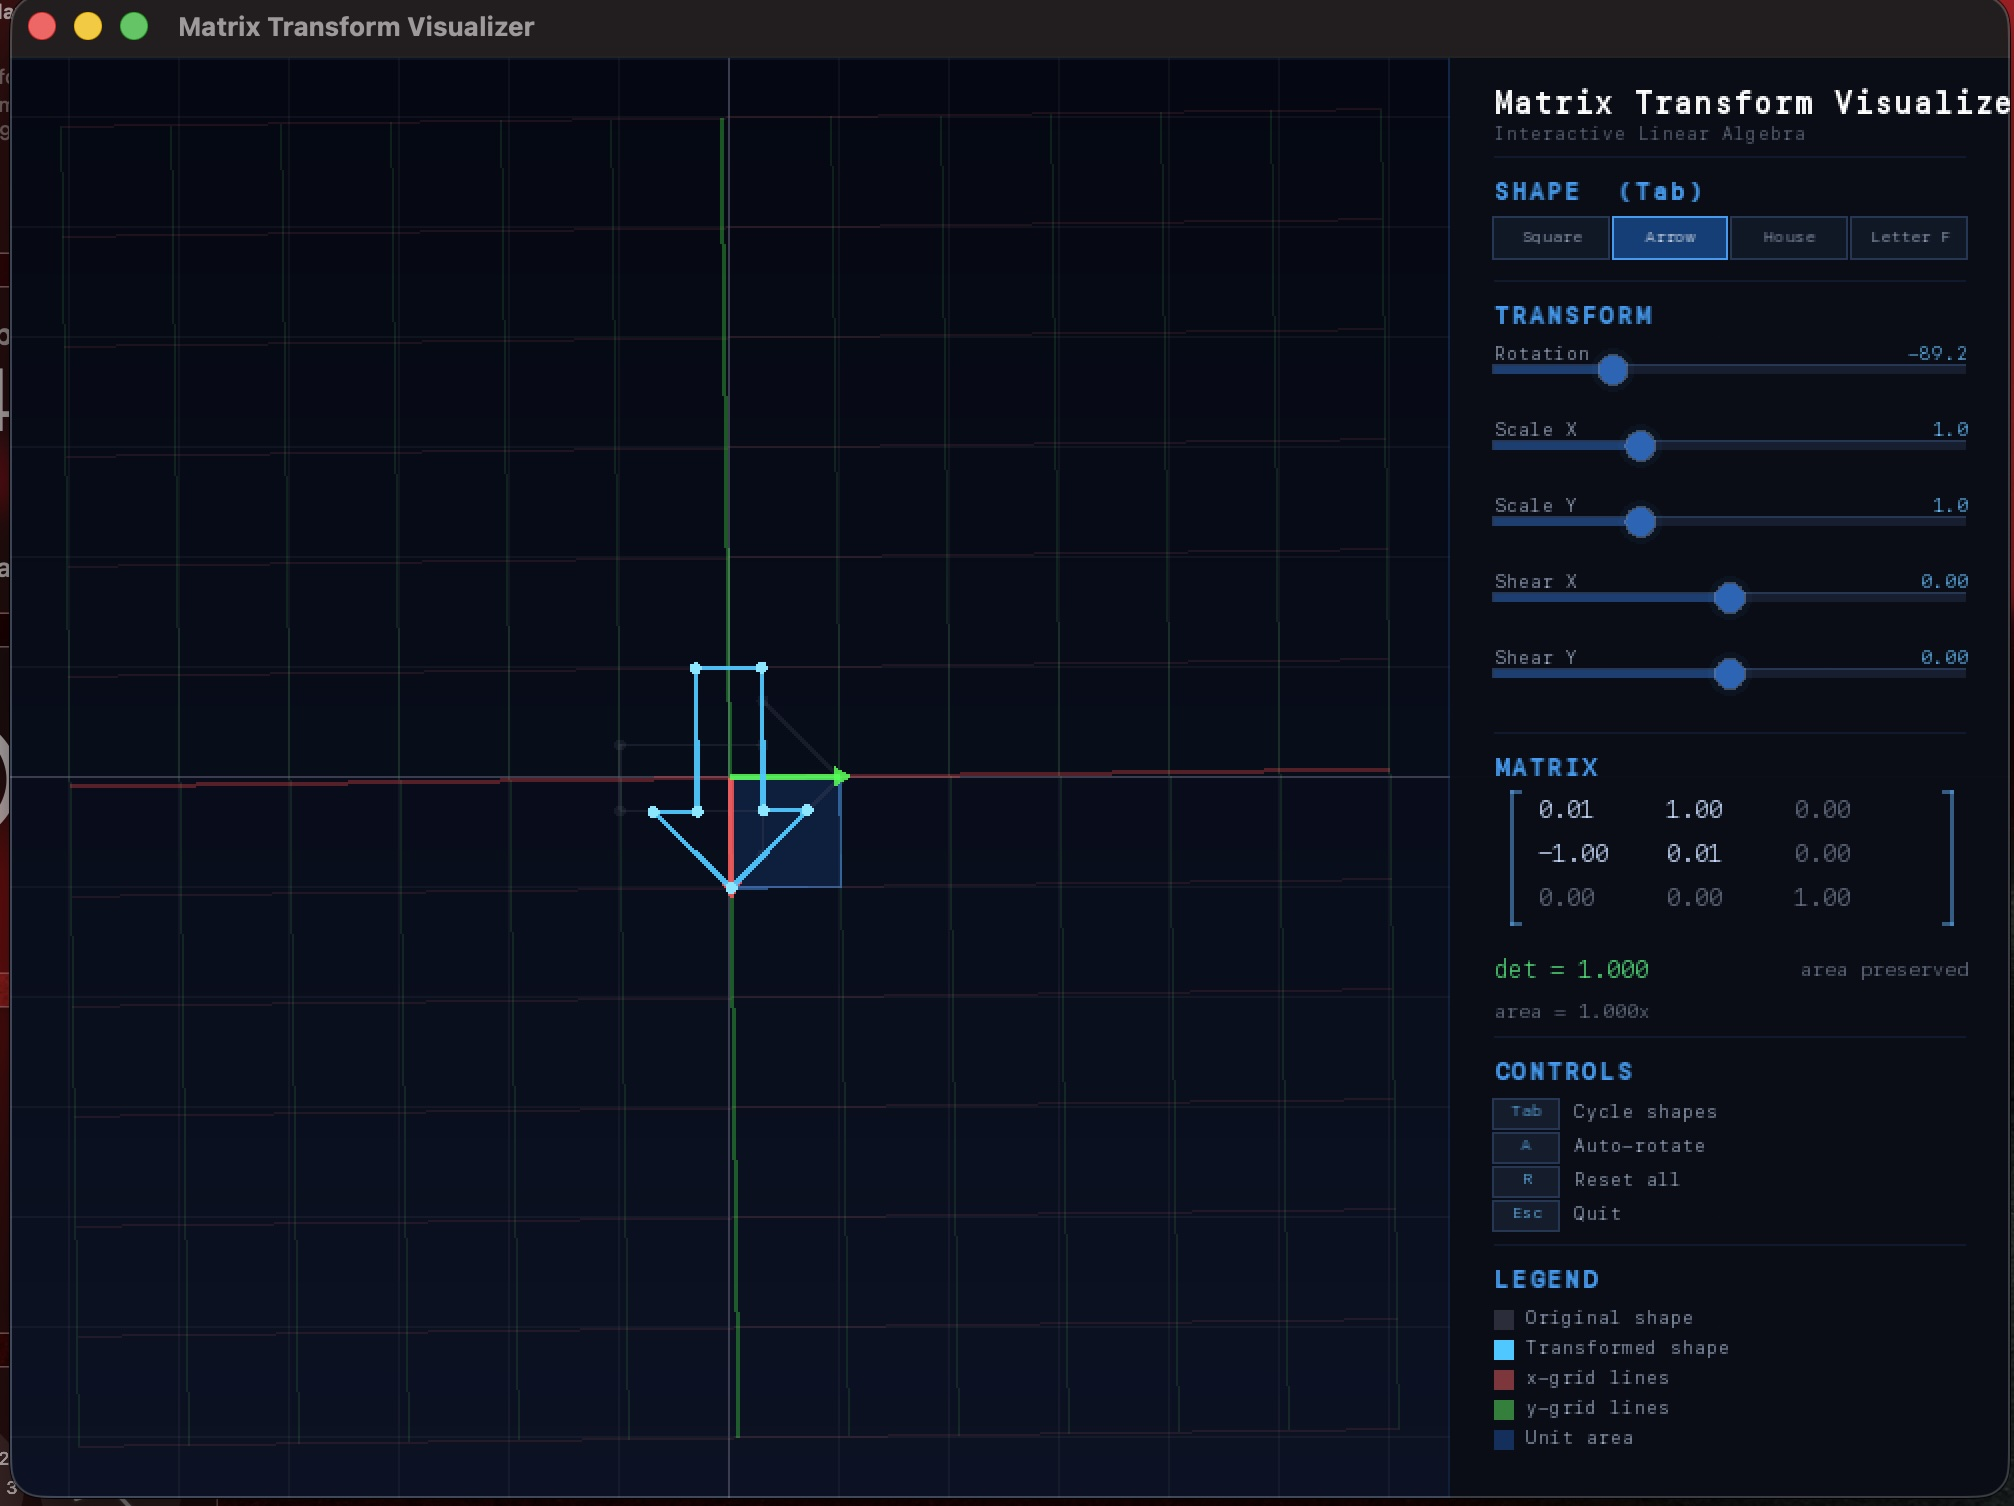
\includegraphics[width=0.85\textwidth]{images/Matrix viz .jpg}
  \caption{Interactive matrix transform visualizer showing an arrow shape
           under $-89.2^\circ$ rotation with live matrix display, determinant
           readout, and area preservation indicator.}
  \label{fig:matrix_viz}
\end{figure}
% ═══════════════════════════════════════════════════════════════════════════
\section{Simulation Subsystem Results}
% ═══════════════════════════════════════════════════════════════════════════

\subsection{XPBD Cloth and Soft Body}

The XPBD cloth simulation was evaluated with 4{,}541 particles and
4 solver iterations.  Figures~\ref{fig:hpbd1}--\ref{fig:hpbd3} show three
representative scenes: a cloth draped over a sphere, rigid body meshes
resting on a cloth platform, and multi-body interaction with the Stanford
Bunny and Armadillo models.  Frame rates ranged from 24 to 42~FPS depending
on the number of active collision constraints.  The compliance parameters
(\texttt{stretch} = 0.0001, \texttt{bend} = 0.0001) remained stable across
all scenes without requiring timestep adjustment, validating the
timestep-invariant property of the XPBD formulation.  The cloth-sphere
interaction in Figure~\ref{fig:hpbd1} produced 57 active collision
constraints simultaneously without instability.

\begin{figure}[H]
  \centering
  \begin{subfigure}[t]{0.32\textwidth}
    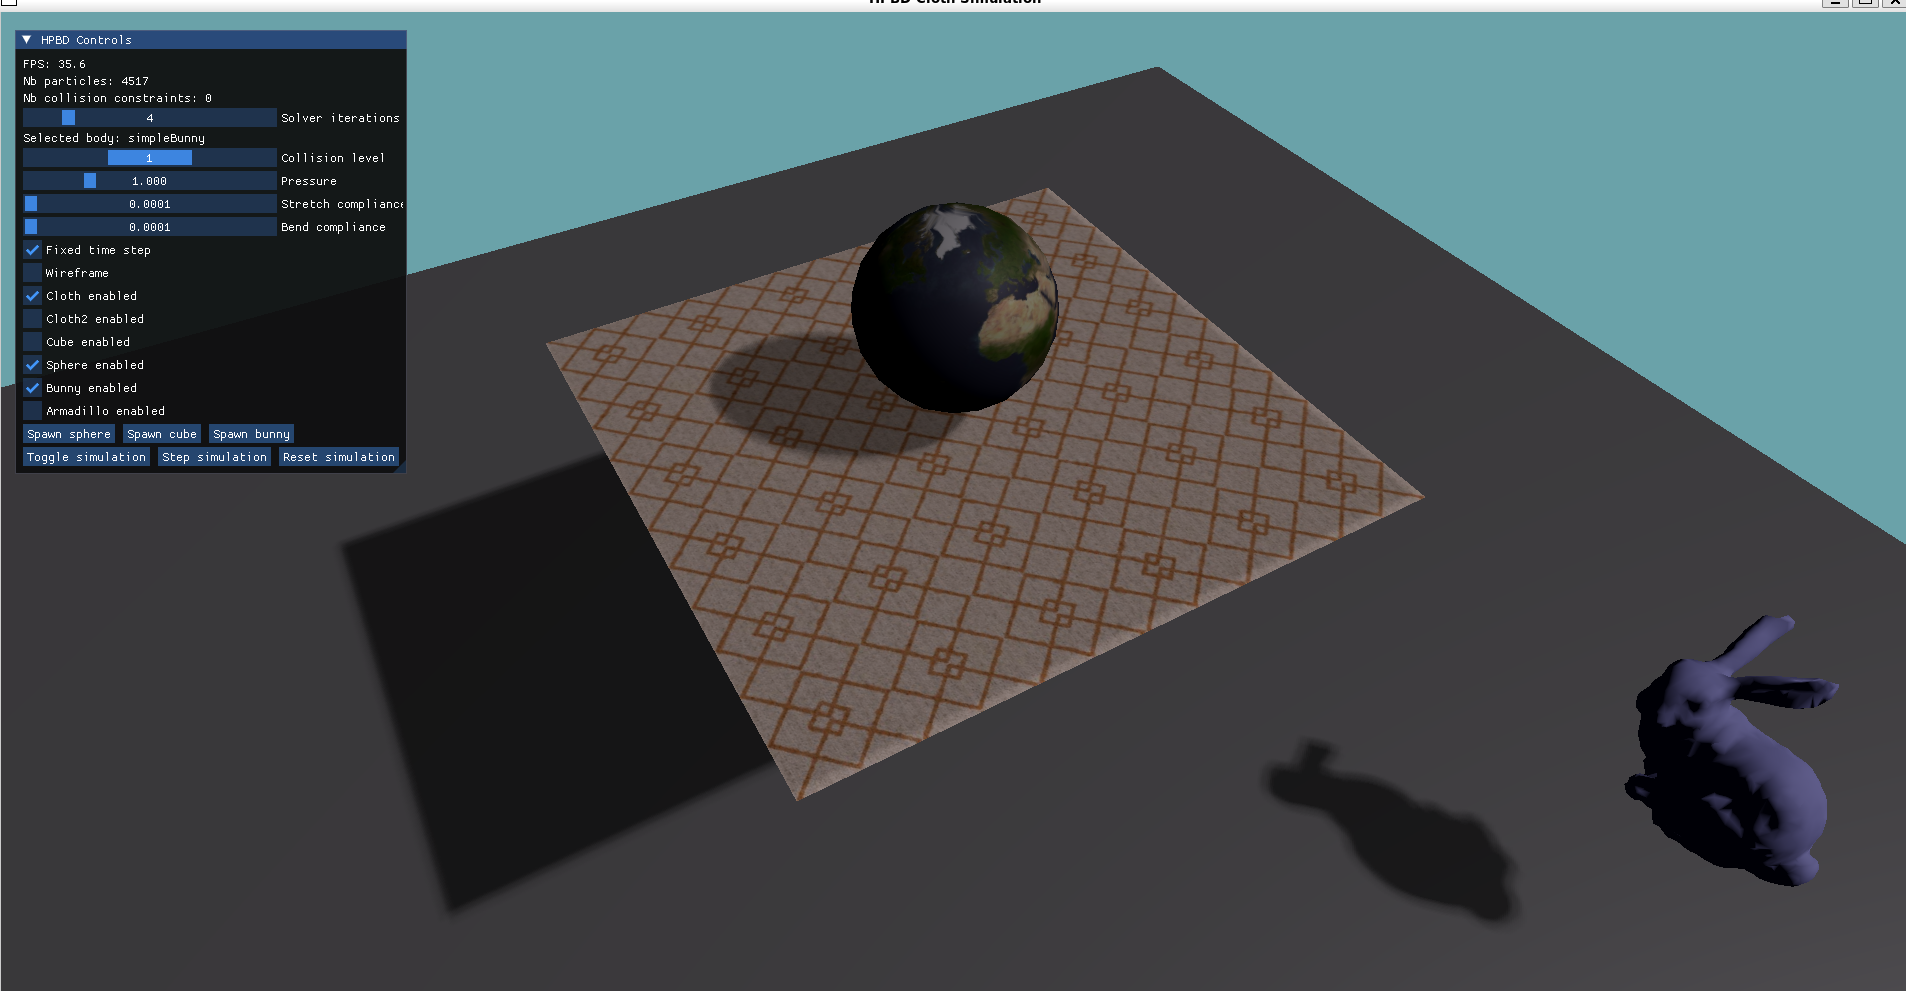
\includegraphics[width=\textwidth]{images/HPBD.png}
    \caption{Cloth draped over sphere.}
    \label{fig:hpbd1}
  \end{subfigure}\hfill
  \begin{subfigure}[t]{0.32\textwidth}
    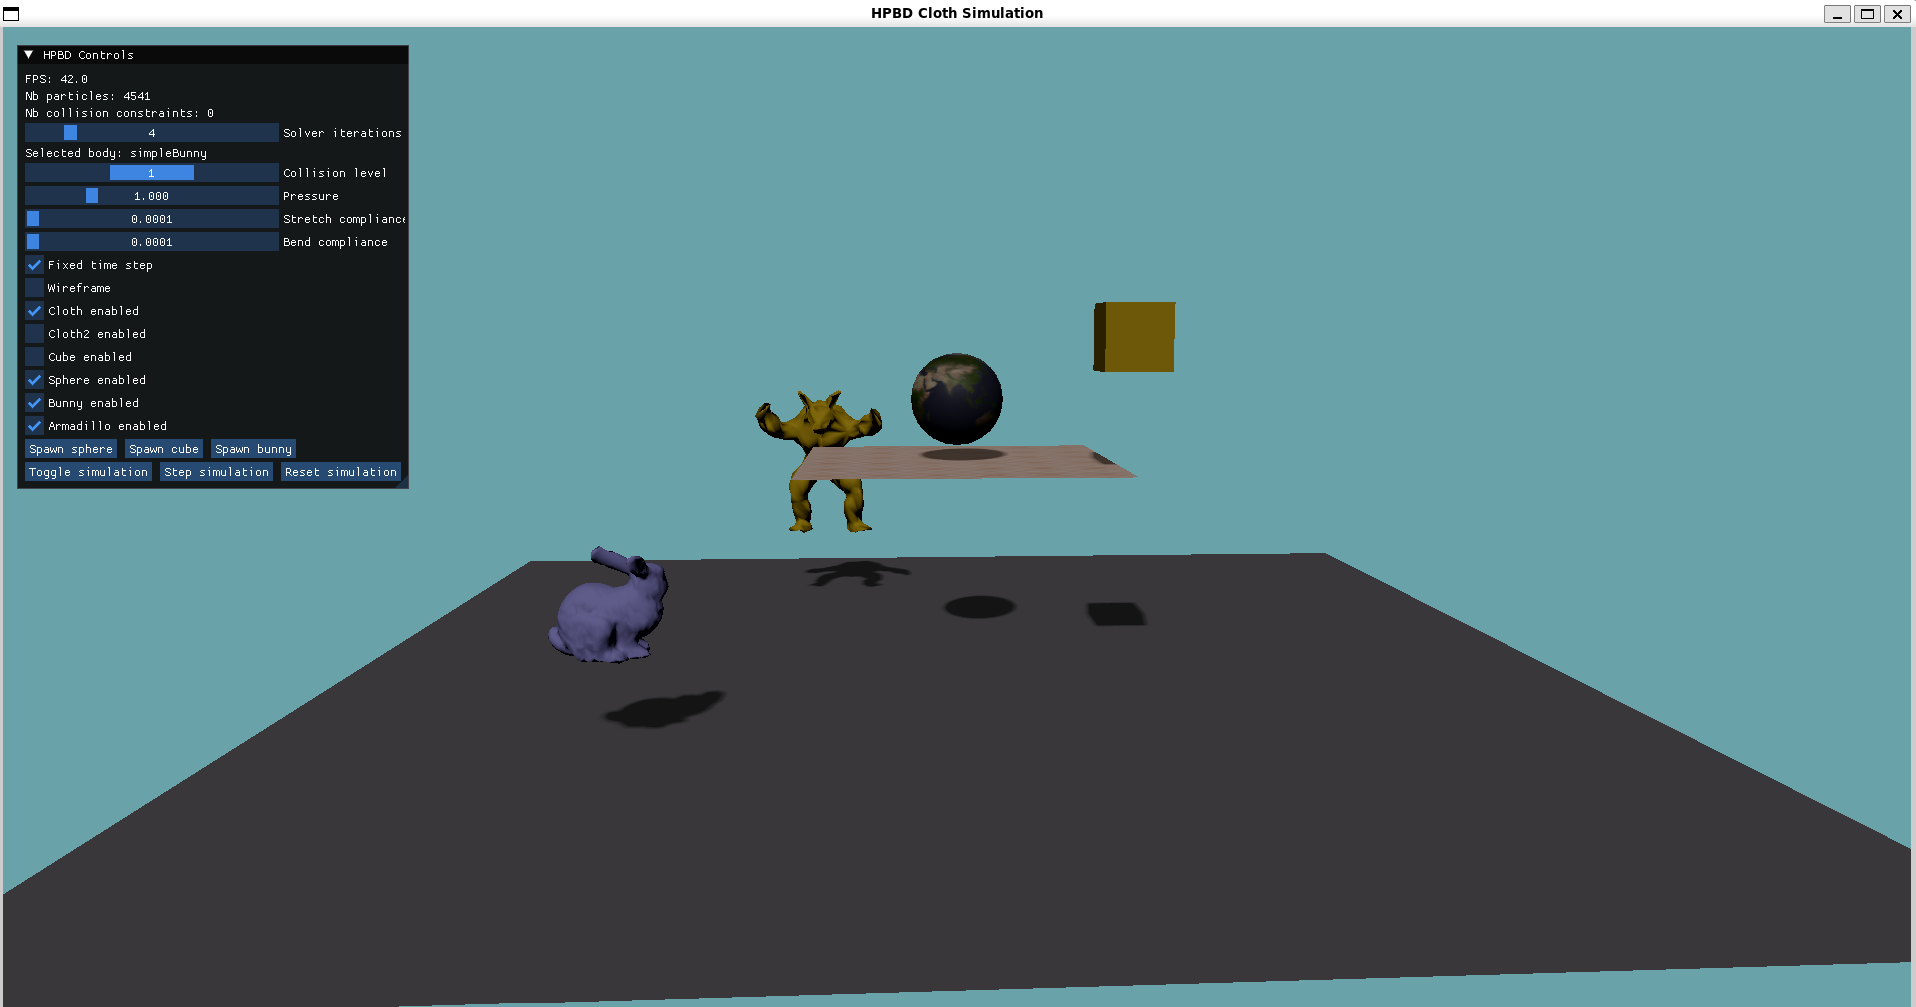
\includegraphics[width=\textwidth]{images/HPBD2.png}
    \caption{Multi-body interaction.}
    \label{fig:hpbd2}
  \end{subfigure}\hfill
  \begin{subfigure}[t]{0.32\textwidth}
    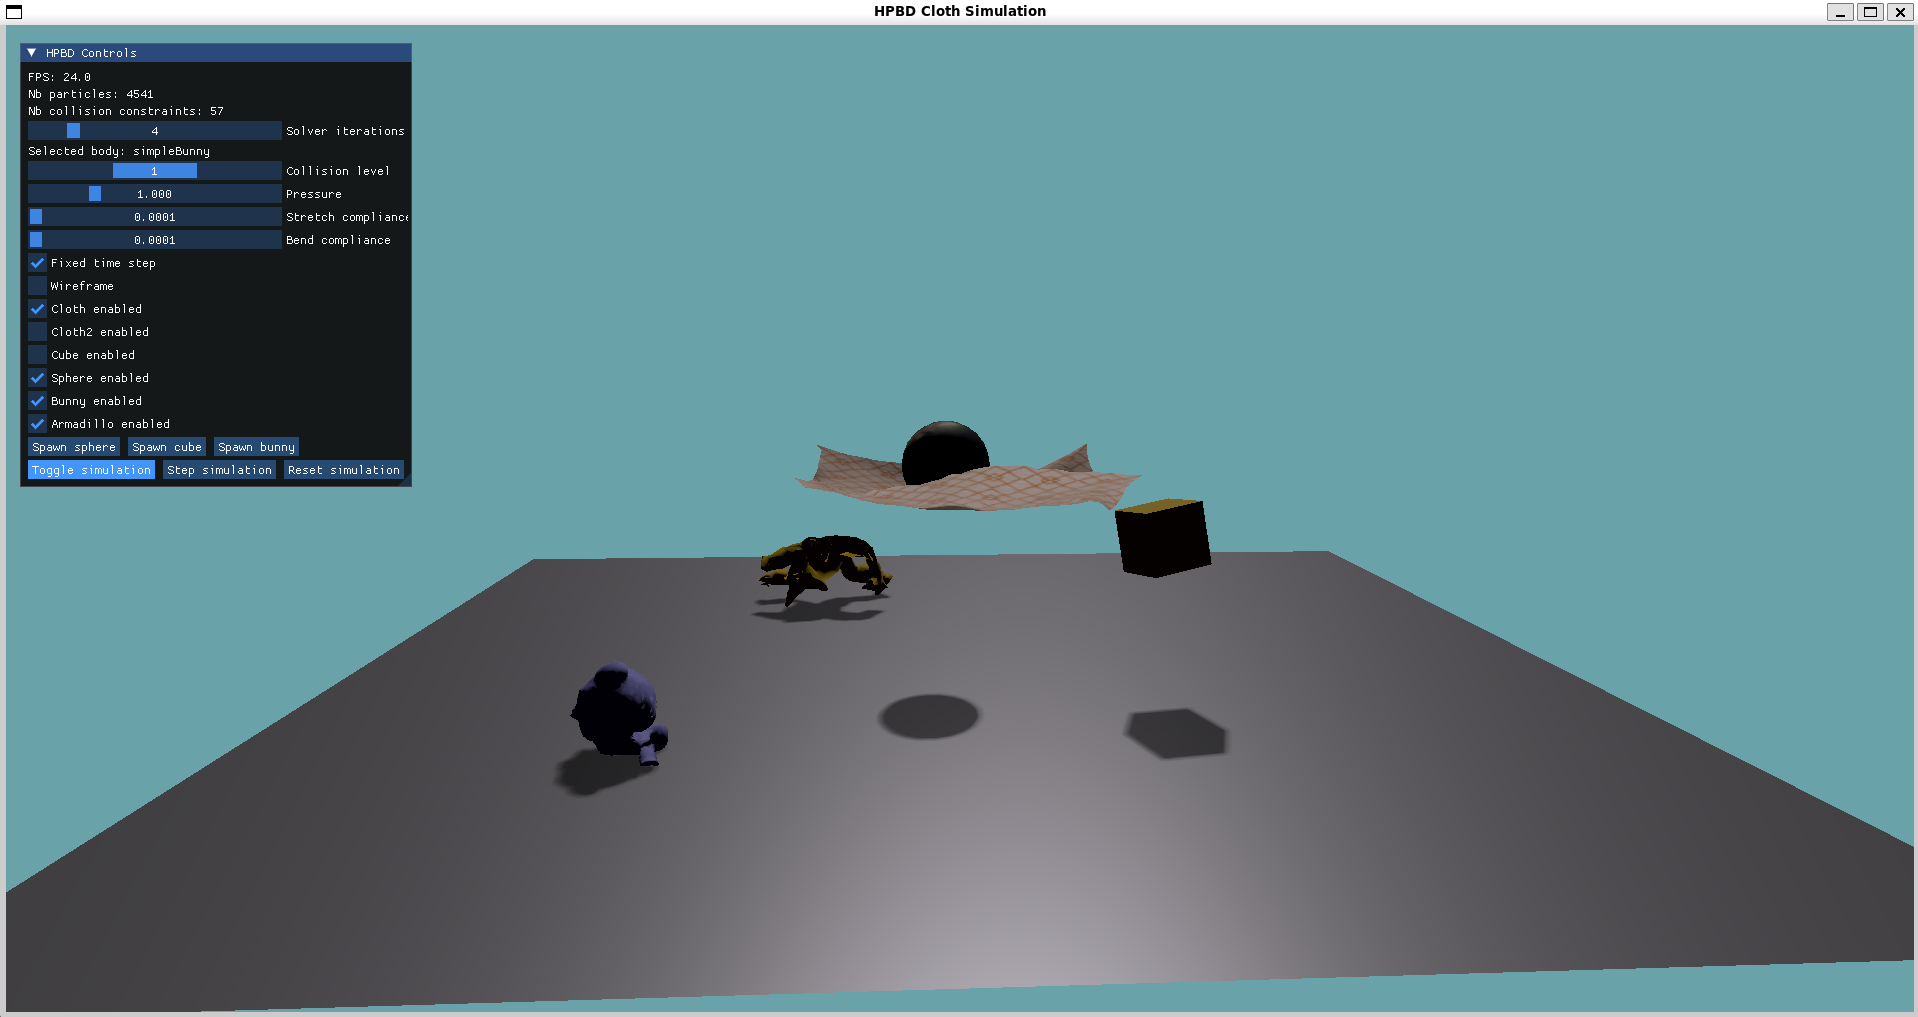
\includegraphics[width=\textwidth]{images/HPBD3.png}
    \caption{Cloth under sphere with shadow mapping.}
    \label{fig:hpbd3}
  \end{subfigure}
  \caption{XPBD cloth simulation with 4{,}541 particles and 4 solver
           iterations across three interaction scenarios.}
  \label{fig:hpbd_results}
\end{figure}

\subsection{Mass-Spring Flag Simulation}

Figures~\ref{fig:cloth1} and~\ref{fig:cloth2} show the cloth flag prototype
evaluating sphere collision and wind response.  The parameter panel exposed
spring constants ($K_0$--$K_2$), damping coefficients ($V_0$--$V_2$), wind
velocity, and sphere radius at runtime.  The cloth correctly draped around
and parted from the sphere as it moved, demonstrating robust contact response
under large deformations without constraint deletion.

\begin{figure}[H]
  \centering
  \begin{subfigure}[t]{0.48\textwidth}
    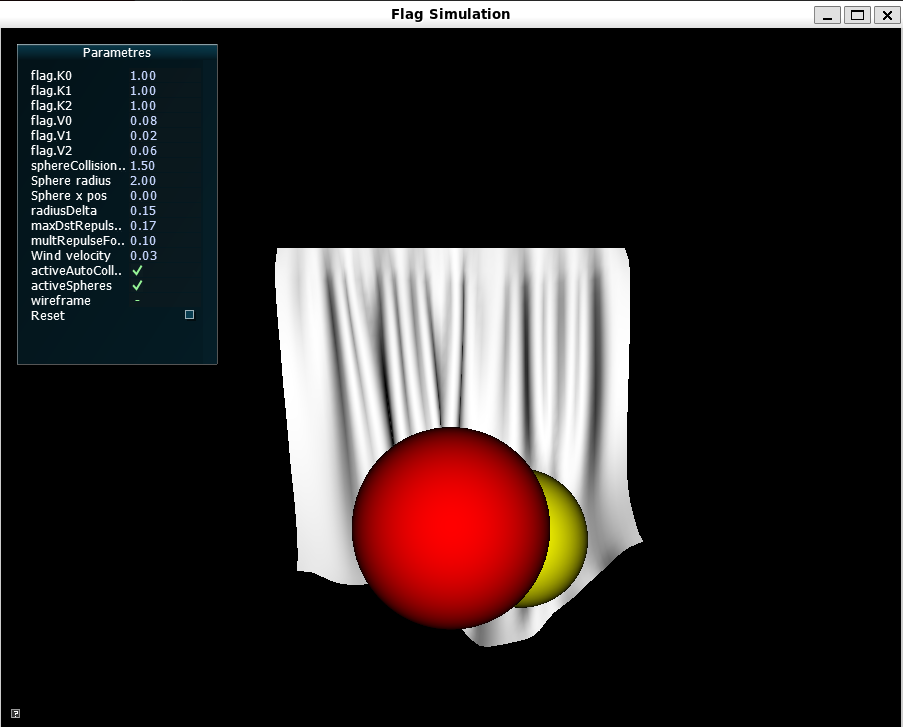
\includegraphics[width=\textwidth]{images/cloth-sim1.png}
    \caption{Cloth draped over two spheres.}
    \label{fig:cloth1}
  \end{subfigure}\hfill
  \begin{subfigure}[t]{0.48\textwidth}
    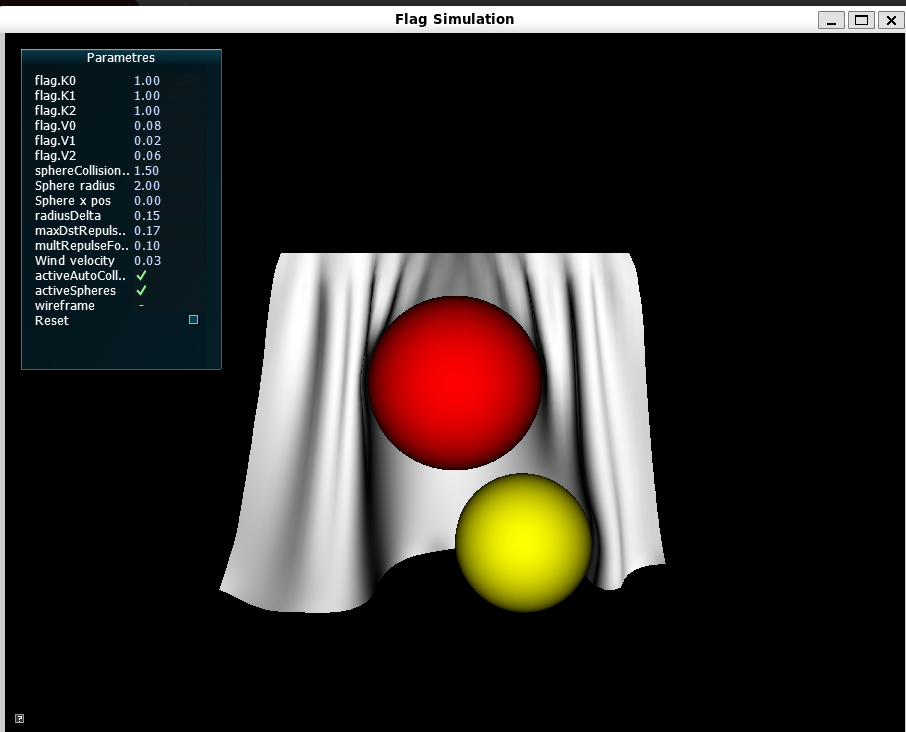
\includegraphics[width=\textwidth]{images/cloth-sim2.png}
    \caption{Cloth bunched by upward sphere motion.}
    \label{fig:cloth2}
  \end{subfigure}
  \caption{Flag cloth prototype showing sphere collision and wind response
           with runtime parameter exposure.}
  \label{fig:cloth_results}
\end{figure}

\subsection{GPU Particle System}

The GPU particle benchmark rendered 100{,}000 particles on an NVIDIA GTX 1650
using OpenGL 4.2 under Mesa.  The terminal output below summarises the
pipeline breakdown.



Figure~\ref{fig:particles} shows the particle cloud at runtime.  The average
frame time of 13.53~ms corresponds to 73.91~FPS over 2{,}321 frames.
Rendering consumed only 0.02~ms because all geometry is resolved to instanced
points; the dominant cost is CPU-side data copy at 1.34~ms, suggesting that
a persistent mapped buffer strategy would reduce this overhead further.

\begin{figure}[H]
  \centering
  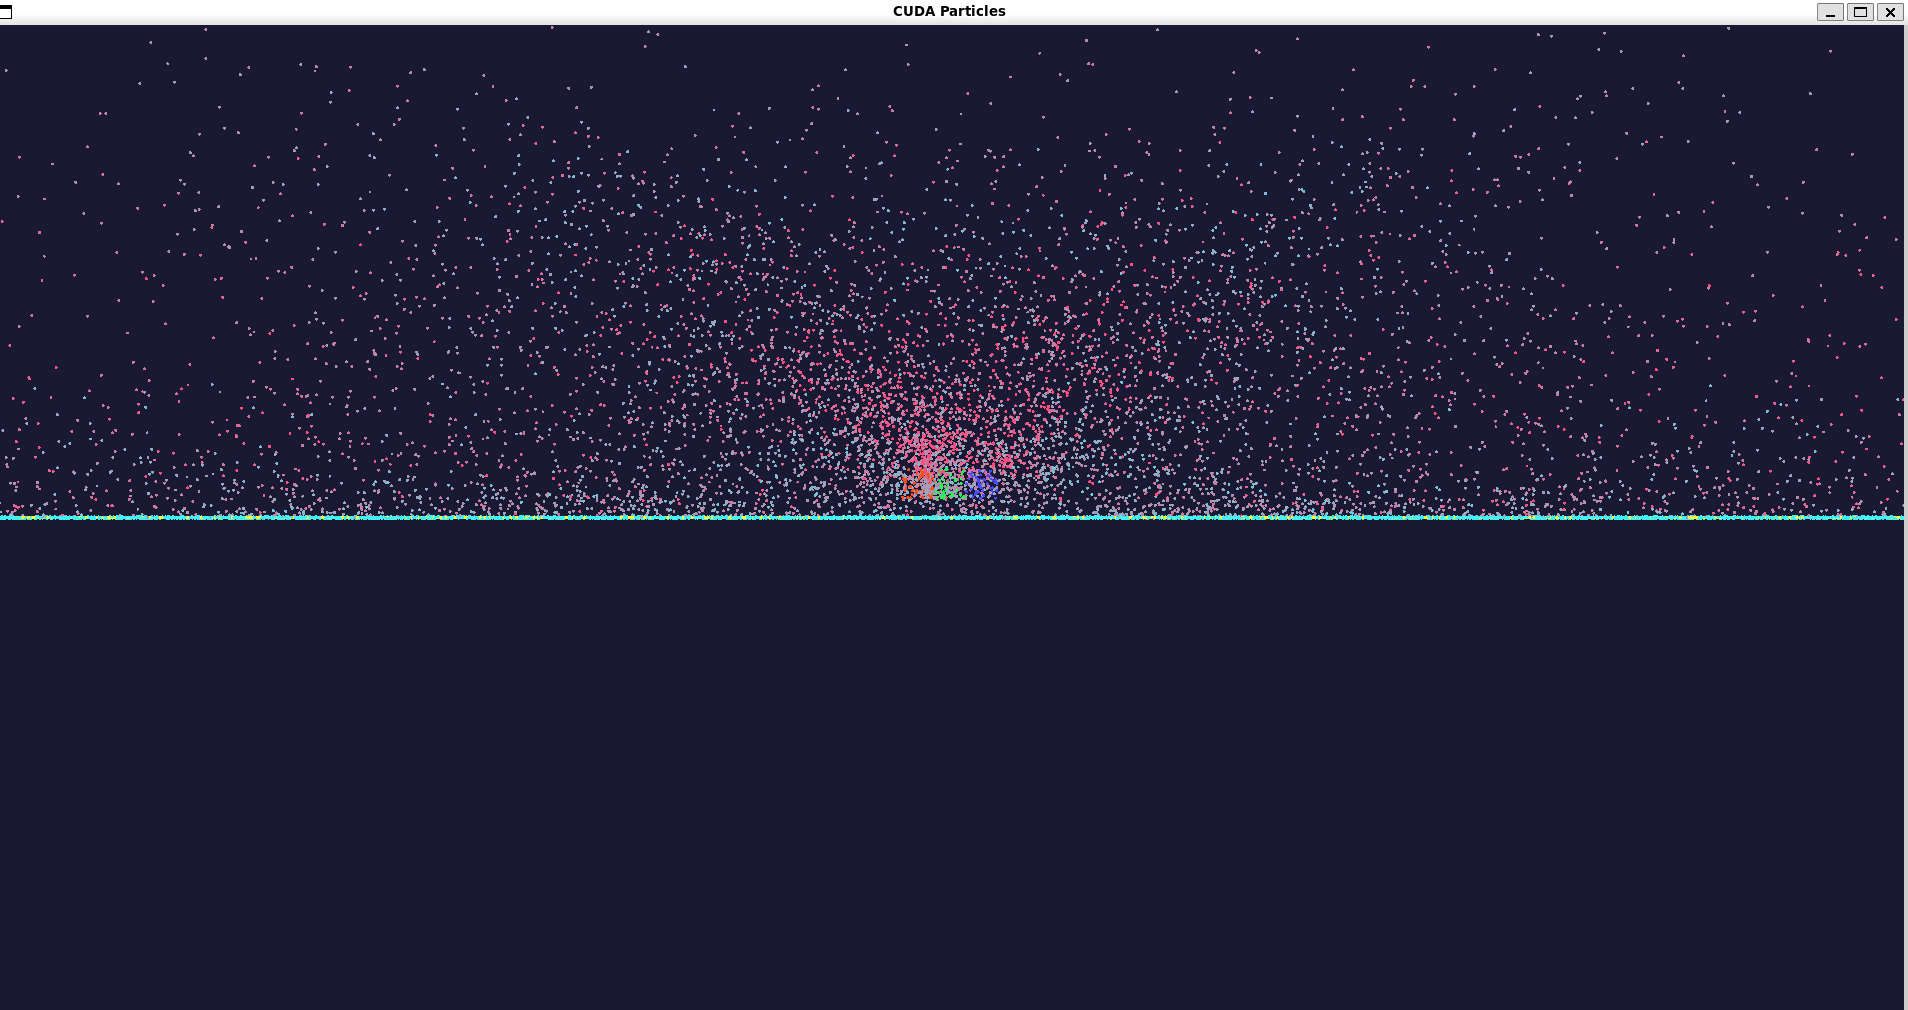
\includegraphics[width=0.85\textwidth]{images/ParticleDemo.png}
  \caption{GPU particle system rendering 100{,}000 particles using cuda at 73.91 average
           FPS on a GTX 1650.}
  \label{fig:particles}
\end{figure}



\subsection{SPH Fluid Demonstration Prototypes}

A standalone 2D SPH fluid demonstration was built to validate the fluid
simulation pipeline and the parameter-driven authoring workflow independently
of the main engine. The demo exposes all SPH parameters (gravity, viscosity,
gas constant, rest density, particle mass, smoothing radius, damping, and
timestep) through runtime sliders and provides four preset fluid types: Water,
Honey, Gas, and Lava. Four scene layouts (Dam Break, Funnel, Beaker, and
Cascade) provide different obstacle configurations.

Figures~\ref{fig:sph_honey}--\ref{fig:sph_water} show the simulation running
across all four fluid types. The Honey preset
(Figure~\ref{fig:sph_honey}) uses high viscosity (1{,}200) and high gravity
(8{,}000) to produce a slow, thick flow that clings to the funnel obstacles.
With 3{,}520 particles the simulation held 33~FPS. The Gas preset
(Figure~\ref{fig:sph_gas}) drops viscosity to 8.0 and raises the gas constant
to 5{,}000, producing dispersed, fast-moving particles that fill the
container volume. Frame rate was 29~FPS at 3{,}520 particles. The Lava preset
(Figure~\ref{fig:sph_lava}) uses the highest gravity (18{,}000) and high rest
density (2{,}000) with moderate viscosity (800), producing a dense, heavy
fluid that pools at the bottom. This was the most expensive configuration at
13~FPS due to the high particle density in the lower region creating more
neighbour interactions. The Water preset on the Beaker scene
(Figure~\ref{fig:sph_water}) shows 2{,}168 particles settling into a
container at 27~FPS with moderate gravity (12{,}000) and viscosity (250).

The key observation across all four presets is that switching fluid types only
changes parameter values. The simulation code, the rendering, and the scene
layout remain identical. This validates the template-driven authoring model:
a teacher can switch between fundamentally different fluid behaviours by
clicking a preset button rather than modifying any code or configuration
files.

\begin{figure}[H]
  \centering
  \begin{subfigure}[t]{0.48\textwidth}
    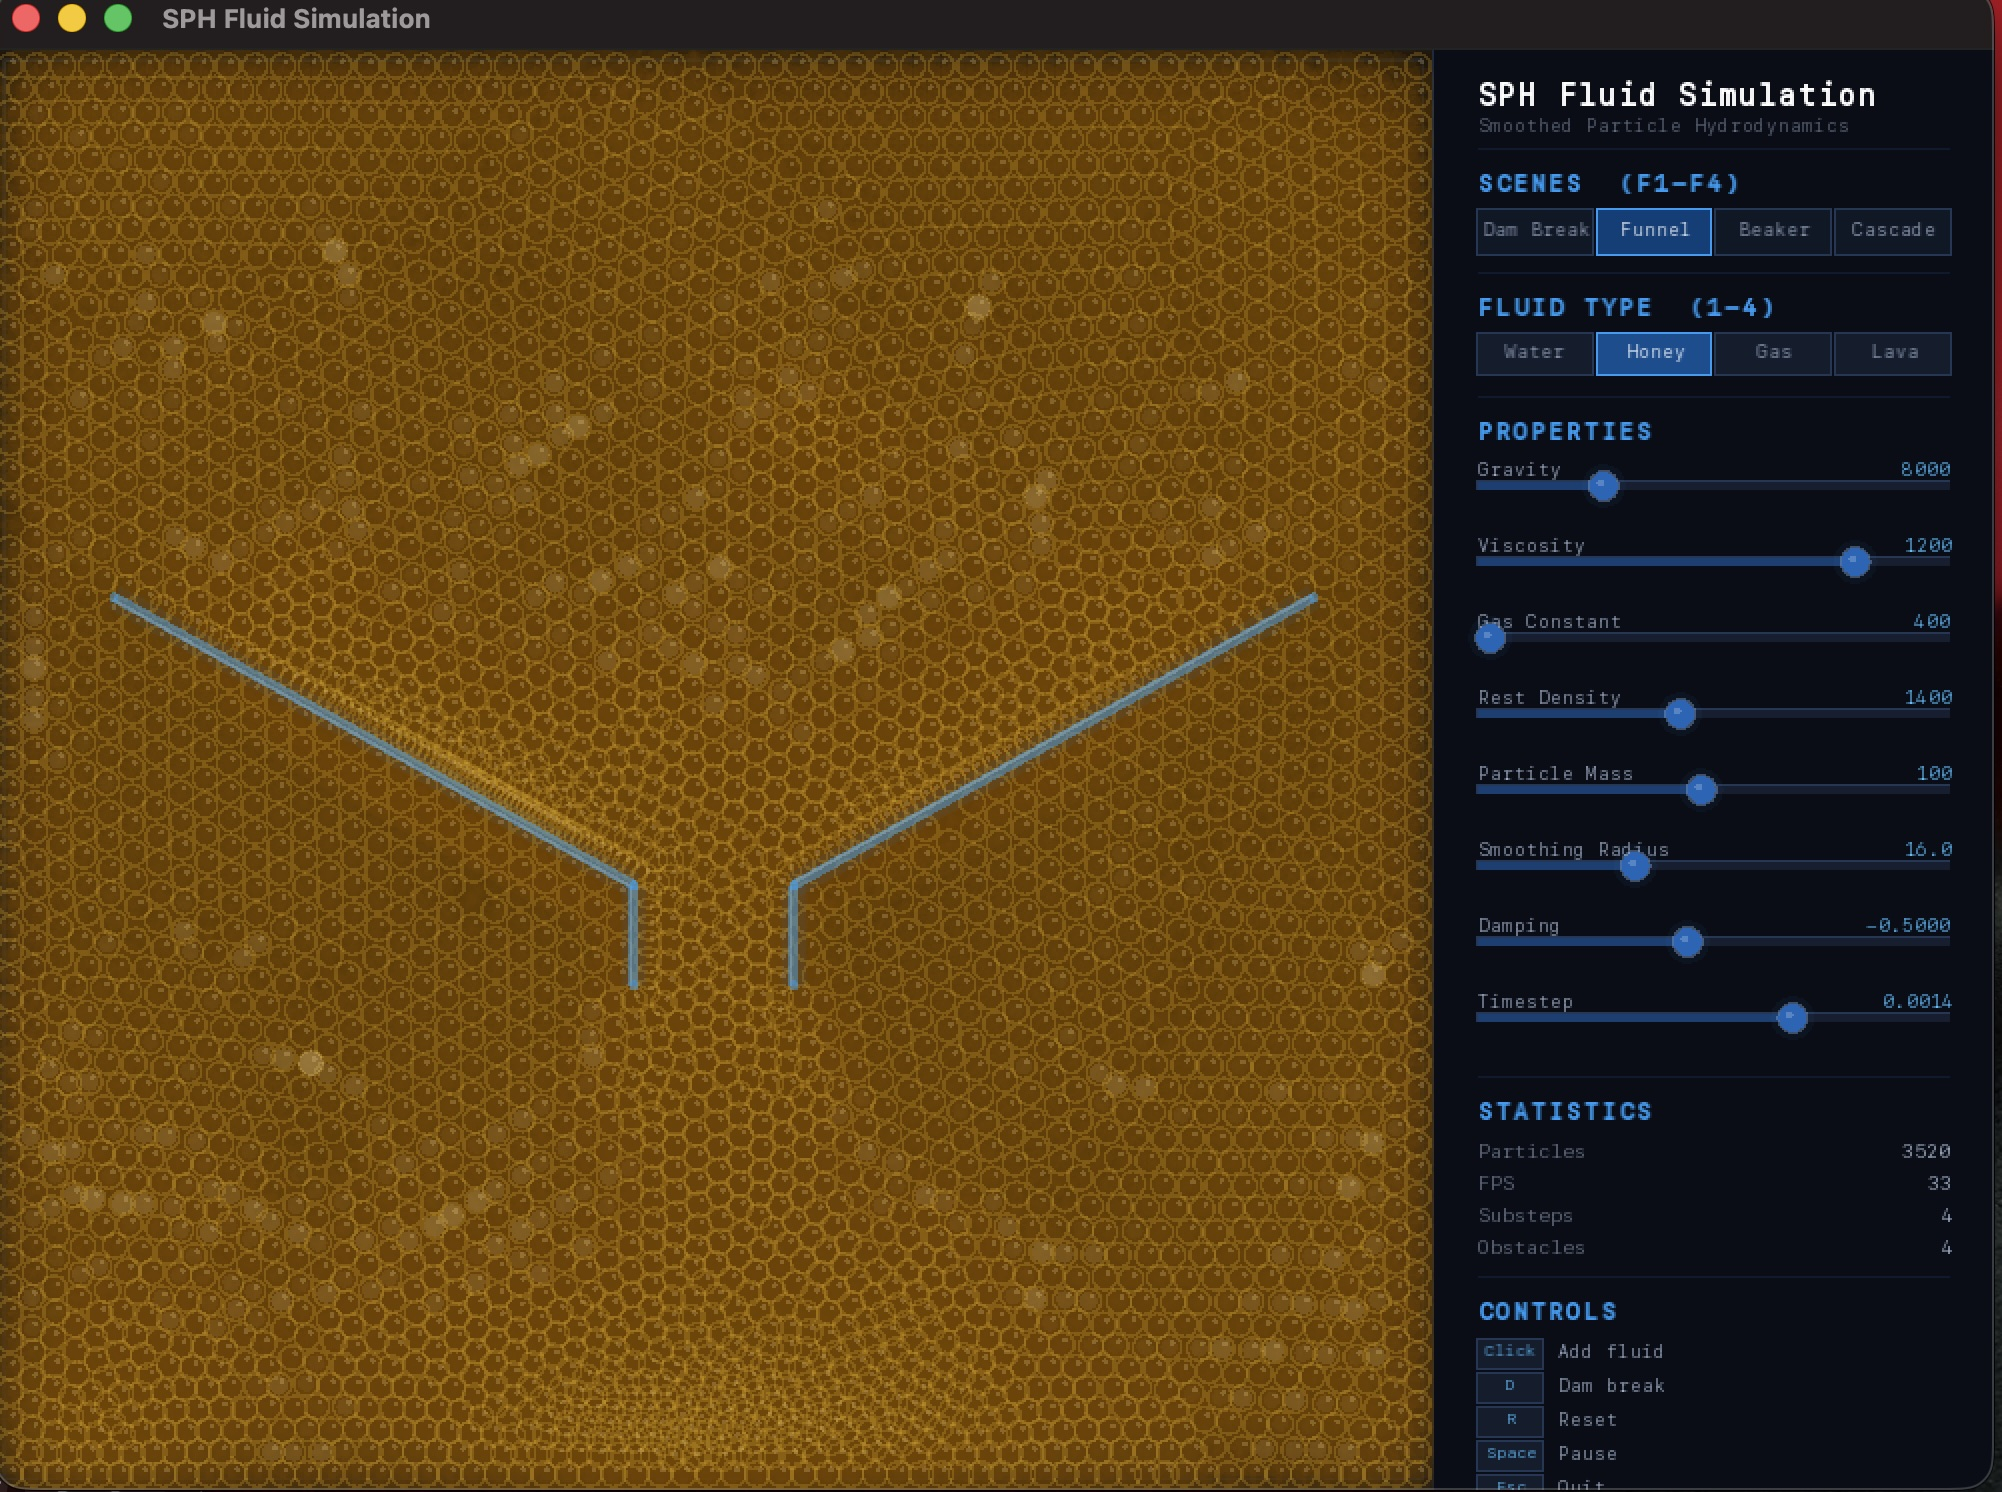
\includegraphics[width=\textwidth]{images/SPH Fluid 1.jpg}
    \caption{Honey preset: viscosity 1{,}200, gravity 8{,}000,
             3{,}520 particles at 33~FPS.}
    \label{fig:sph_honey}
  \end{subfigure}\hfill
  \begin{subfigure}[t]{0.48\textwidth}
    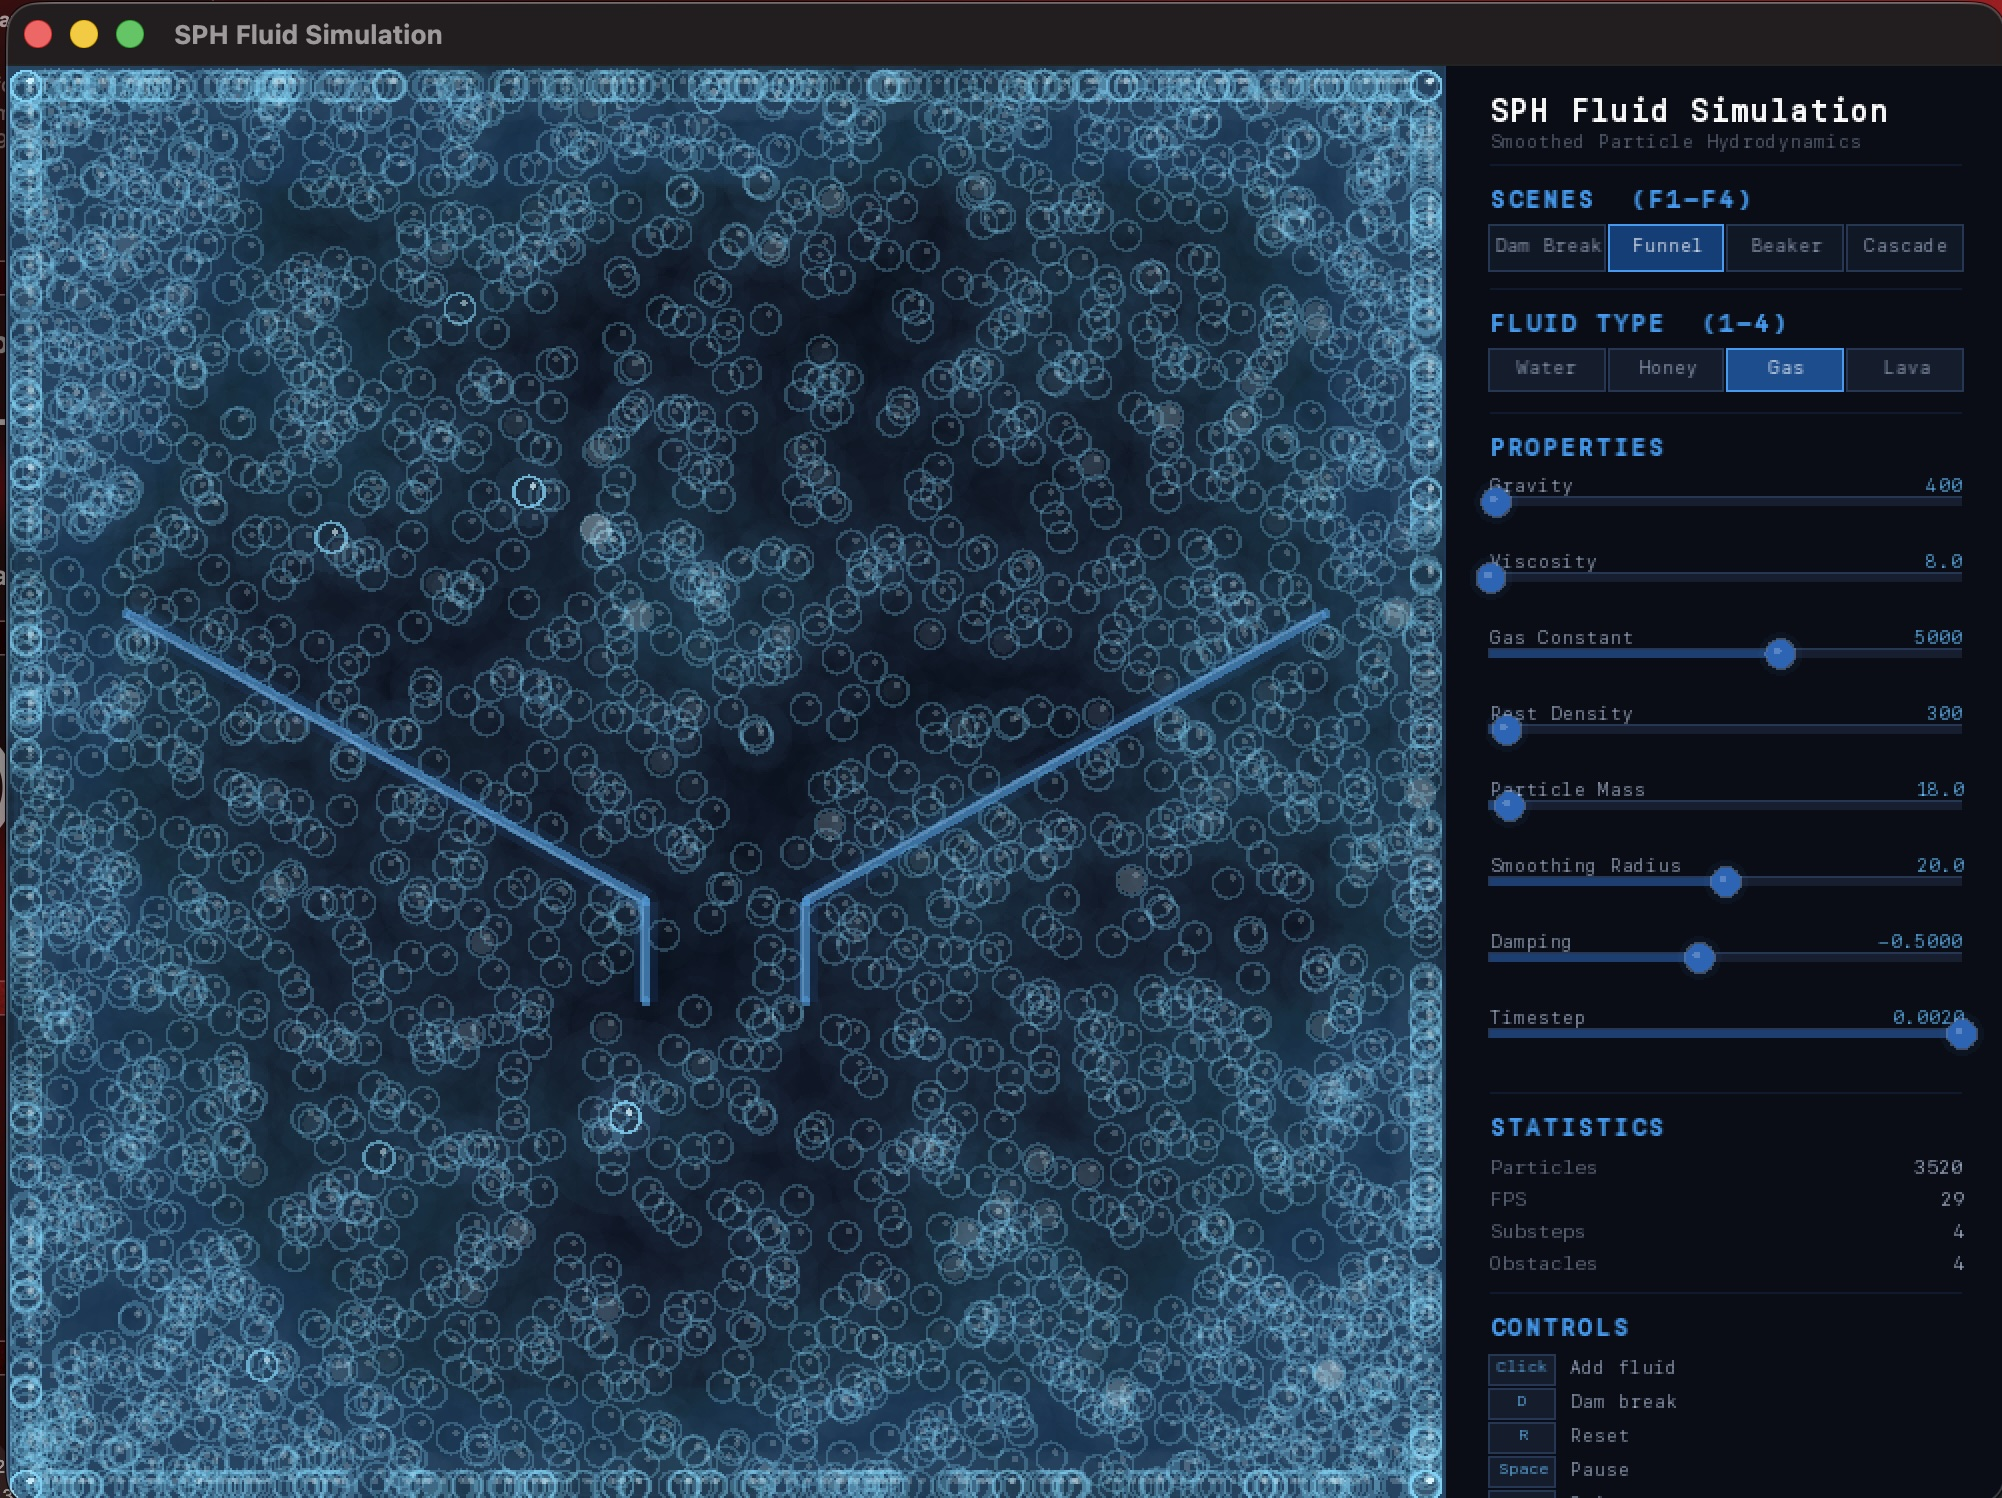
\includegraphics[width=\textwidth]{images/Sph2.jpg}
    \caption{Gas preset: viscosity 8.0, gas constant 5{,}000,
             3{,}520 particles at 29~FPS.}
    \label{fig:sph_gas}
  \end{subfigure}
  \caption{SPH fluid demonstration showing Honey and Gas presets on the
           Funnel scene with runtime parameter exposure.}
  \label{fig:sph_honey_gas}
\end{figure}

\begin{figure}[H]
  \centering
  \begin{subfigure}[t]{0.48\textwidth}
    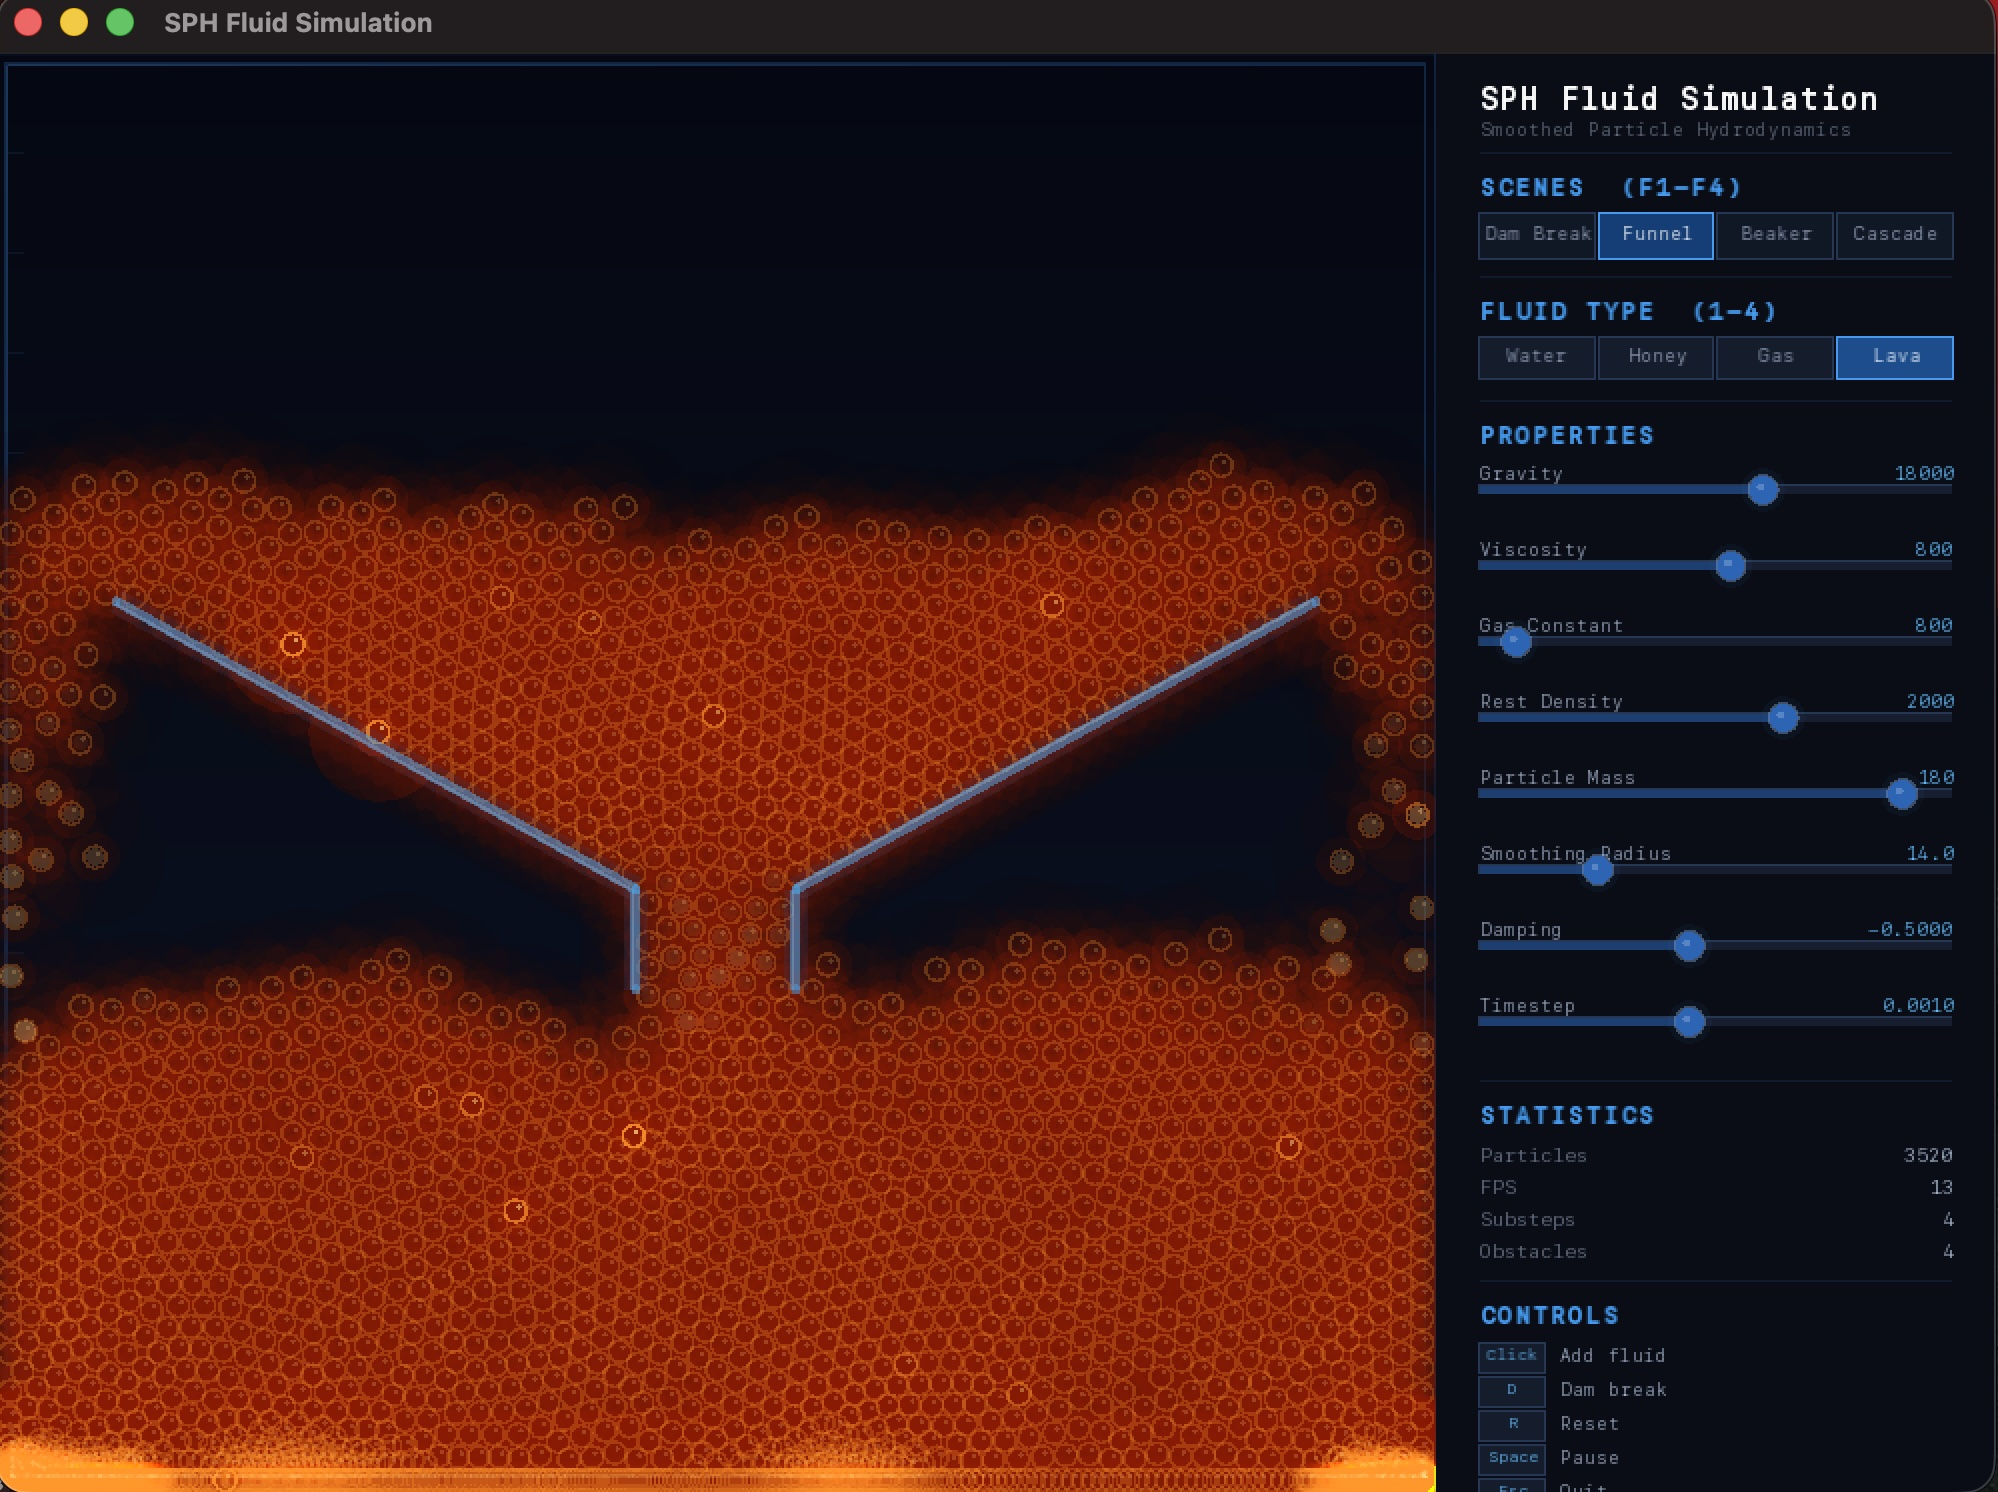
\includegraphics[width=\textwidth]{images/Sph4.jpg}
    \caption{Lava preset: gravity 18{,}000, rest density 2{,}000,
             3{,}520 particles at 13~FPS.}
    \label{fig:sph_lava}
  \end{subfigure}\hfill
  \begin{subfigure}[t]{0.48\textwidth}
    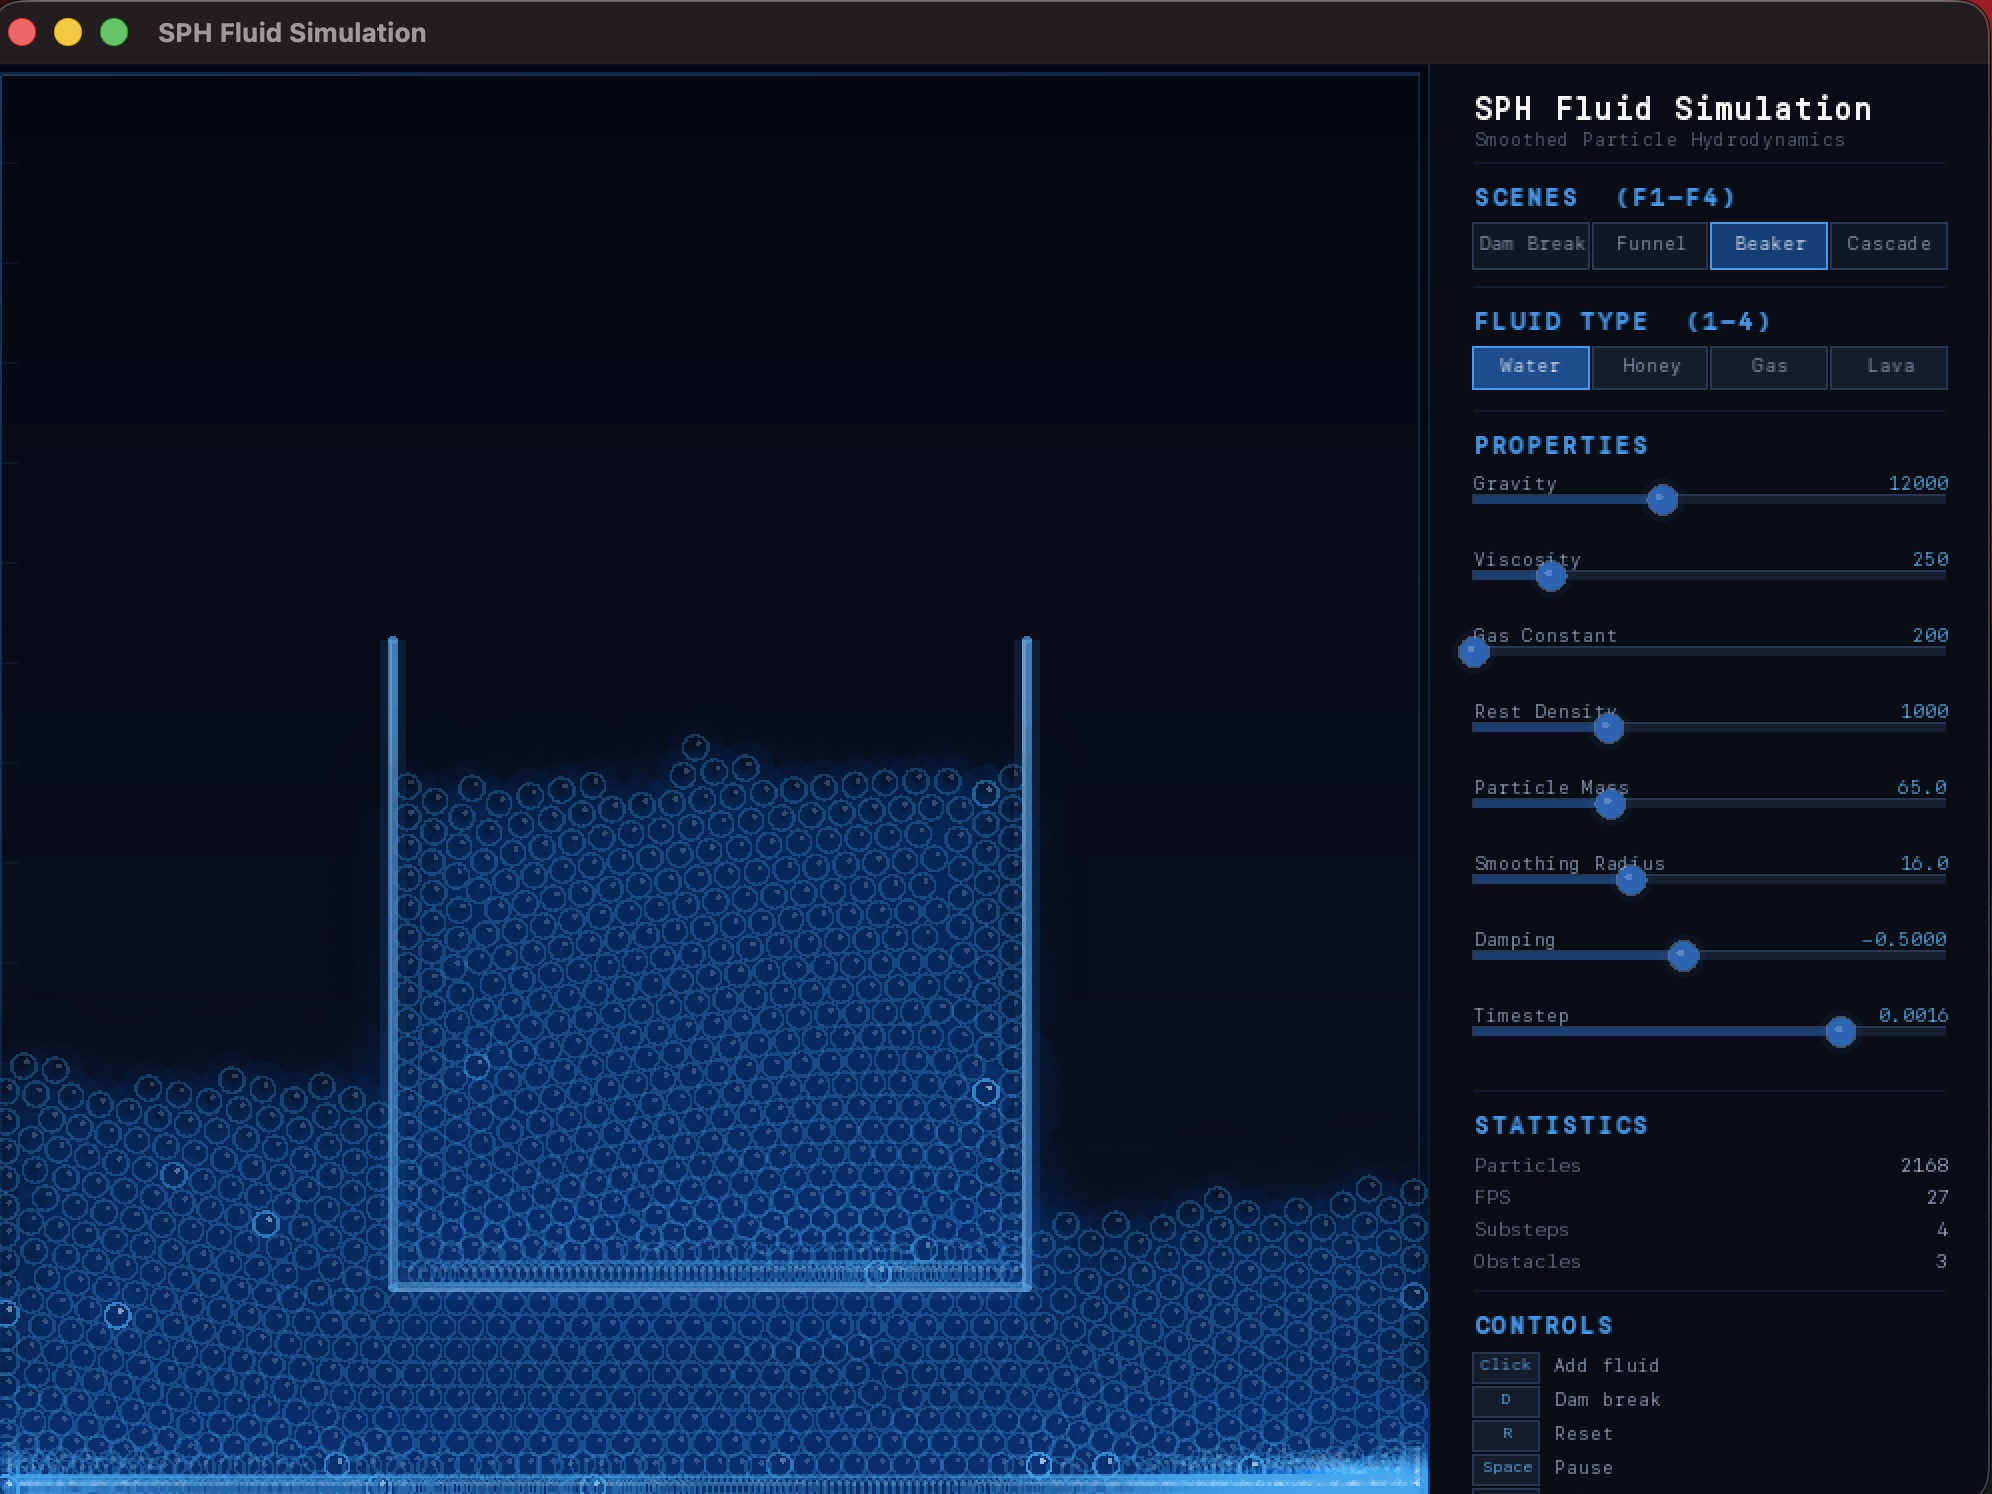
\includegraphics[width=\textwidth]{images/Sph5.jpg}
    \caption{Water preset on Beaker scene: gravity 12{,}000, viscosity 250,
             2{,}168 particles at 27~FPS.}
    \label{fig:sph_water}
  \end{subfigure}
  \caption{SPH fluid demonstration showing Lava and Water presets,
           illustrating the range of fluid behaviours achievable through
           parameter changes alone.}
  \label{fig:sph_lava_water}
\end{figure}



% ═══════════════════════════════════════════════════════════════════════════
\section{Editor Authoring Layer Results}
% ═══════════════════════════════════════════════════════════════════════════

Figures~\ref{fig:editor_welcome}--\ref{fig:editor_rigidbody} document the
educator-facing editor across representative workflows.
Figure~\ref{fig:editor_welcome} shows the WelcomePanel at launch offering
template instantiation, project open, and documentation links.
Figures~\ref{fig:editor_pbr1} and~\ref{fig:editor_pbr2} demonstrate the
deferred PBR viewport with point light placement, material parameter editing,
and the camera preview inset.  Figure~\ref{fig:editor_cloth} shows the
cloth-with-wind preset loaded from PresetManager, with the scene hierarchy
populated automatically.  Figure~\ref{fig:editor_rigidbody} shows the rigid
body stacking preset with the ComponentsWindow exposing mass, damping, body
type, and collider extents without any code interaction.

\begin{figure}[H]
  \centering
  \begin{subfigure}[t]{0.48\textwidth}
    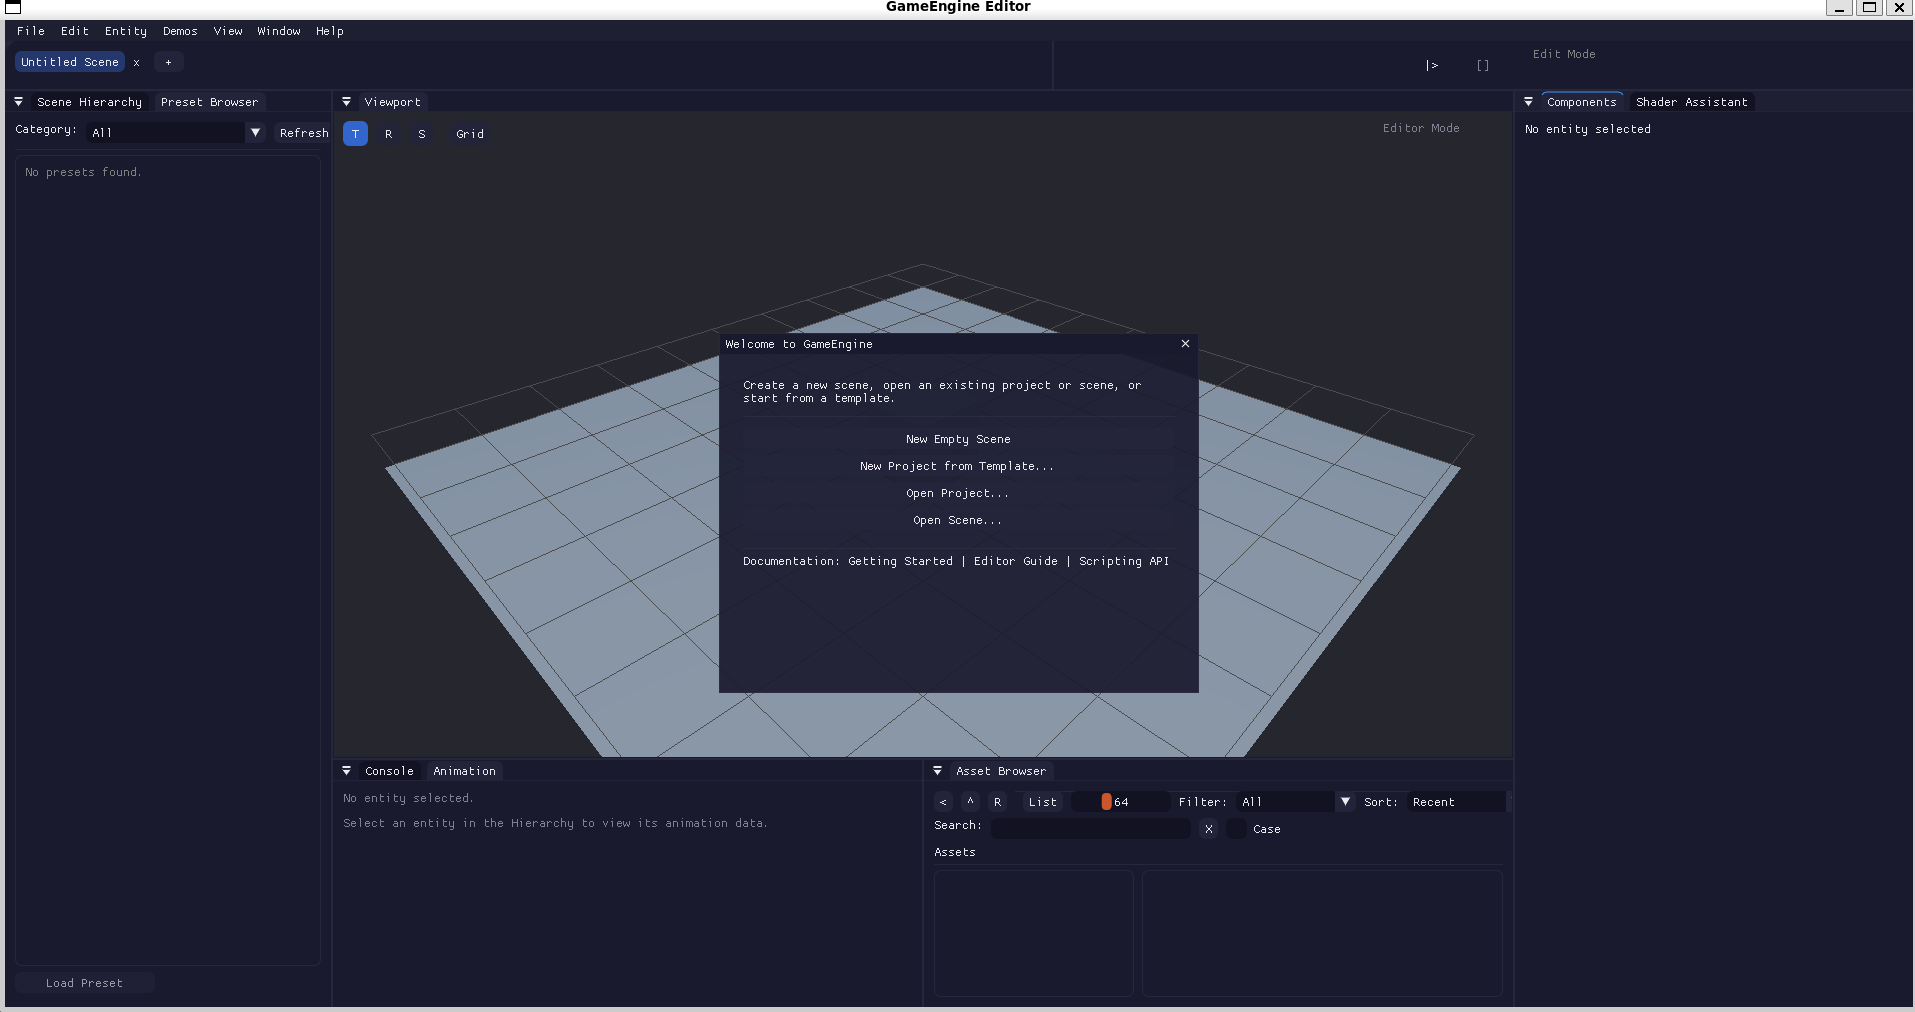
\includegraphics[width=\textwidth]{images/GameEngineEditor.png}
    \caption{WelcomePanel and template selector at launch.}
    \label{fig:editor_welcome}
  \end{subfigure}\hfill
  \begin{subfigure}[t]{0.48\textwidth}
    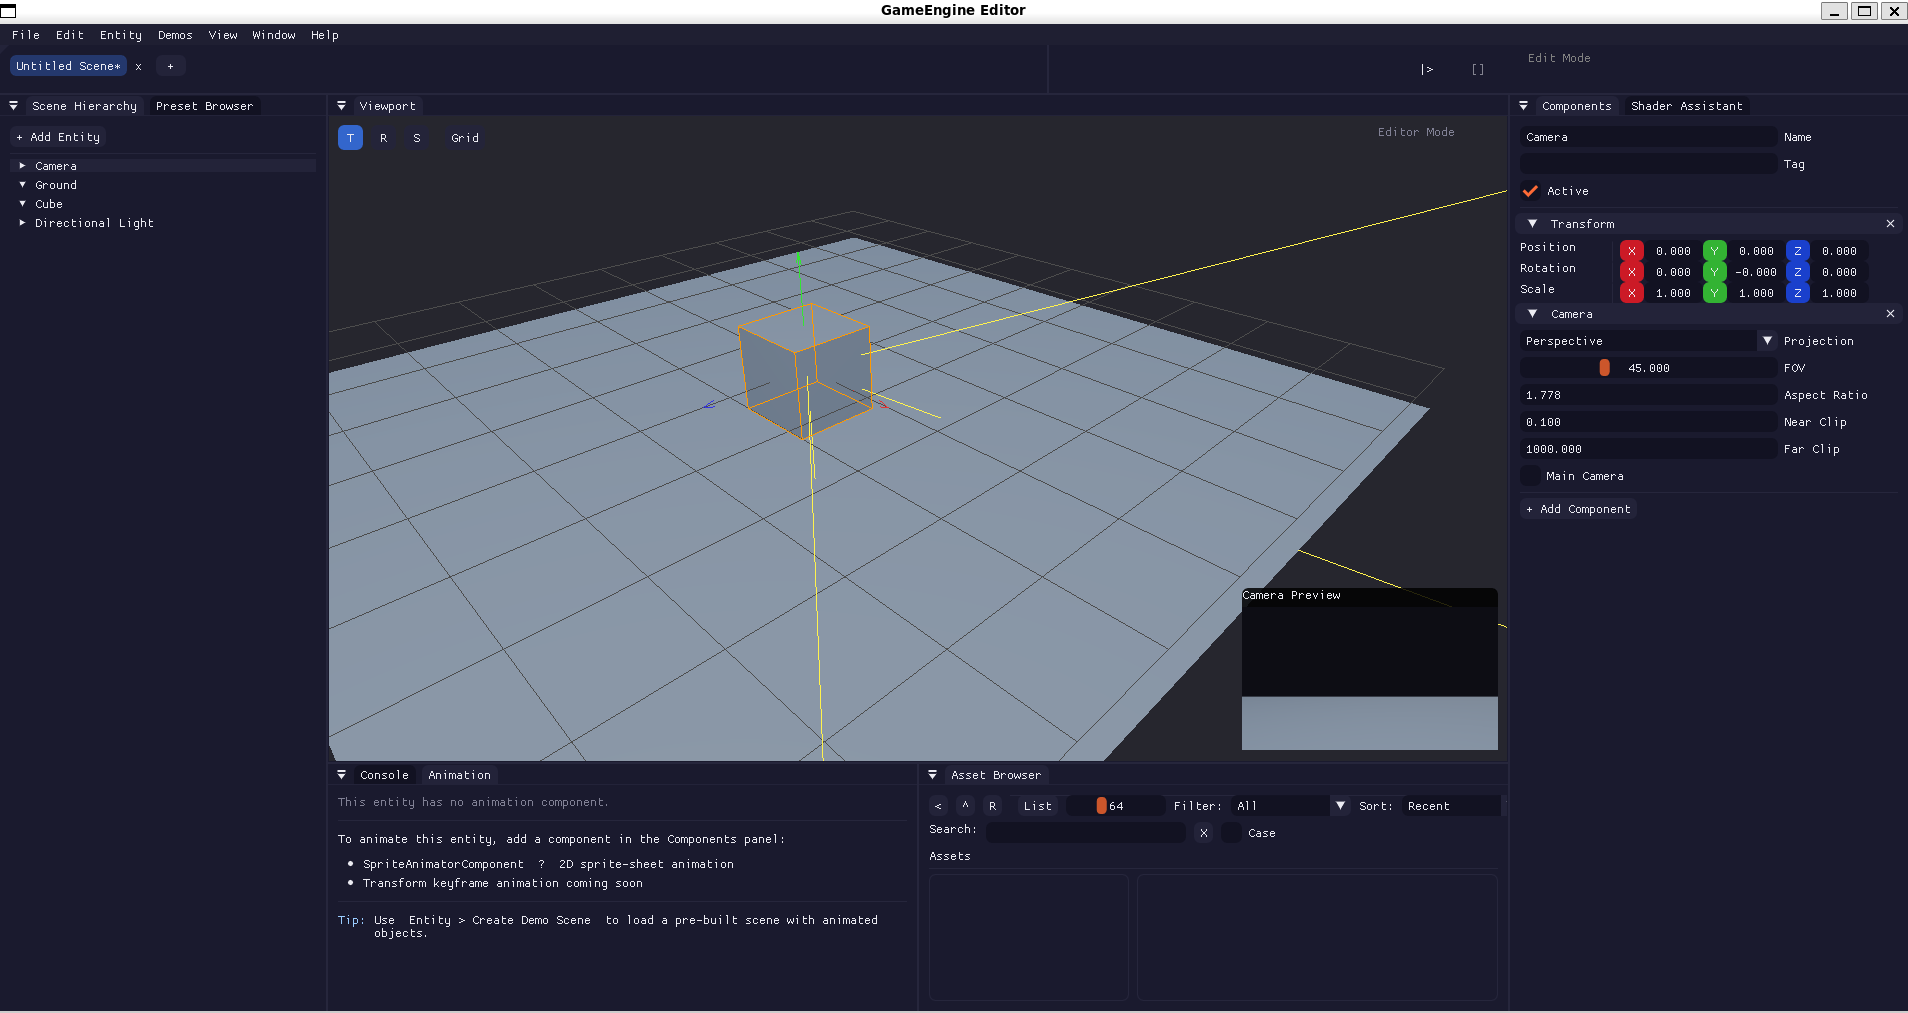
\includegraphics[width=\textwidth]{images/Editor2.png}
    \caption{PBR viewport with camera component inspector.}
    \label{fig:editor_pbr1}
  \end{subfigure}
  \caption{Editor startup and scene authoring workflow.}
\end{figure}

\begin{figure}[H]
  \centering
  \begin{subfigure}[t]{0.32\textwidth}
    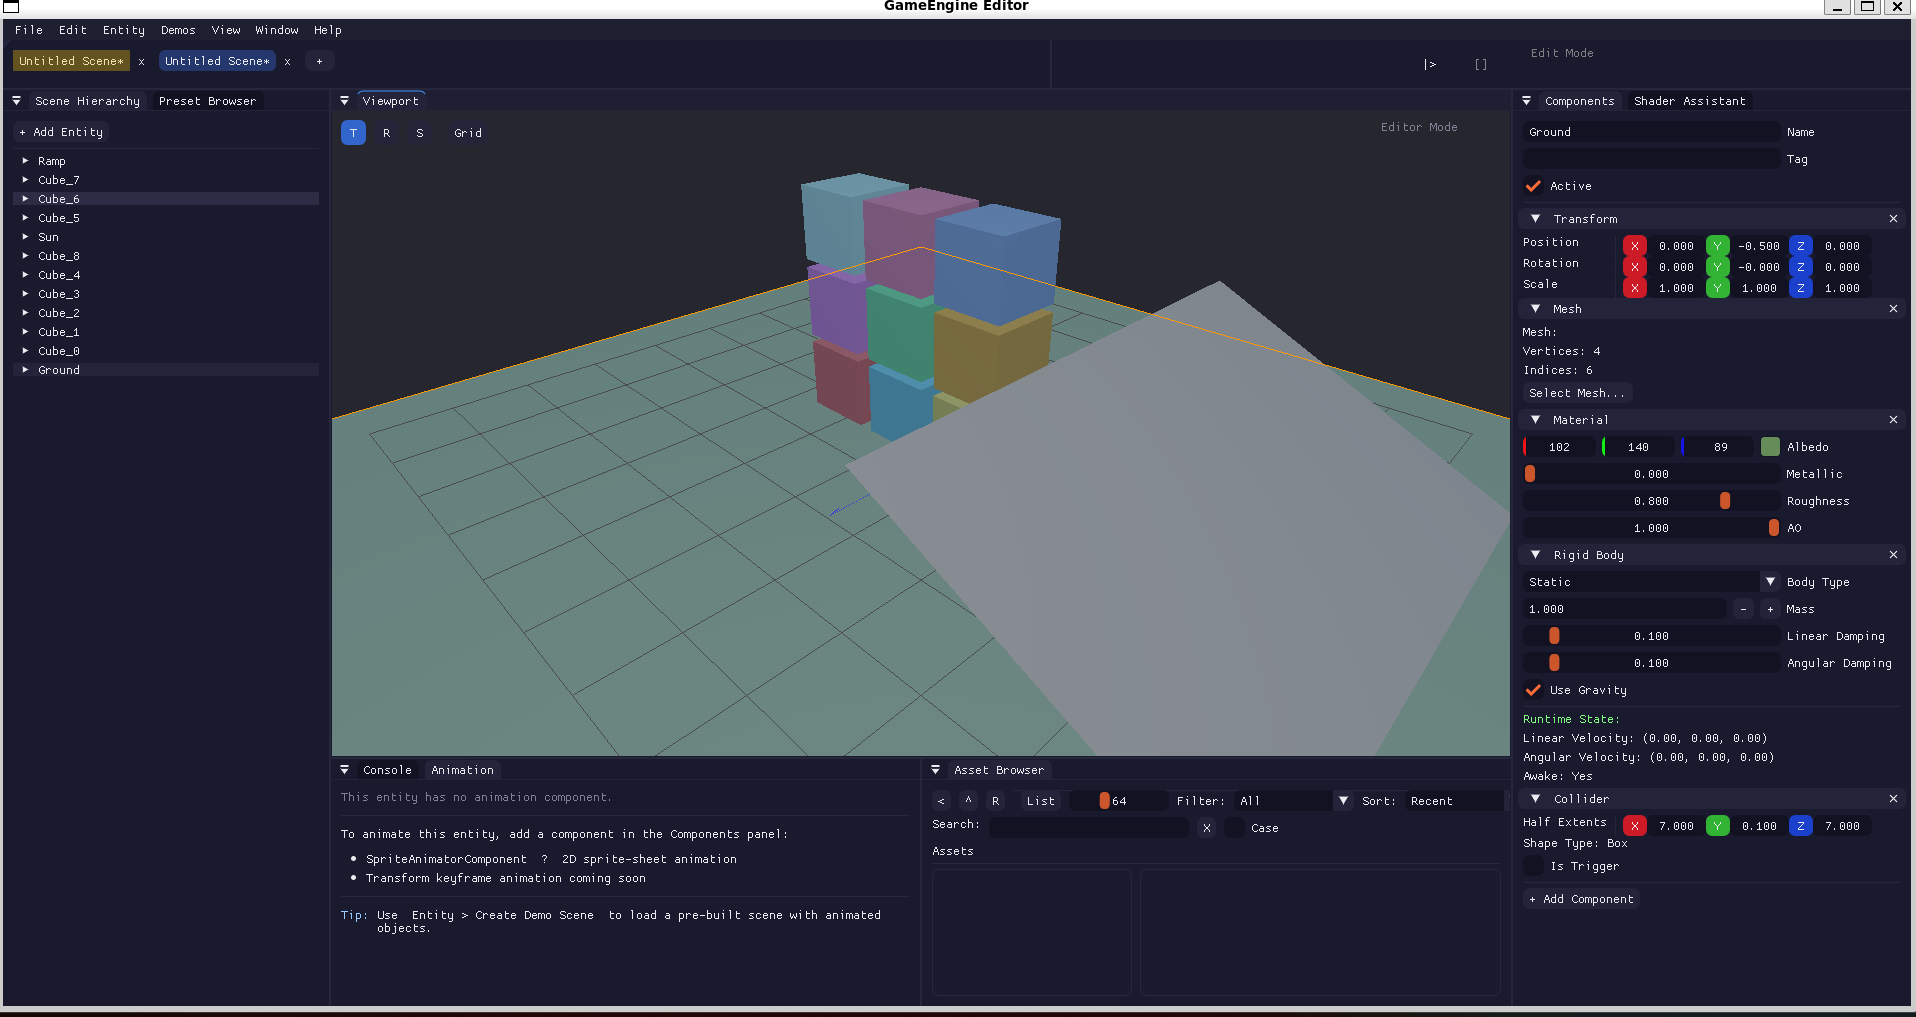
\includegraphics[width=\textwidth]{images/Editor3.png}
    \caption{Deferred PBR with point lights.}
    \label{fig:editor_pbr2}
  \end{subfigure}\hfill
  \begin{subfigure}[t]{0.32\textwidth}
    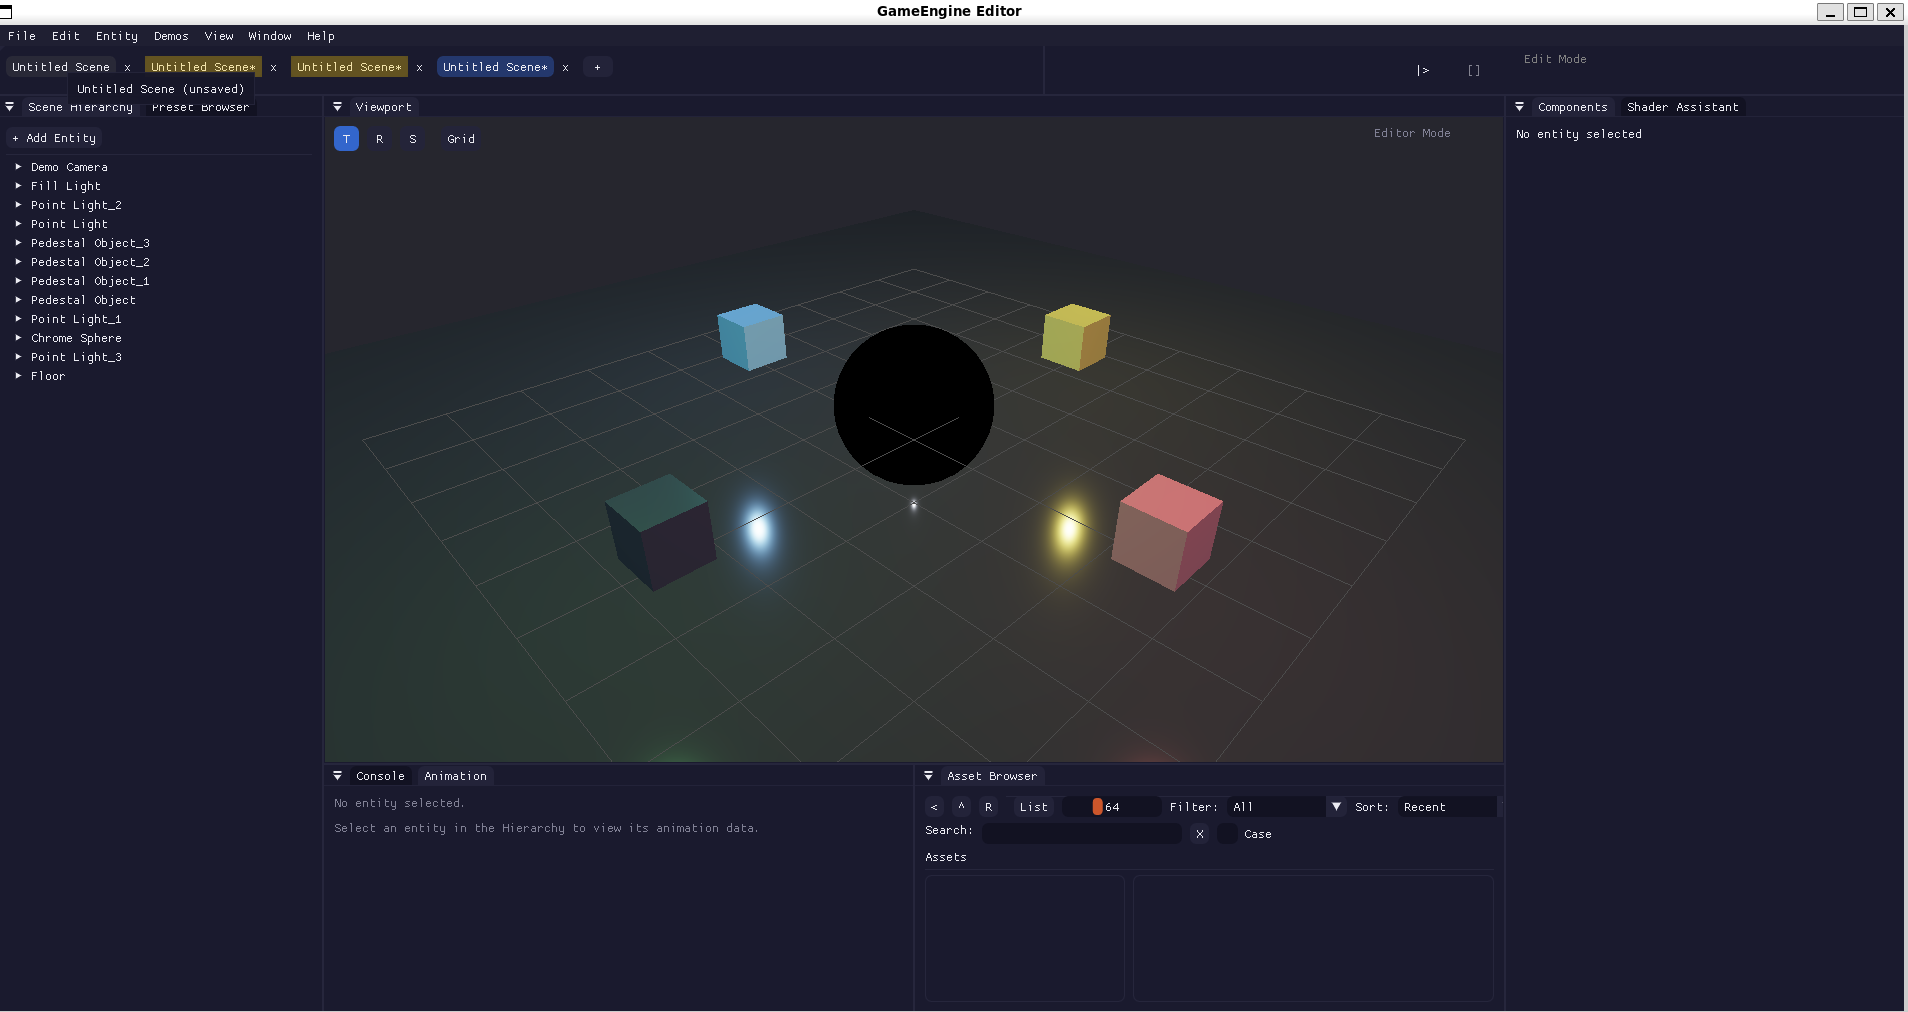
\includegraphics[width=\textwidth]{images/Editor4.png}
    \caption{Cloth preset with hierarchy.}
    \label{fig:editor_cloth}
  \end{subfigure}\hfill
  \begin{subfigure}[t]{0.32\textwidth}
    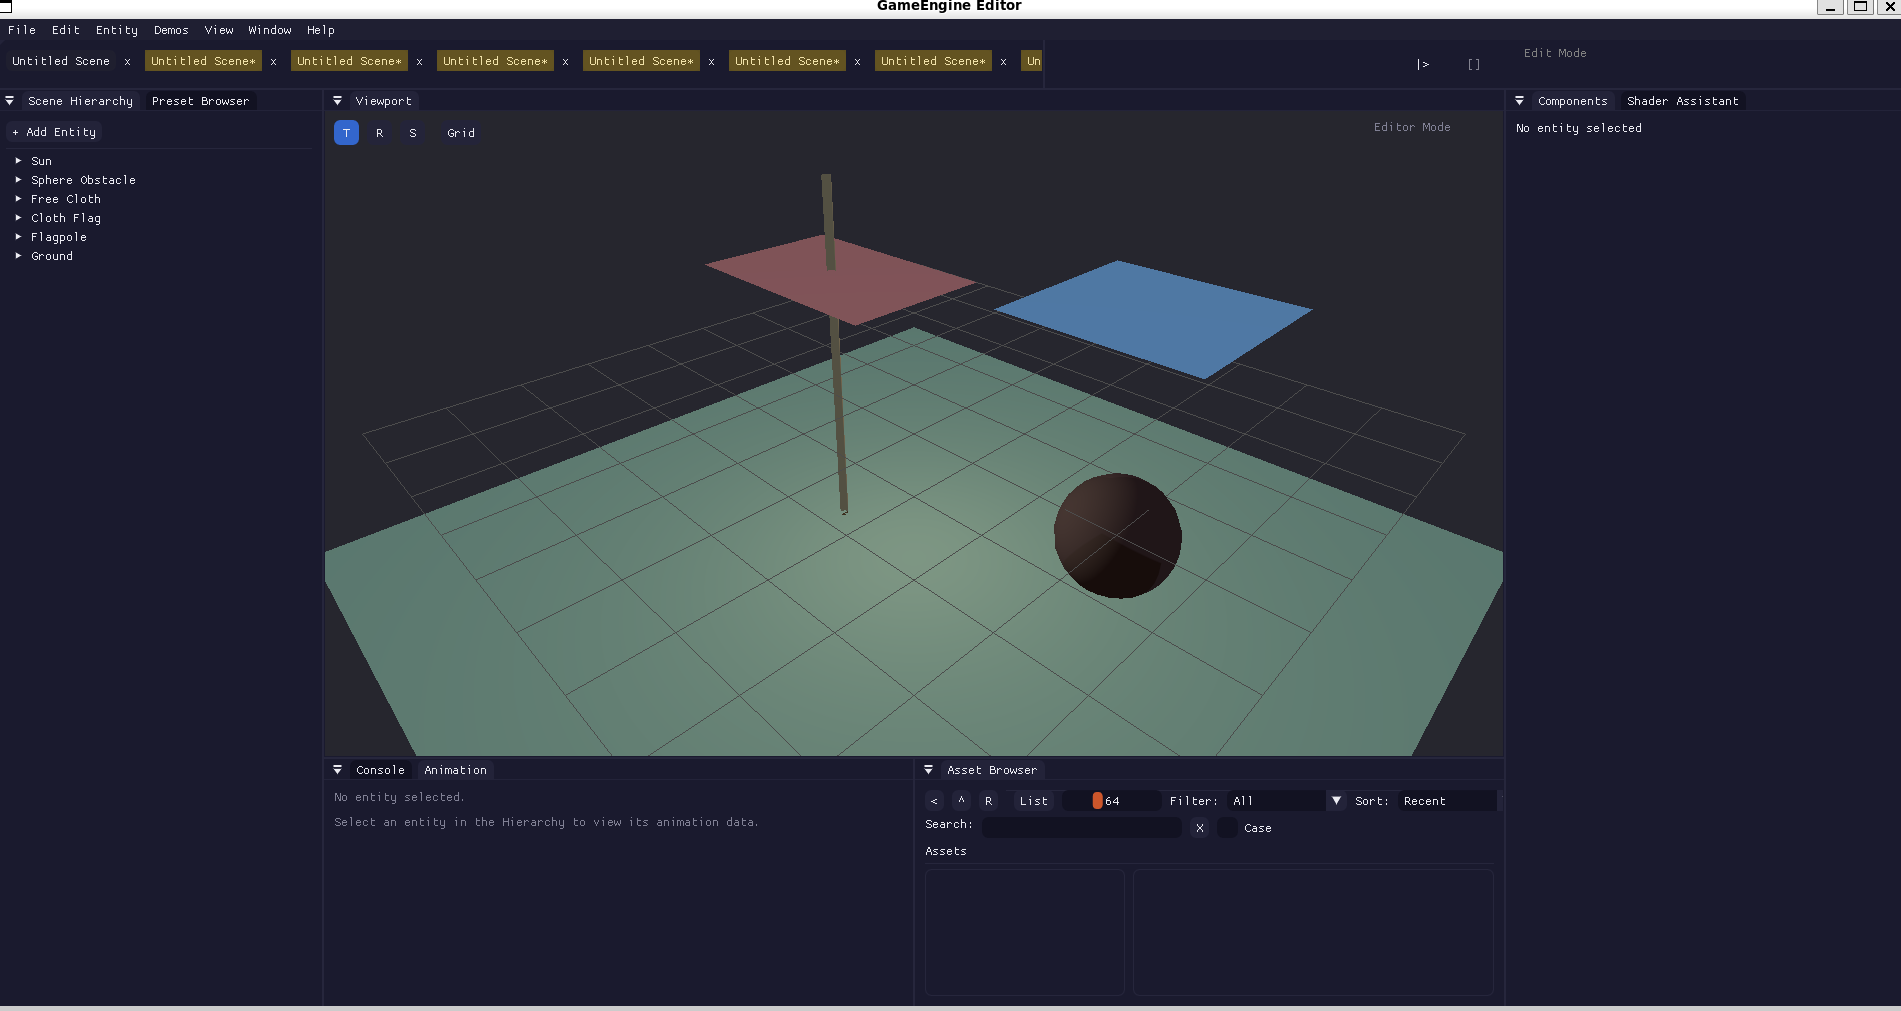
\includegraphics[width=\textwidth]{images/Editor6.png}
    \caption{Rigid body stacking with inspector.}
    \label{fig:editor_rigidbody}
  \end{subfigure}
  \caption{Editor scenes showing template-instantiated demonstrations with
           component inspection and no code exposure.}
  \label{fig:editor_scenes}
\end{figure}


\subsection{Natural Language Shader Generation}

The shader generator was evaluated on two representative prompts to
demonstrate the natural language authoring workflow. Given the prompt
\texttt{--use "Mandelbrot"}, the system produced a complete GLSL fragment
shader implementing the Mandelbrot set with animated colour cycling driven
by a \texttt{time} uniform. Figures~\ref{fig:shader_mandelbrot_code}
and~\ref{fig:shader_mandelbrot_preview} show the generated source and the
live preview respectively. The shader correctly implements the escape-time
algorithm with 100 iterations, maps the iteration count to a sinusoidal
RGB colour triple, and renders the set boundary with smooth animated colour
variation at interactive frame rates under OpenGL 4.1.

Given the prompt \texttt{--use "Fire"}, the system generated a noise-based
animated fire fragment shader using a hash function and layered smooth-noise
octaves to simulate flame movement. Figure~\ref{fig:shader_fire} shows the
live preview alongside the generated vertex and fragment shader source. The
system reported zero repair attempts for both shaders, indicating that the
generated GLSL compiled without errors on the first attempt. Both outputs
were saved to \texttt{output/generated.vert} and
\texttt{output/generated.frag} and applied to scene geometry within the
engine editor without manual modification.

\begin{figure}[H]
  \centering
  \begin{subfigure}[t]{0.48\textwidth}
    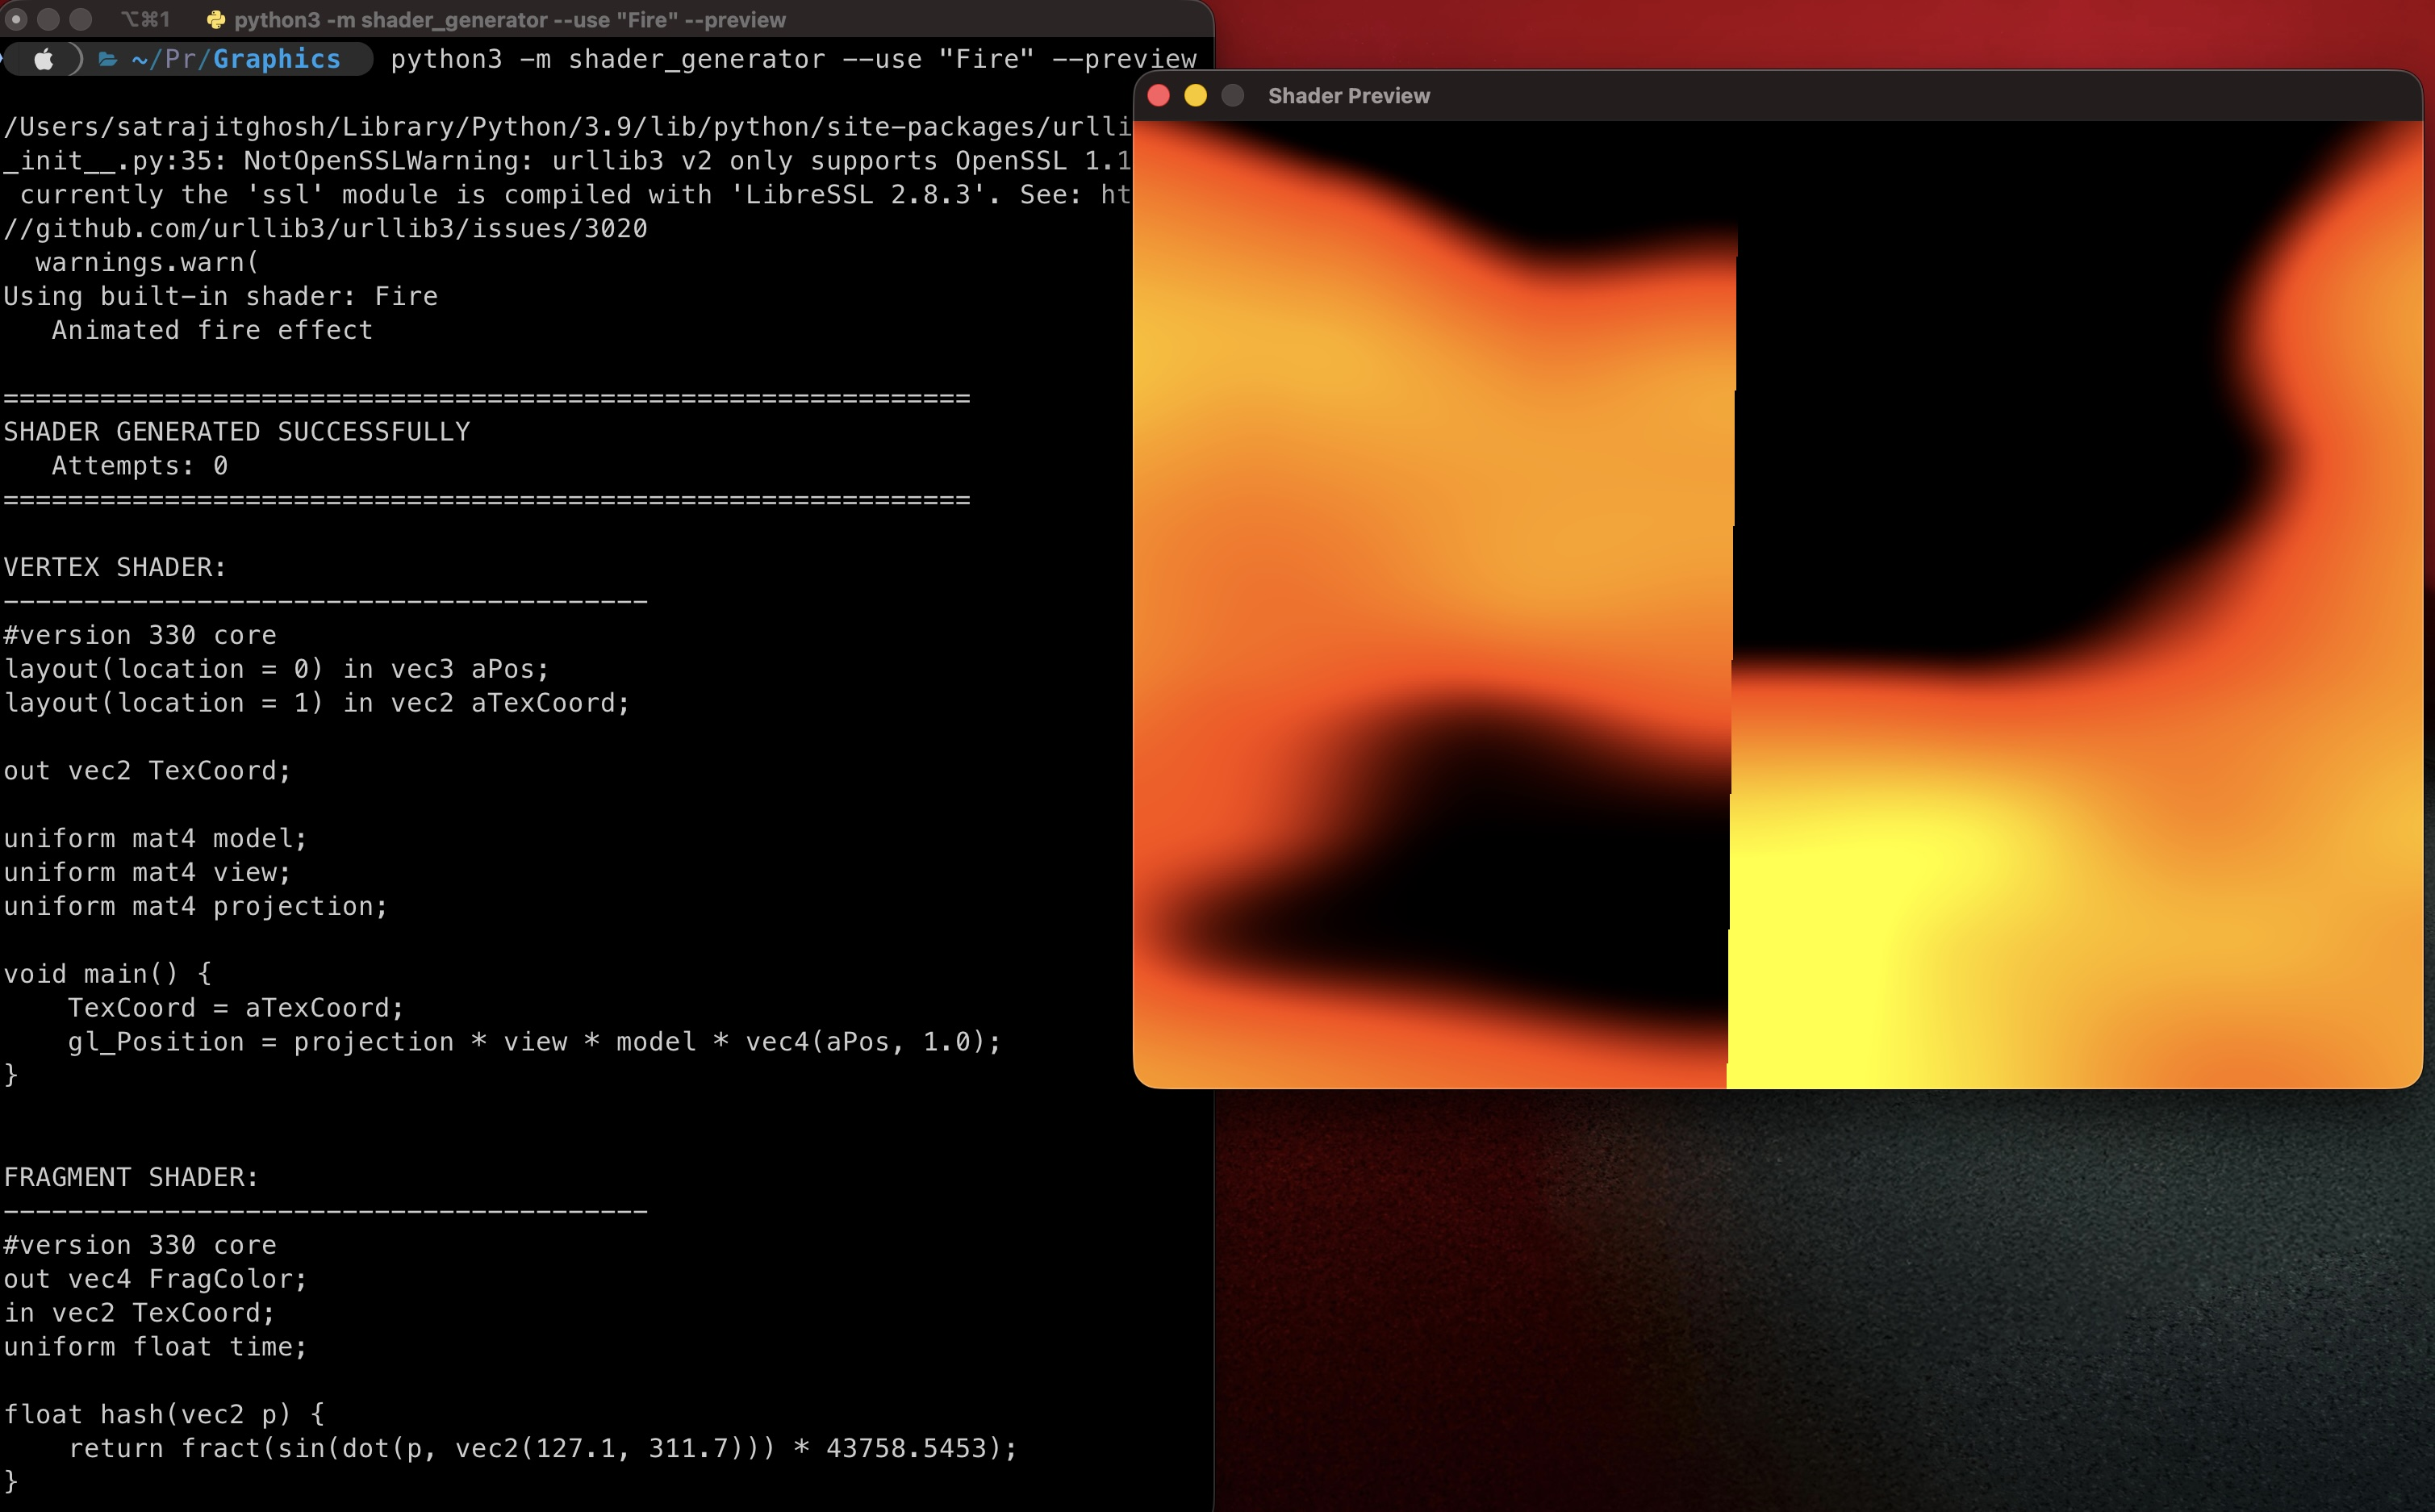
\includegraphics[width=\textwidth]{images/ShaderGenerator.jpg.jpeg}
    \caption{Generated Mandelbrot GLSL source and animated preview.}
    \label{fig:shader_mandelbrot_code}
  \end{subfigure}\hfill
  \begin{subfigure}[t]{0.48\textwidth}
    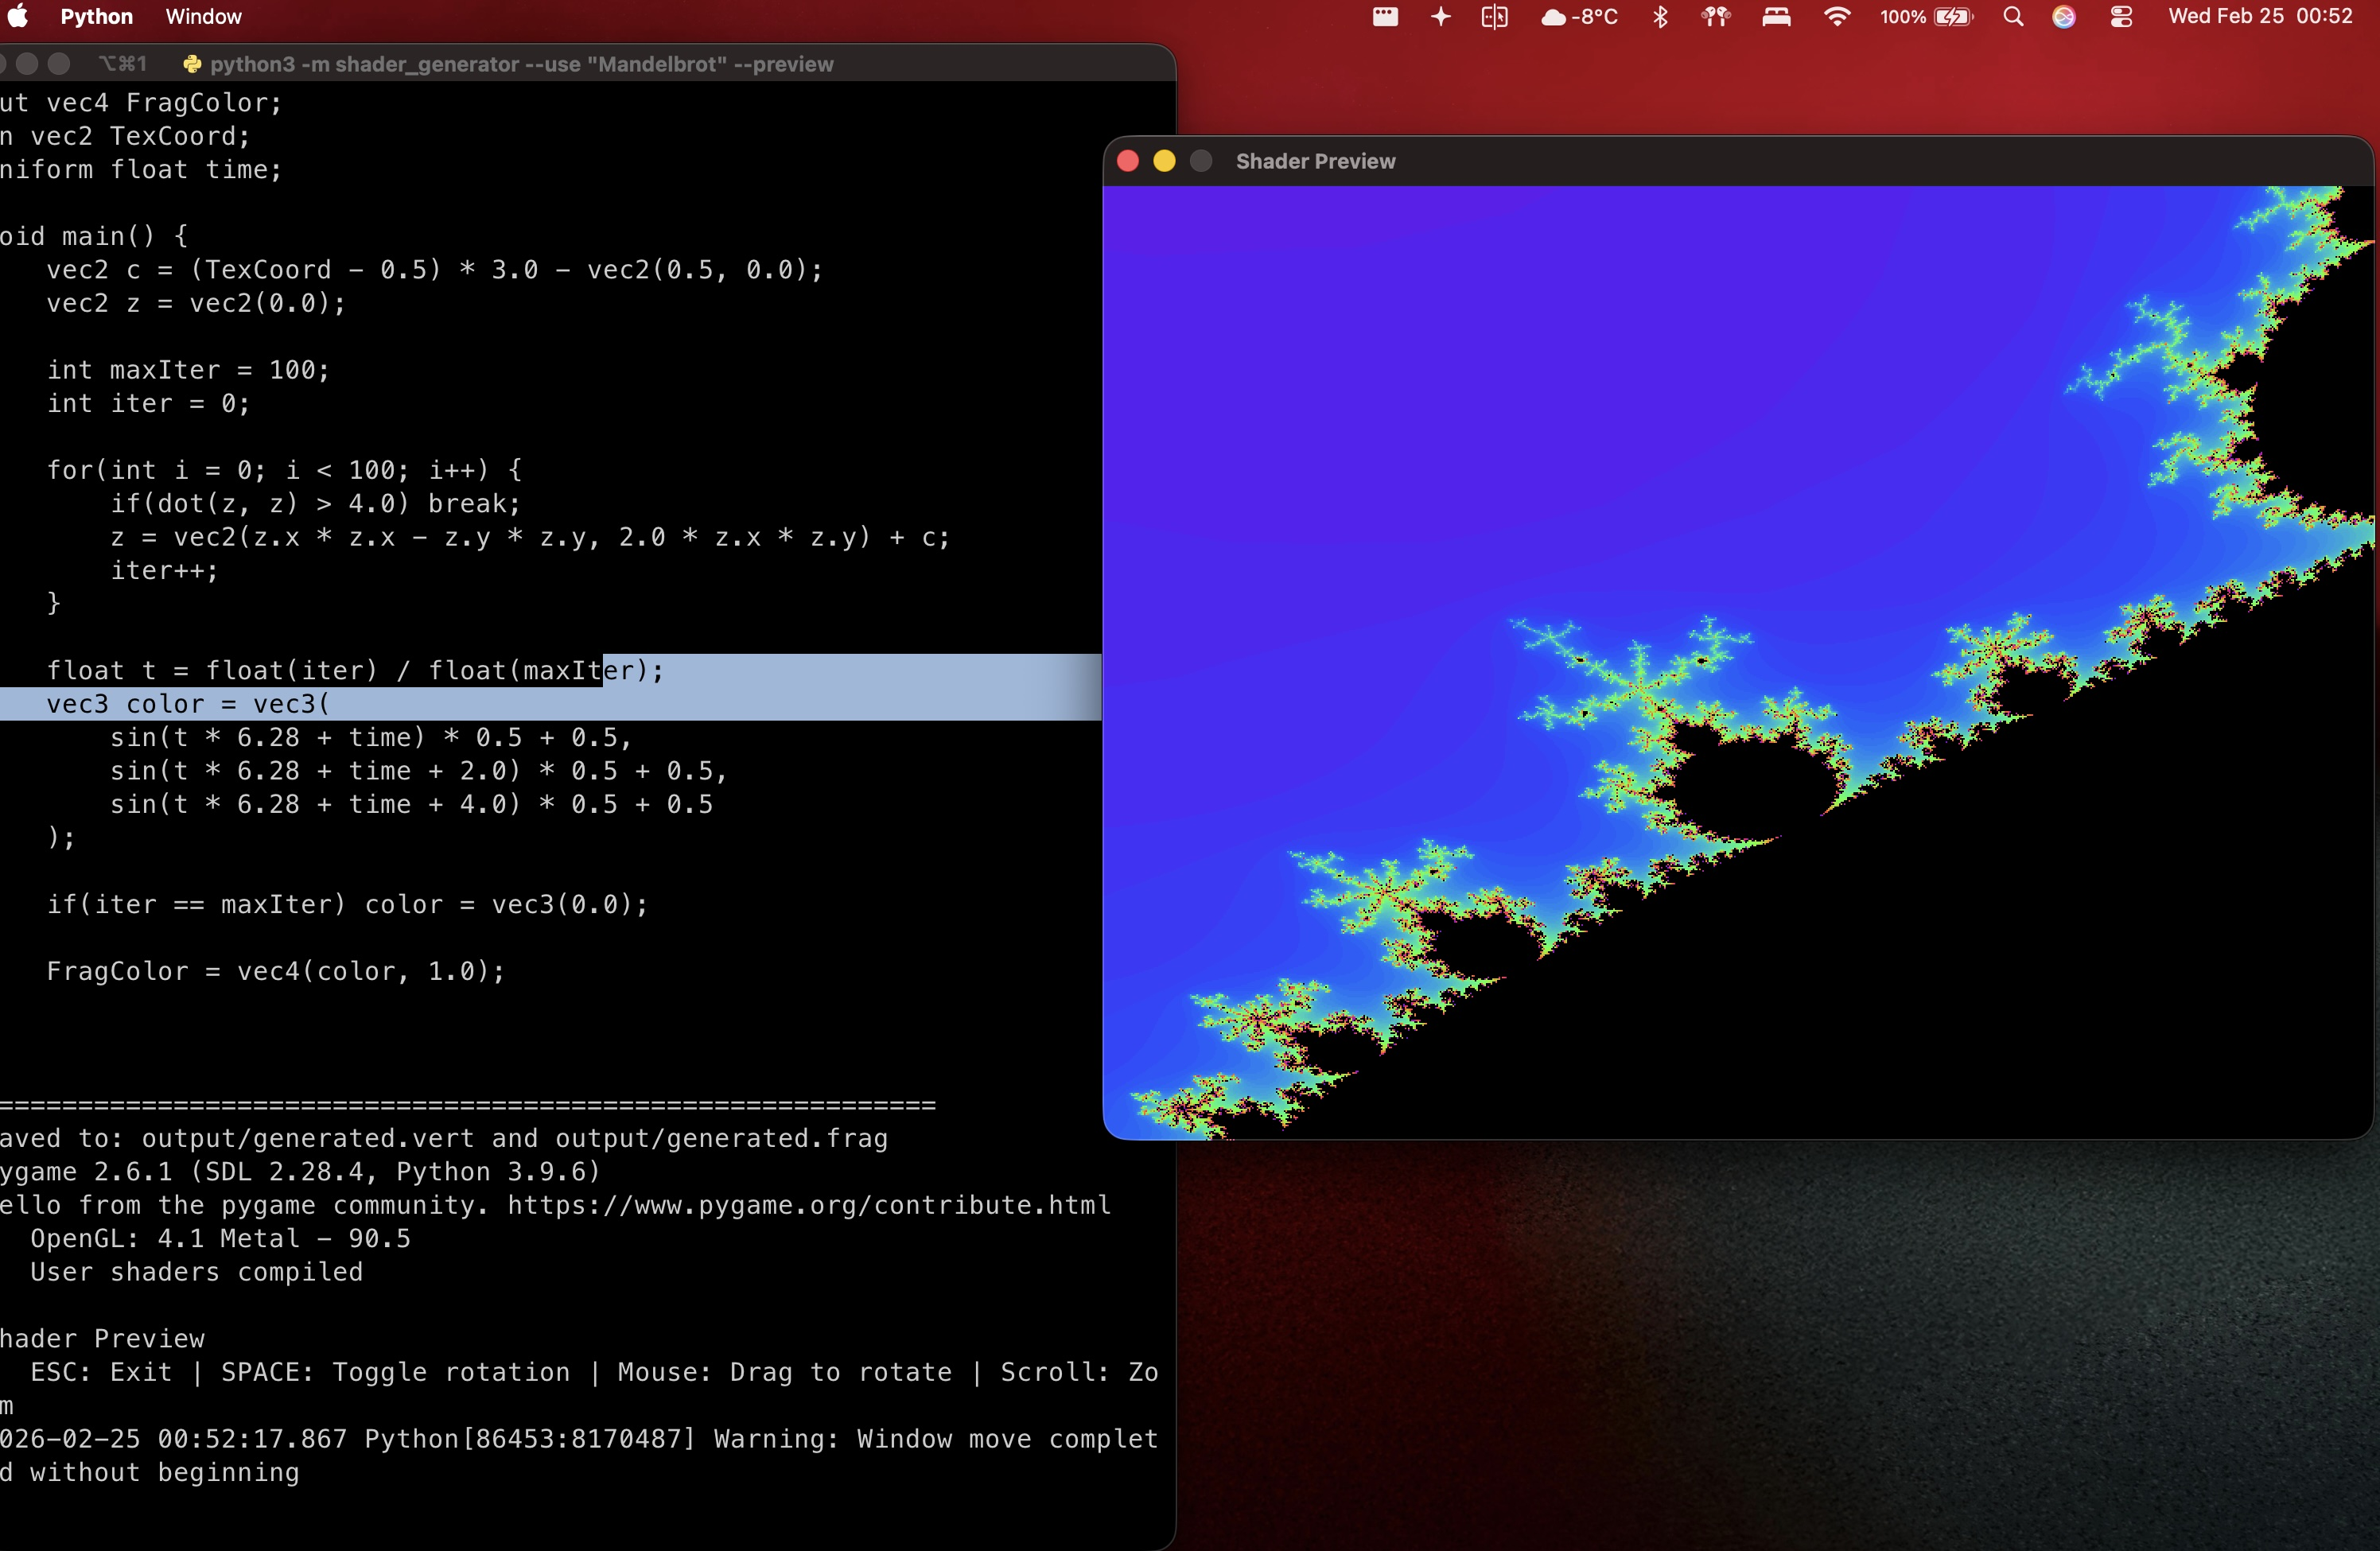
\includegraphics[width=\textwidth]{images/ShaderGenerator2.jpg.jpeg}
    \caption{Mandelbrot set rendered at full resolution.}
    \label{fig:shader_mandelbrot_preview}
  \end{subfigure}
  \caption{Natural language shader generation: Mandelbrot and fire prompt producing
           a compilable animated GLSL shader on the first attempt.These show the noise-based animated fragment shader source alongside the live preview}
  \label{fig:shader_mandelbrot}
\end{figure}

\begin{figure}[H]
  \centering
  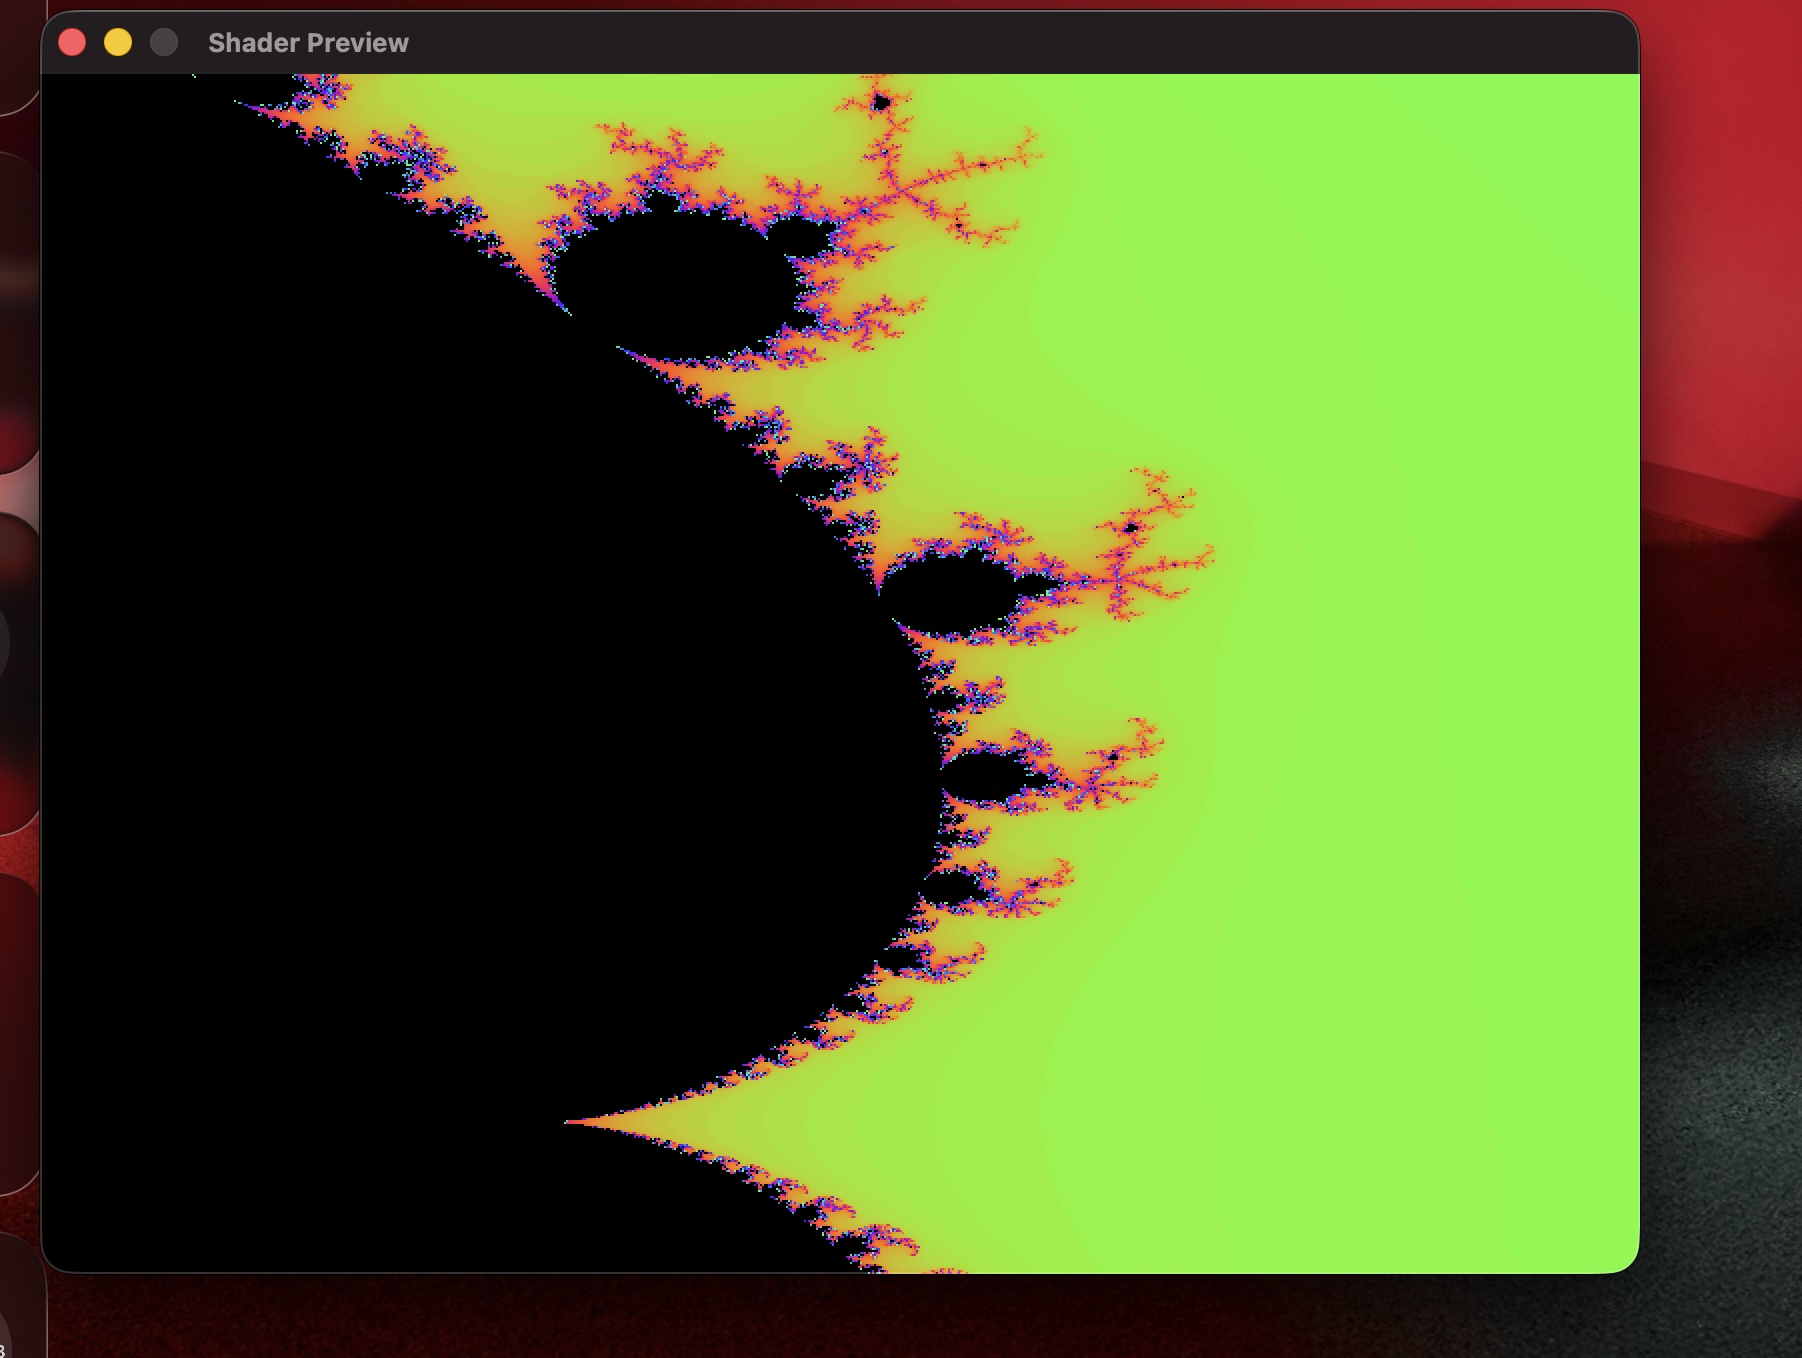
\includegraphics[width=0.85\textwidth]{images/ShaderGenerator3.jpg.jpeg}
  \caption{Mandelbrot with green background shader generated from the prompt \texttt{"Mandelbrot with neon green background"}, showing
           the live preview. Zero compilation repair attempts were required.}
  \label{fig:shader_fire}
\end{figure}




\subsection{LLM-Assisted CMake Generation}

The CMake generator was evaluated using the SPH fluid demonstration project
as a test case. The tool uses Qwen2.5-Coder 7B
(\texttt{qwen2.5:7b-instruct-q4\_K\_M}) running locally through Ollama at
temperature 0.3~\cite{hui2024qwen25coder,ollama2024}.

Figure~\ref{fig:cmake_step1} shows the first two steps of the pipeline. In
Step~1, the tool analyses the project directory structure, detecting four
source files (\texttt{main.cpp}, \texttt{sph.cpp}, \texttt{renderer.cpp},
\texttt{gui.cpp}), four headers, an SFML dependency, C++17 as the language
standard, and an executable target type. In Step~2, this information is
injected into a structured system prompt that instructs the model to output
only valid \texttt{CMakeLists.txt} content with no explanations or markdown,
using modern CMake practices including target-based commands, generator
expressions, and \texttt{find\_package} for external dependencies. The total
prompt length was 1{,}340 characters.

Figure~\ref{fig:cmake_step3} shows Step~3, where the model streams the
generated \texttt{CMakeLists.txt} in real time, followed by Step~4 displaying
the final 26-line output saved to disk. The generated file correctly set up
the project, configured C++17, listed all source files, linked SFML, and
included install rules.

\begin{figure}[H]
  \centering
  \begin{subfigure}[t]{0.48\textwidth}
    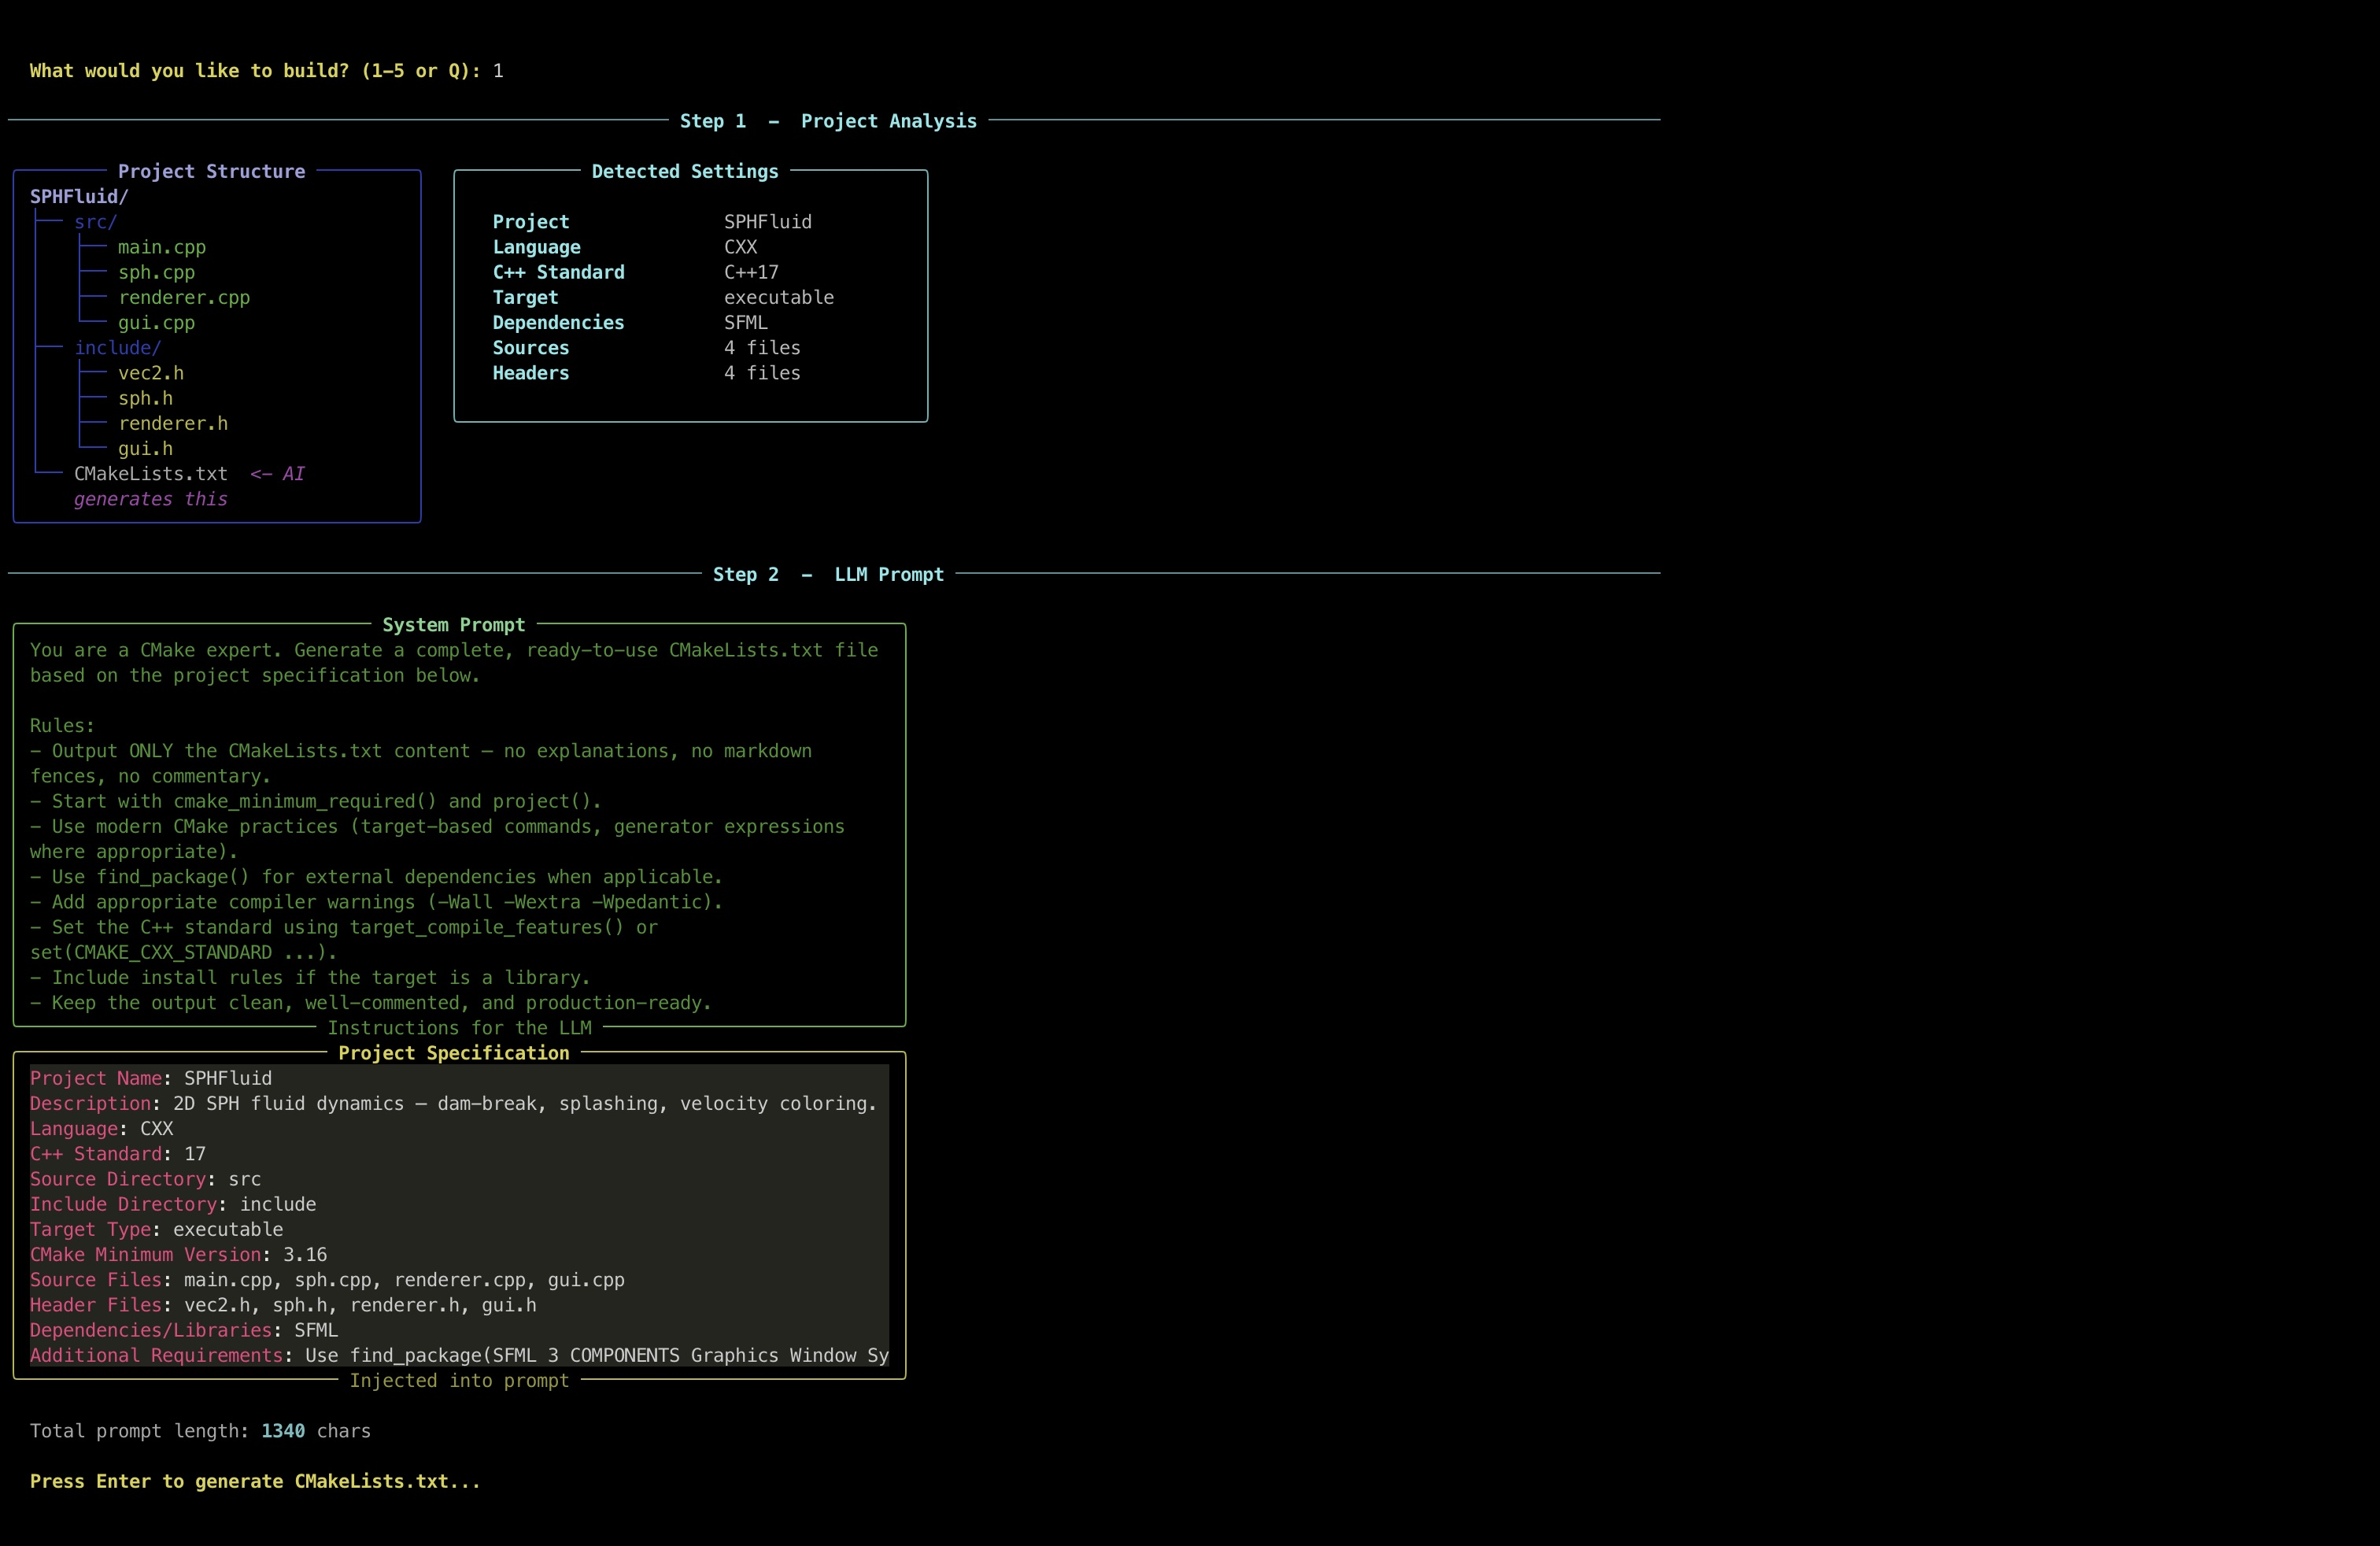
\includegraphics[width=\textwidth]{images/CmakeGenerator1.jpg}
    \caption{Step 1: project analysis and Step 2: structured LLM prompt with
             injected project specification.}
    \label{fig:cmake_step1}
  \end{subfigure}\hfill
  \begin{subfigure}[t]{0.48\textwidth}
    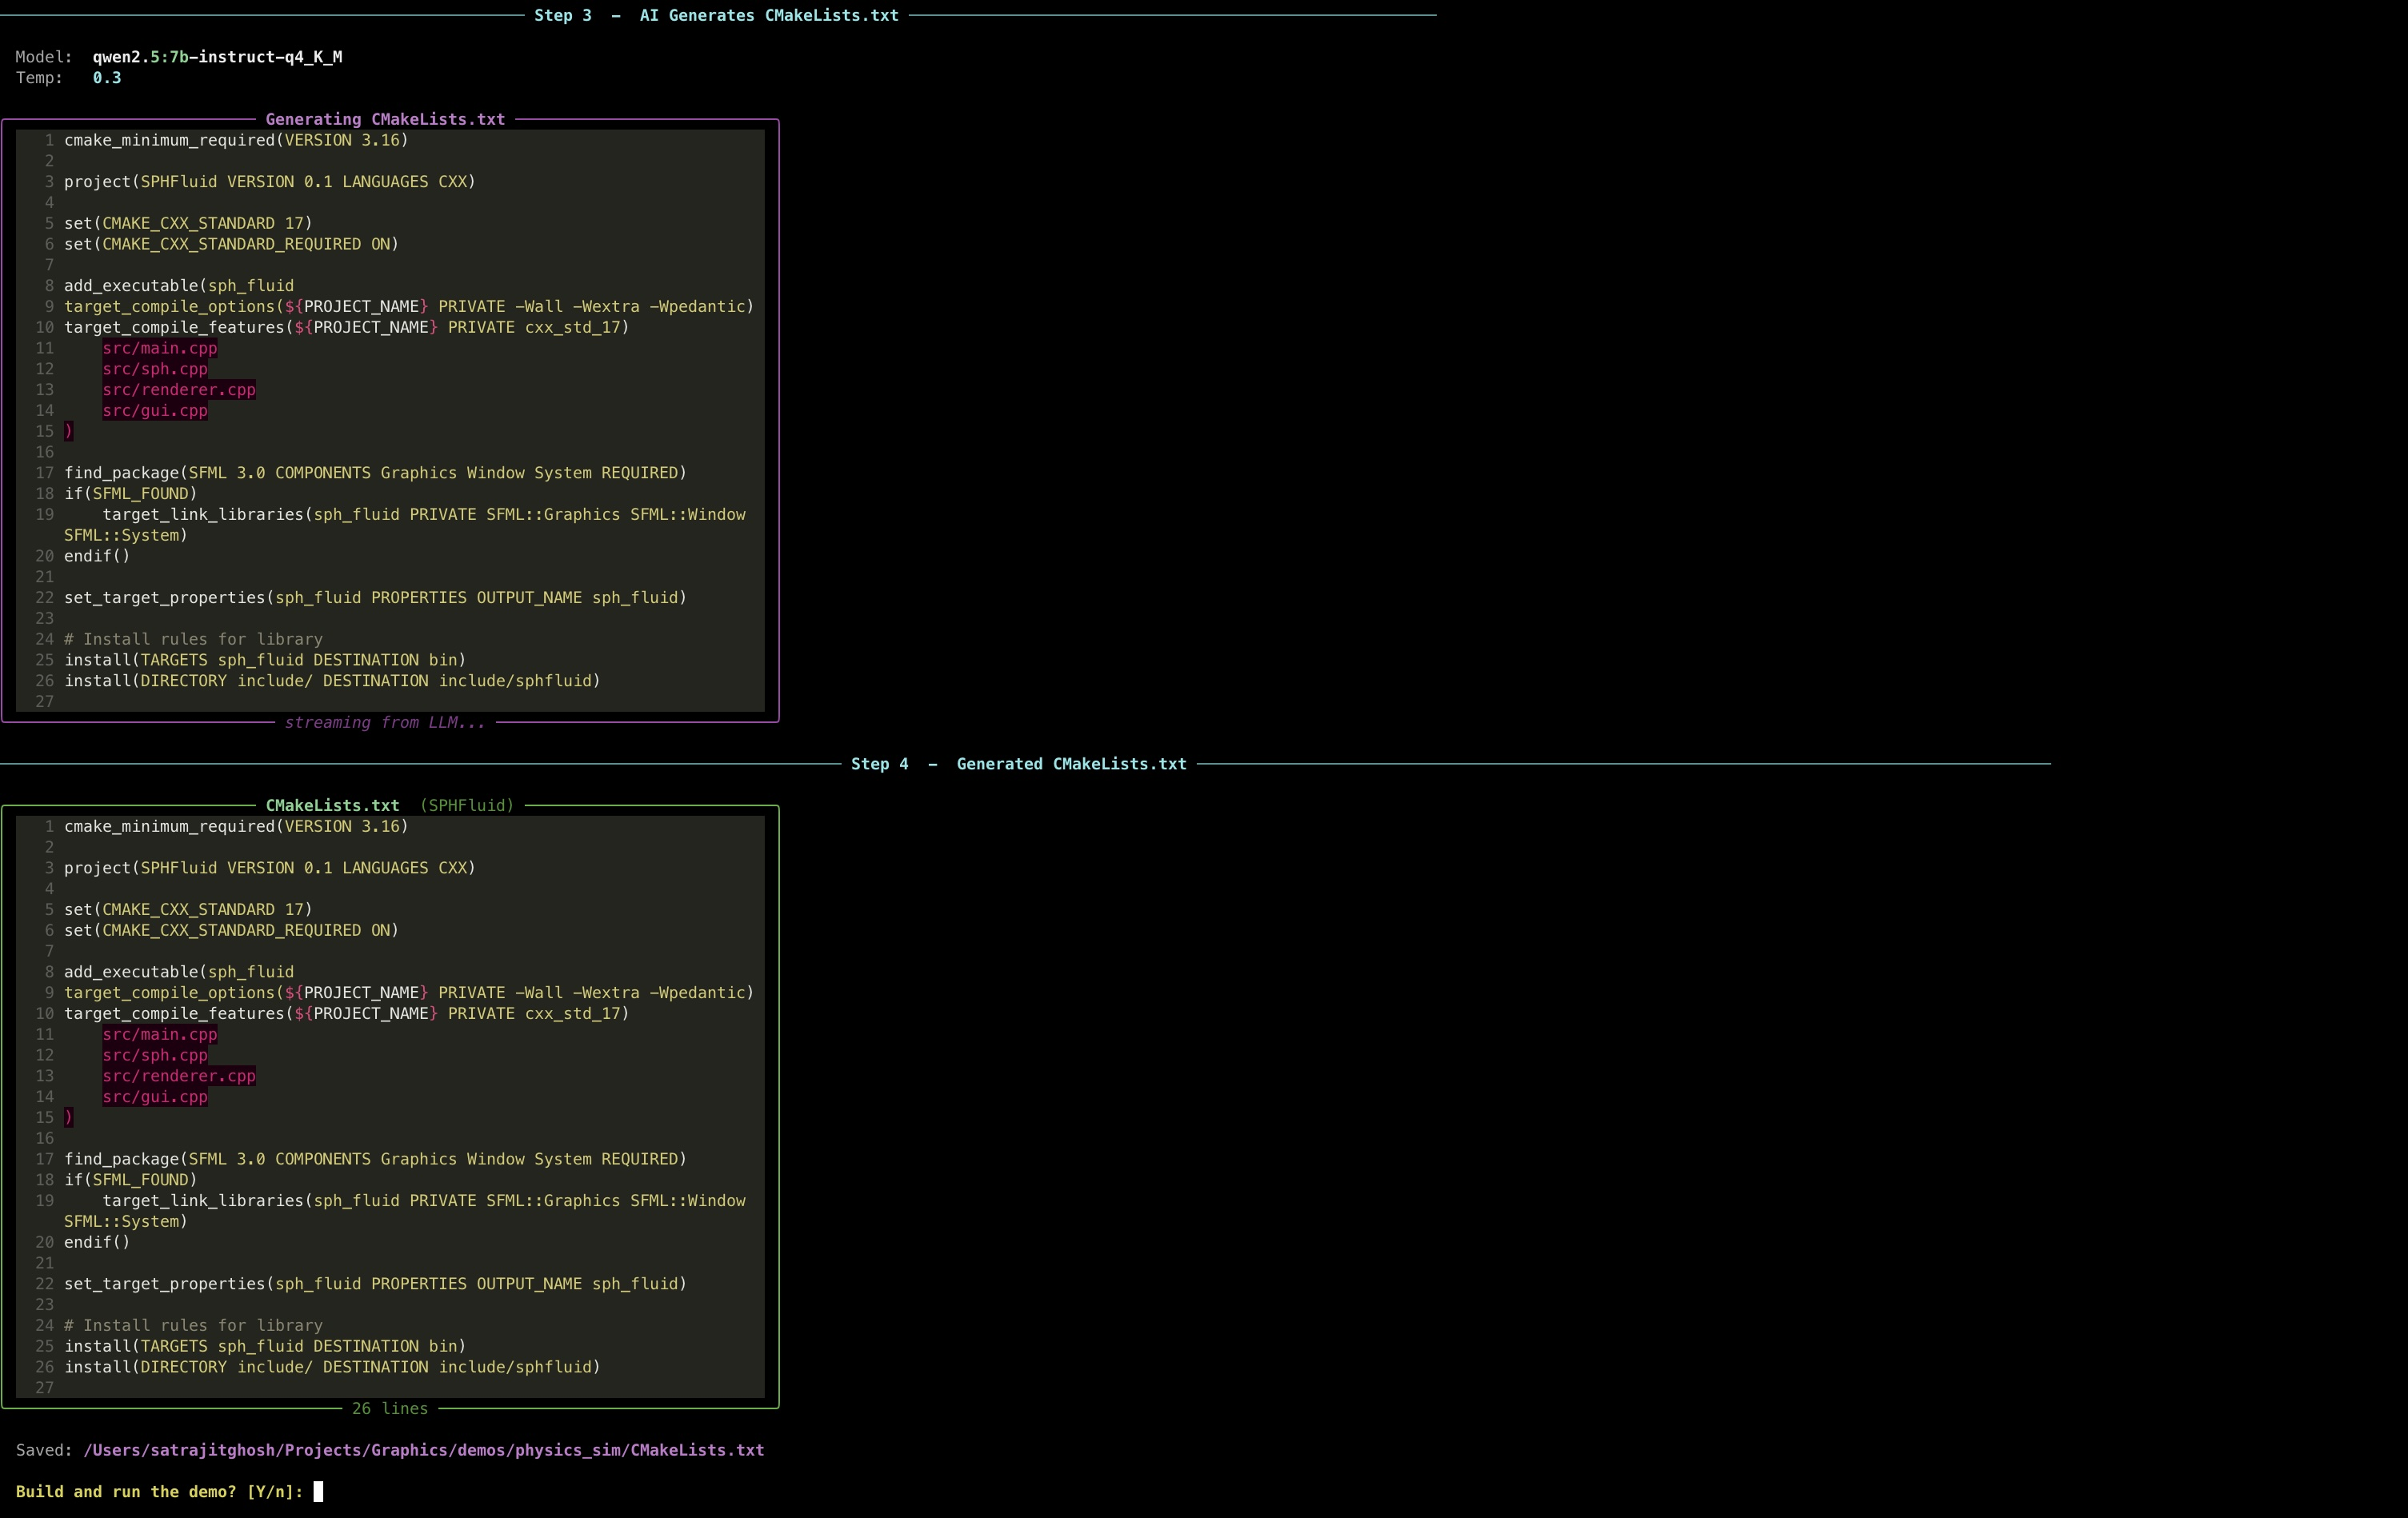
\includegraphics[width=\textwidth]{images/Cmake Generator2.jpg}
    \caption{Step 3: Qwen2.5-Coder 7B streaming CMakeLists.txt generation
             and Step 4: final saved output.}
    \label{fig:cmake_step3}
  \end{subfigure}
  \caption{CMake generation pipeline: project analysis, prompt construction,
           and LLM-driven output using locally hosted Qwen2.5-Coder 7B.}
  \label{fig:cmake_gen}
\end{figure}

The initial build attempt failed with a CMake error at
\texttt{add\_executable} (Figure~\ref{fig:cmake_fail}). The tool detected the
failure and offered to send the error back to the model for automatic repair.
Figure~\ref{fig:cmake_fix} shows the auto-fix loop: the error message was
forwarded to the LLM, which produced a corrected \texttt{CMakeLists.txt}
adding the missing \texttt{target\_include\_directories} directive and
properly closing the \texttt{add\_executable} block. The fixed file grew from
26 to 30 lines.

After the repair, the build succeeded on the second attempt, compiling across
12 threads, and the SPH fluid demo launched directly from the terminal
(Figure~\ref{fig:cmake_success}). The full cycle from project analysis
through generation, failed build, automatic repair, successful build, and
demo launch completed without any manual editing of the
\texttt{CMakeLists.txt} file.

\begin{figure}[H]
  \centering
  \begin{subfigure}[t]{0.48\textwidth}
    
\includegraphics[width=\textwidth]{images/Cmake3.jpg}
    \caption{Step 5: initial build fails; tool offers AI-driven repair.}
    \label{fig:cmake_fail}
  \end{subfigure}\hfill
  \begin{subfigure}[t]{0.48\textwidth}
    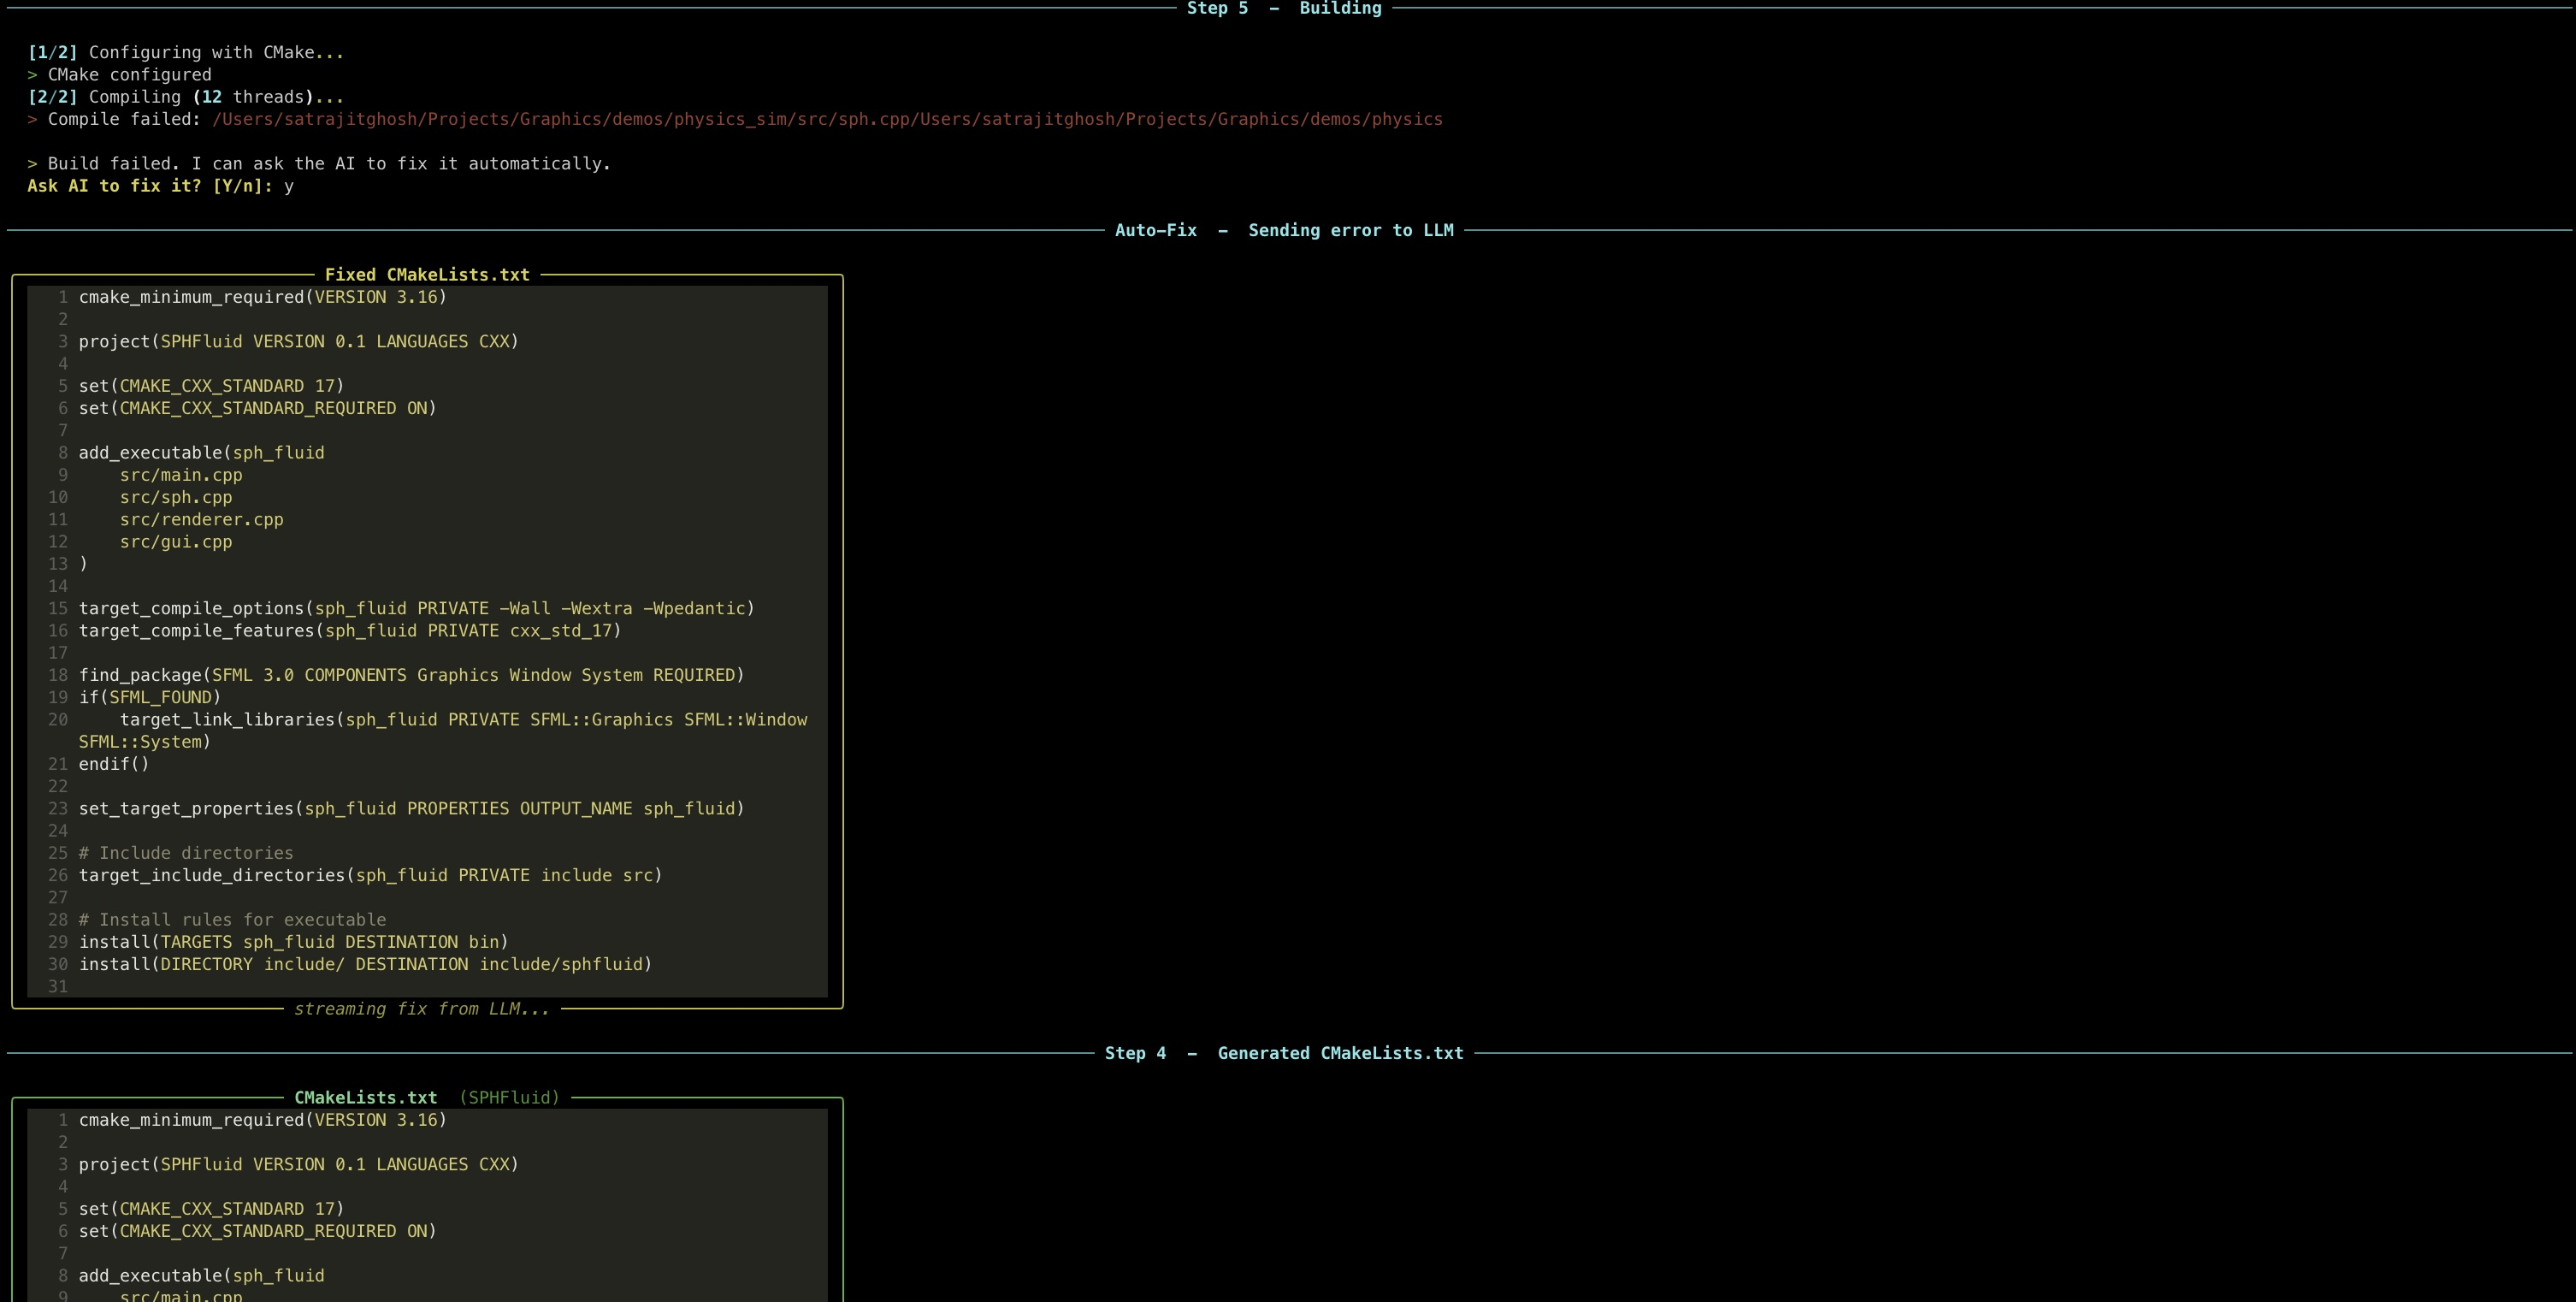
\includegraphics[width=\textwidth]{images/Cmake4.jpg}
    \caption{Auto-fix: error sent to LLM, corrected CMakeLists.txt
             generated with include directory fix.}
    \label{fig:cmake_fix}
  \end{subfigure}
  \caption{Build failure and automatic LLM-driven repair loop.}
  \label{fig:cmake_repair}
\end{figure}

\begin{figure}[H]
  \centering
  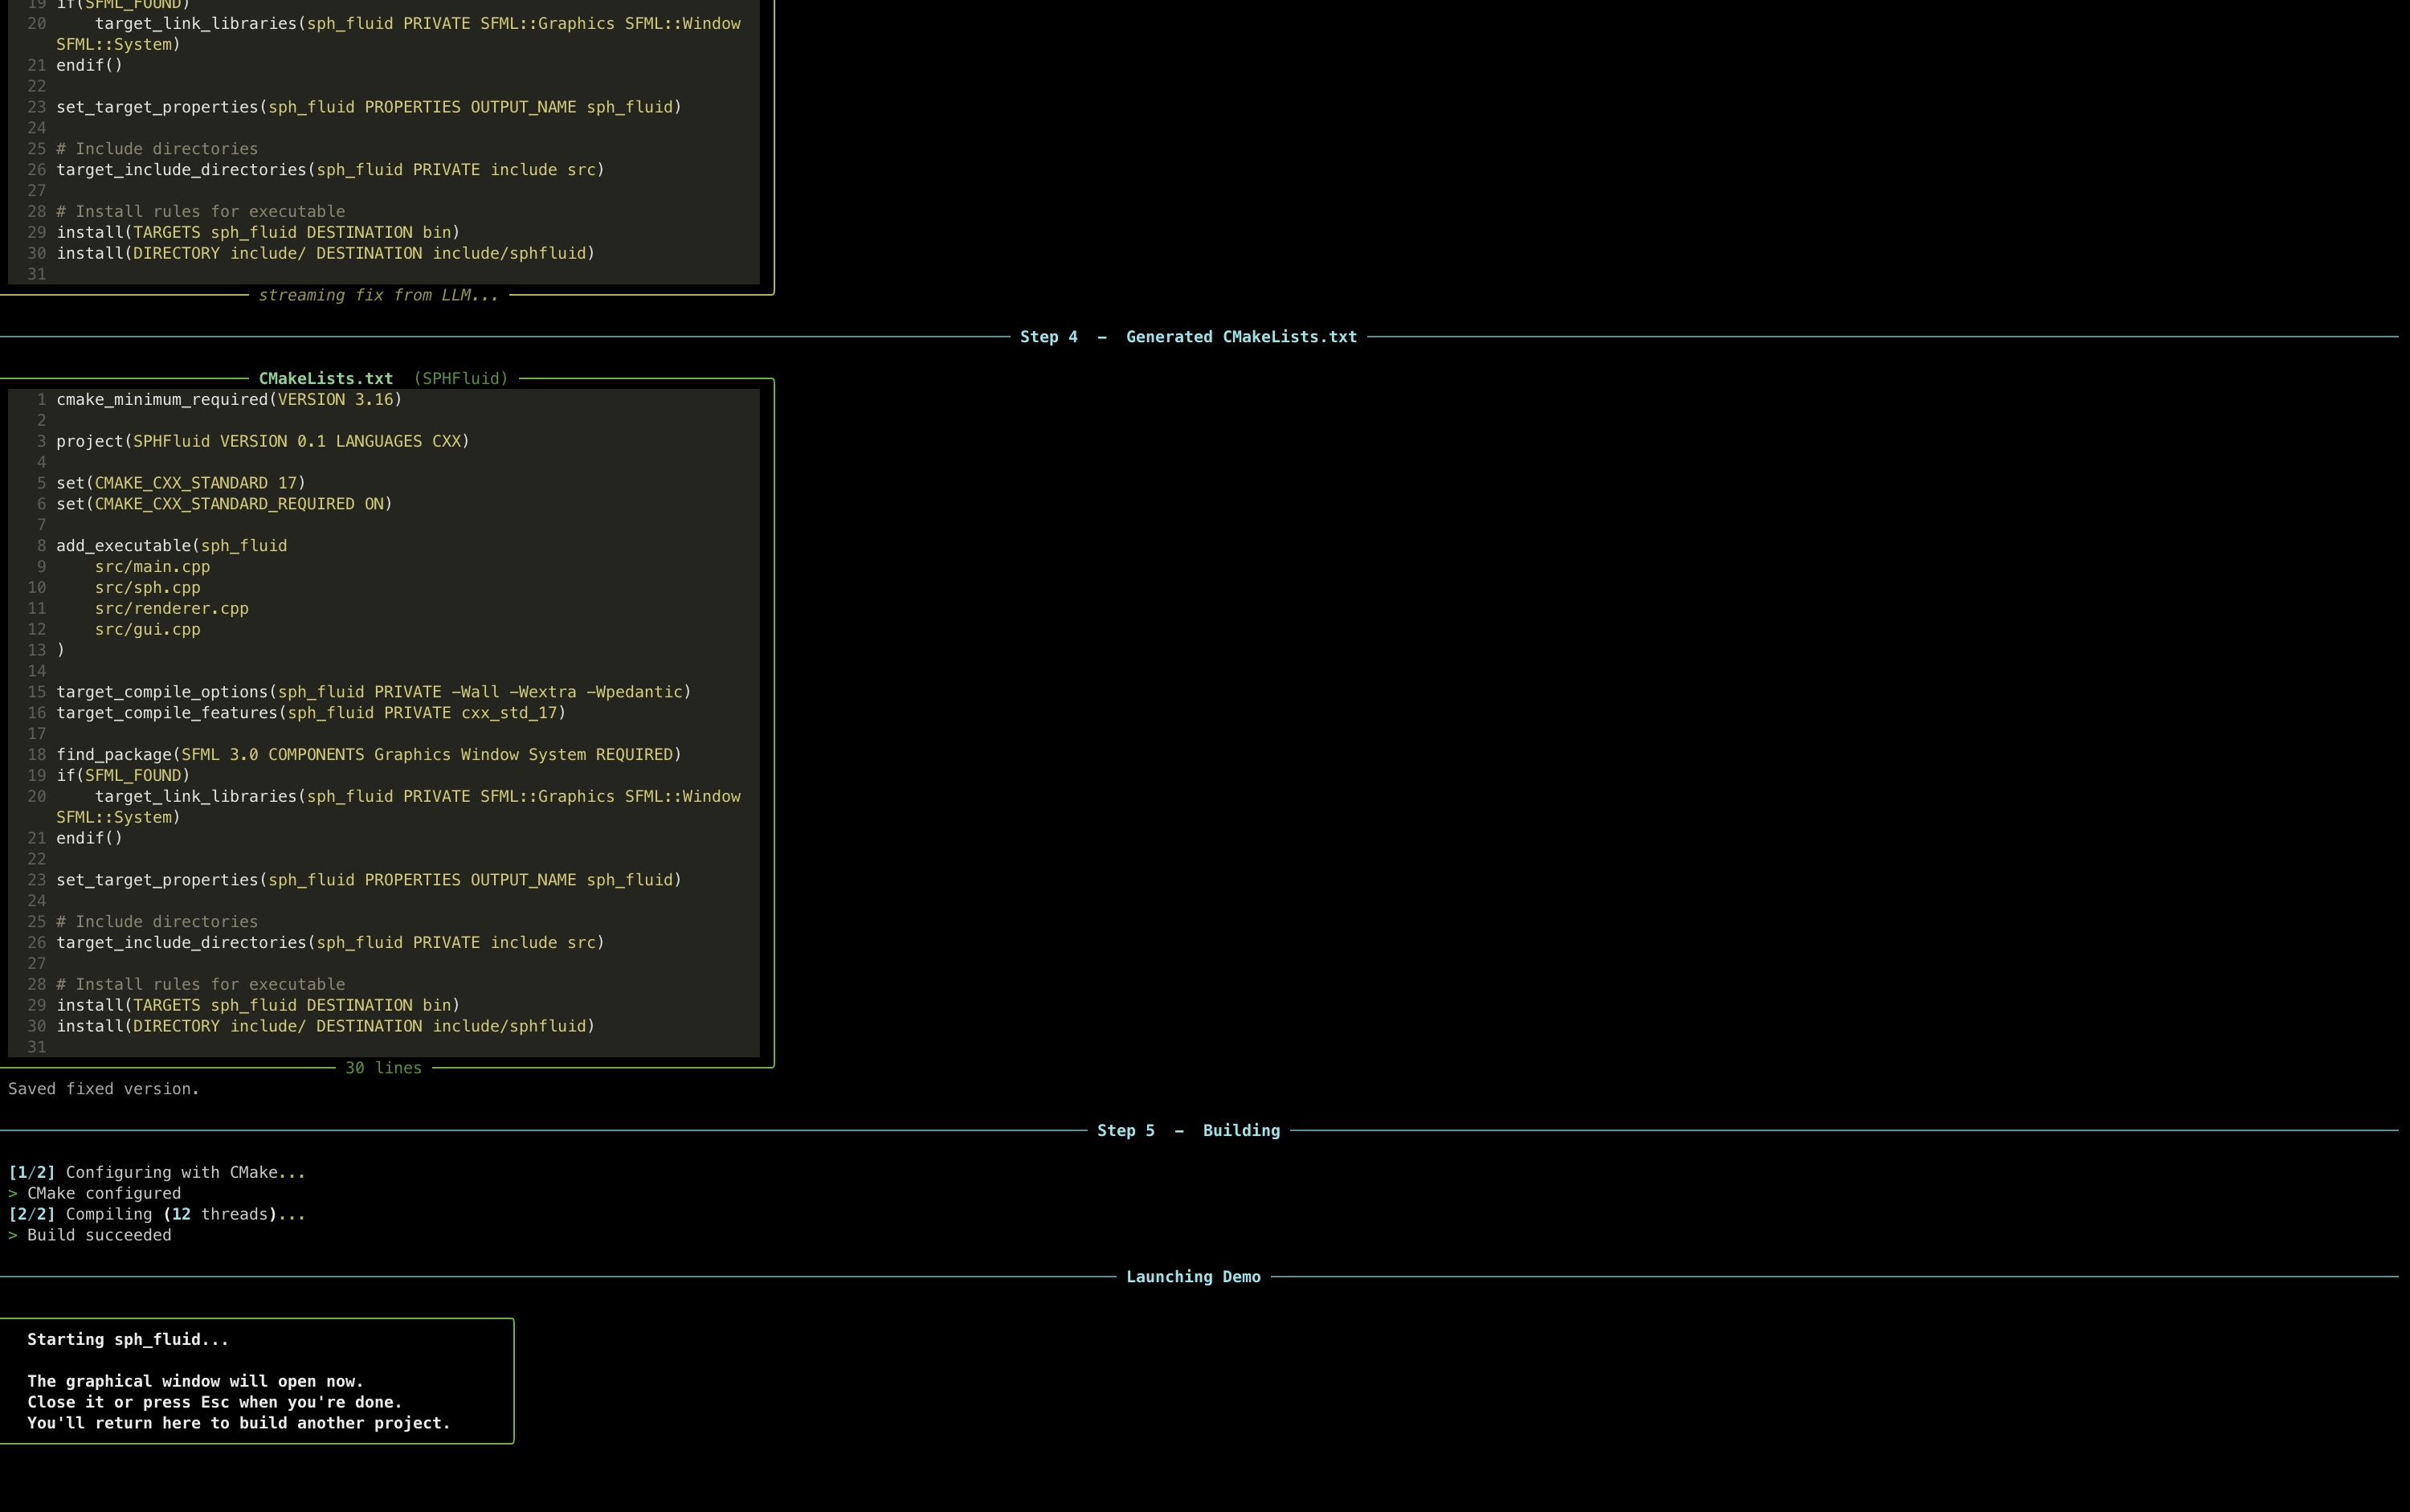
\includegraphics[width=0.85\textwidth]{images/Cmake6.jpg}
  \caption{Successful build after automatic repair, compiling with 12 threads
           and launching the SPH fluid demo directly from the terminal.}
  \label{fig:cmake_success}
\end{figure}
% ═══════════════════════════════════════════════════════════════════════════
\section{RL Auto-Tuner Results}
% ═══════════════════════════════════════════════════════════════════════════

\subsection{Parallelism Baseline}

Before evaluating the RL agent, the impact of the job system was established.
Figure~\ref{fig:rl_slow} shows single-threaded execution with 8{,}000 bodies,
producing a frame time of 366.72~ms (3~FPS) with gravity and collision each
contributing over 100~ms due to their $O(n^2)$ complexity.
Figure~\ref{fig:rl_fast} shows the parallel configuration with 2{,}500 bodies
across 11 workers, reducing total physics time to 12.6~ms (50~FPS).
Per-worker utilisation ranged from 19\% to 49\%, indicating workload
imbalance that the job scheduler environment was designed to address.

\begin{figure}[H]
  \centering
  \begin{subfigure}[t]{0.48\textwidth}
    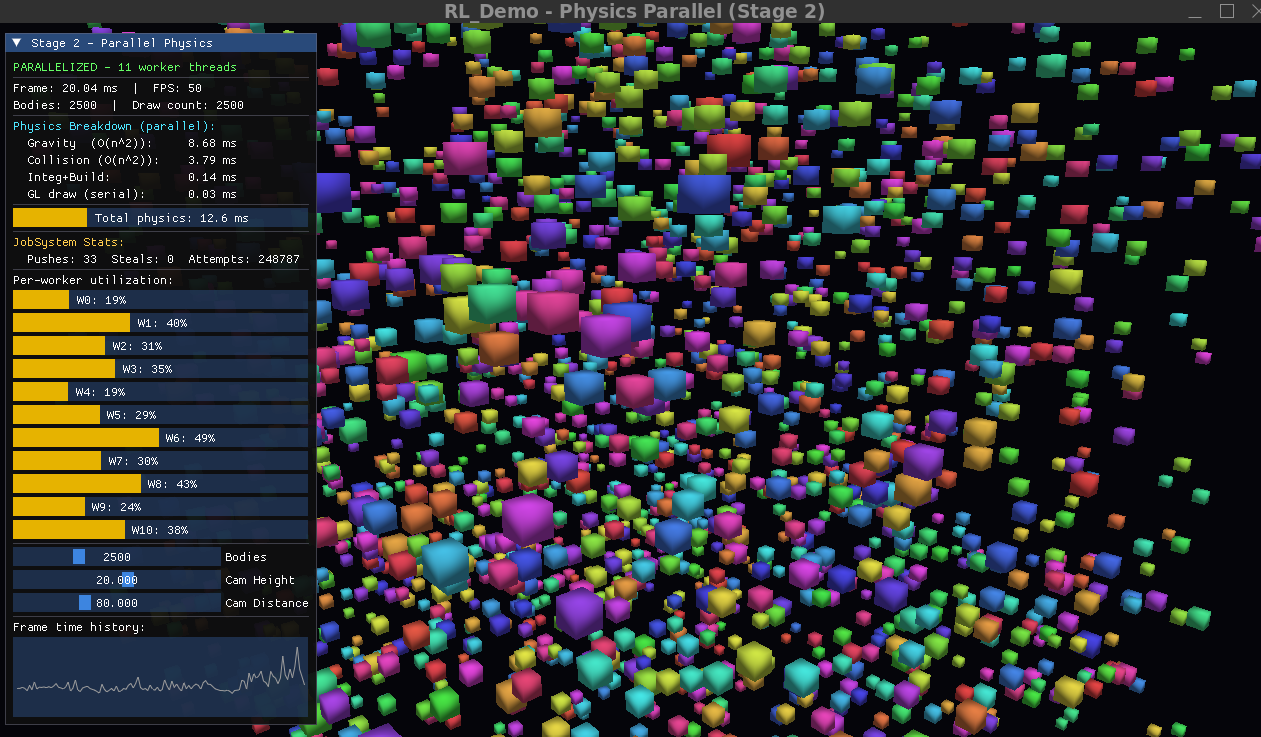
\includegraphics[width=\textwidth]{images/RL Env Demo.png}
    \caption{Single-threaded: 8{,}000 bodies, 366.72~ms, 3~FPS.}
    \label{fig:rl_slow}
  \end{subfigure}\hfill
  \begin{subfigure}[t]{0.48\textwidth}
    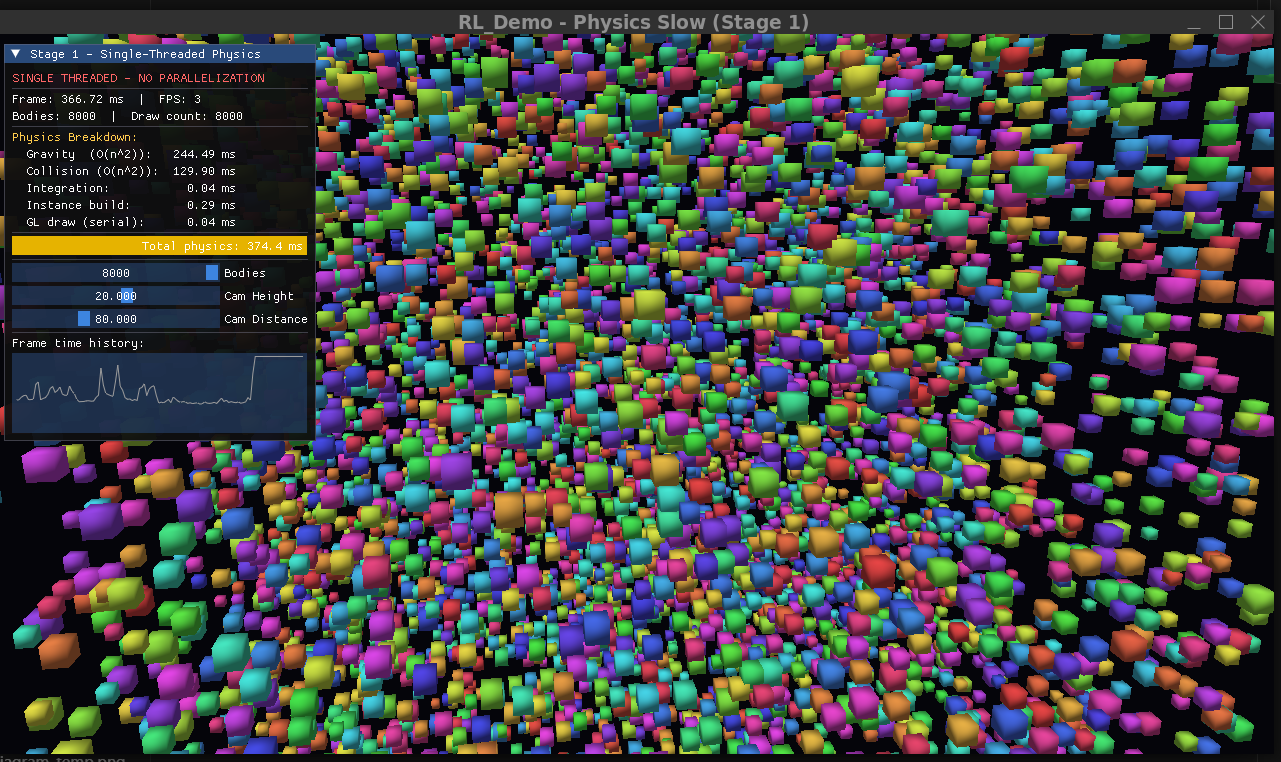
\includegraphics[width=\textwidth]{images/RL Env Demo 2.png}
    \caption{Parallelised: 8{,}000 bodies, 20.04~ms, 50~FPS.}
    \label{fig:rl_fast}
  \end{subfigure}
  \caption{Single-threaded versus 11-worker parallel physics execution showing
           the workload imbalance visible in per-worker utilisation bars.}
  \label{fig:rl_parallel}
\end{figure}

\subsection{Frame Scheduler Environment}

Table~\ref{tab:frame_scheduler} presents RL agent results against fixed-count
baselines for the \texttt{FrameSchedulerEnv}.  The PPO agent achieved an
average frame time of 9.070~ms, a 23.79\% improvement over the best static
baseline (10k cubes, 11.901~ms).  The agent also reduced the p95 latency from
18.687~ms to 15.269~ms, demonstrating that dynamic scene parameter adjustment
produces lower and more consistent frame times than any fixed configuration.

\begin{table}[H]
  \centering
  \caption{FrameSchedulerEnv: PPO agent versus fixed-count baselines
           (100 benchmark steps).}
  \label{tab:frame_scheduler}
  \begin{tabular}{lrrrr}
    \toprule
    Configuration & Avg (ms) & Min (ms) & Max (ms) & p95 (ms) \\
    \midrule
    1k cubes    & 12.389 & 7.754  & 45.942 & 18.687 \\
    10k cubes   & 11.901 & 8.593  & 22.010 & 15.248 \\
    50k cubes   & 15.648 & 12.774 & 24.233 & 18.761 \\
    100k cubes  & 20.248 & 15.419 & 31.320 & 24.838 \\
    \midrule
    \textbf{PPO agent} & \textbf{9.070} & \textbf{5.404} & 29.661 & \textbf{15.269} \\
    \bottomrule
  \end{tabular}
\end{table}

\subsection{Job Scheduler Environment}

Four experiments evaluated the \texttt{JobSchedulerEnv} across varying body
counts and workload distributions.  Results are summarised in
Table~\ref{tab:job_scheduler_summary} and detailed in
Tables~\ref{tab:job_nonuniform}--\ref{tab:job_alternate}.

\begin{table}[H]
  \centering
  \caption{JobSchedulerEnv summary: PPO agent versus best baseline
           per scenario.}
  \label{tab:job_scheduler_summary}
  \begin{tabular}{llrrr}
    \toprule
    Scenario & Best Baseline & Baseline (ms) & RL (ms) & Change \\
    \midrule
    Non-uniform 100k  & linear\_decrease & 9.620  & 8.634  & \textbf{+10.24\%} \\
    Uniform 100k      & uniform          & 7.921  & 8.313  & $-$4.96\%  \\
    High load 200k    & uniform          & 9.515  & 10.561 & $-$10.99\% \\
    Alternate 100k    & complexity\_aware & 8.376 & 9.931  & $-$18.58\% \\
    \bottomrule
  \end{tabular}
\end{table}

\begin{table}[H]
  \centering
  \caption{Experiment 2A: Non-uniform workload, 100k cubes, 150 steps.}
  \label{tab:job_nonuniform}
  \begin{tabular}{lrrr}
    \toprule
    Strategy          & Avg (ms) & Std (ms) & p95 (ms) \\
    \midrule
    uniform           & 10.680 & 2.800  & 17.989 \\
    front\_heavy      & 11.198 & 1.749  & 14.661 \\
    back\_heavy       & 19.015 & 102.944 & 14.806 \\
    alternating       & 10.132 & 2.875  & 12.794 \\
    single\_heavy     & 9.725  & 2.149  & 14.501 \\
    complexity\_aware & 10.014 & 1.494  & 12.515 \\
    linear\_decrease  & 9.620  & 1.565  & 12.461 \\
    \midrule
    \textbf{PPO agent} & \textbf{8.634} & \textbf{0.802} & \textbf{10.001} \\
    \bottomrule
  \end{tabular}
\end{table}

\begin{table}[H]
  \centering
  \caption{Experiment 2B: Uniform workload, 100k cubes, 200 steps.}
  \label{tab:job_uniform}
  \begin{tabular}{lrrr}
    \toprule
    Strategy          & Avg (ms) & Std (ms) & p95 (ms) \\
    \midrule
    uniform           & \textbf{7.921} & 0.505 & \textbf{9.001} \\
    front\_heavy      & 8.722 & 2.401 & 11.579 \\
    back\_heavy       & 8.470 & 0.943 & 10.283 \\
    alternating       & 8.873 & 1.967 & 11.611 \\
    single\_heavy     & 8.827 & 1.668 & 11.801 \\
    complexity\_aware & 8.467 & 1.918 & 10.652 \\
    linear\_decrease  & 9.559 & 2.274 & 14.081 \\
    \midrule
    PPO agent         & 8.313 & 1.171 & 9.755 \\
    \bottomrule
  \end{tabular}
\end{table}

\begin{table}[H]
  \centering
  \caption{Experiment 2C: High load, 200k cubes, 150 steps.}
  \label{tab:job_highload}
  \begin{tabular}{lrrr}
    \toprule
    Strategy      & Avg (ms) & Std (ms) & p95 (ms) \\
    \midrule
    uniform       & \textbf{9.515}  & 1.053  & \textbf{11.763} \\
    front\_heavy  & 10.114 & 1.530  & 13.145 \\
    back\_heavy   & 10.005 & 0.959  & 11.633 \\
    alternating   & 10.482 & 1.182  & 12.686 \\
    single\_heavy & 14.715 & 10.560 & 42.390 \\
    \midrule
    PPO agent     & 10.561 & 1.128  & 12.549 \\
    \bottomrule
  \end{tabular}
\end{table}

\begin{table}[H]
  \centering
  \caption{Experiment 2D: Alternate run, 100k cubes, 150 steps.}
  \label{tab:job_alternate}
  \begin{tabular}{lrrr}
    \toprule
    Strategy          & Avg (ms) & Std (ms) & p95 (ms) \\
    \midrule
    uniform           & 19.271 & 6.840 & 31.634 \\
    front\_heavy      & 17.620 & 3.643 & 24.112 \\
    back\_heavy       & 13.492 & 5.215 & 22.439 \\
    alternating       & 10.616 & 3.019 & 16.434 \\
    single\_heavy     & 9.214  & 1.736 & 11.811 \\
    complexity\_aware & \textbf{8.376}  & 1.624 & \textbf{10.855} \\
    linear\_decrease  & 8.629  & 0.935 & 10.668 \\
    \midrule
    PPO agent         & 9.931  & 2.137 & 14.914 \\
    \bottomrule
  \end{tabular}
\end{table}

% TikZ bar chart: RL vs best baseline per scenario
\begin{figure}[H]
\centering
\begin{tikzpicture}
\begin{axis}[
    ybar,
    bar width=14pt,
    width=0.85\textwidth,
    height=6.5cm,
    legend style={at={(0.97,0.97)}, anchor=north east, font=\small},
    symbolic x coords={FrameSched, Job-NonUniform, Job-Uniform, Job-HighLoad},
    xtick=data,
    xticklabel style={font=\small},
    ymin=0, ymax=14,
    ylabel={Average frame time (ms)},
    ylabel style={font=\small},
    nodes near coords,
    nodes near coords style={font=\tiny},
    every axis plot/.append style={line width=0pt},
]
\addplot[fill=blueBox!80, draw=none]
    coordinates {
        (FrameSched,11.901)
        (Job-NonUniform,9.620)
        (Job-Uniform,7.921)
        (Job-HighLoad,9.515)
    };
\addplot[fill=greenBox!80, draw=none]
    coordinates {
        (FrameSched,9.070)
        (Job-NonUniform,8.634)
        (Job-Uniform,8.313)
        (Job-HighLoad,10.561)
    };
\legend{Best Baseline, PPO Agent}
\end{axis}
\end{tikzpicture}
\caption{PPO agent average frame time versus best static baseline per
         scenario. Lower is better. The agent outperforms on dynamic and
         non-uniform workloads; static uniform distribution wins on
         predictable loads.}
\label{fig:rl_barchart}
\end{figure}

\chapter{Conclusion and Future Work}
\label{chap:conclusion}

\section{Conclusion}

This thesis presented LAGEngine, a unified C++17 engine integrating a custom
physics runtime, an educator-facing visual editor, and a passive reinforcement
learning auto-tuner within a single architecture.  The system was designed to
resolve a persistent gap in educational tooling: no existing platform
simultaneously addresses accessible classroom authoring, modern physics
fidelity, and stable performance on heterogeneous low-power hardware.

The engine core demonstrated that rigid body dynamics, XPBD cloth and soft
bodies, and SPH fluid simulation can coexist within a single ECS-driven
pipeline without sacrificing the solver transparency required for adaptive
control.  The XPBD compliance model proved especially important: iteration
counts can be reduced under hardware pressure without altering qualitative
material behaviour, a property that black-box physics libraries cannot
offer.  The deferred rendering pipeline, render graph, and AZDO submission
strategy produced stable frame costs on OpenGL 4.x hardware representative
of constrained classroom environments.

The editor demonstrated that one-click template instantiation, structured
parameter panels, and reliable undo reduce time-to-demonstration to minutes
for users with no engine programming background.  The RL auto-tuner showed
a clear operational profile: the PPO agent achieved a 23.79\% frame time
reduction in the dynamic frame scheduling environment and a 10.24\%
improvement under non-uniform job distributions, but degraded under
perfectly uniform workloads where hand-tuned heuristics are near-optimal.
Learned worker weight distributions were directly inspectable, satisfying
the explainability requirement for educator-facing deployment.

These results support the central thesis claim that template-driven
authoring, a performance-oriented multithreaded runtime, and a passive
RL-based auto-tuner can be integrated into a single platform that is
accessible to non-programmer educators while remaining stable on constrained
classroom hardware.

\section{Future Work}

Several directions follow naturally from this work. The RL evaluations were
limited to short benchmark windows and a single hardware configuration;
future work should extend training budgets, apply curriculum learning
schedules, and evaluate across a broader range of classroom hardware
including integrated GPUs and older driver stacks. A key goal is to
experiment with additional algorithms beyond PPO and DDPG, and ultimately
to develop a purpose-built RL algorithm tailored specifically to real-time
physics engine tuning, one that encodes domain knowledge about frame
time stability and solver behaviour directly into its objective. On the
simulation side, the three physics paradigms currently resolve
independently and extending the XPBD solver to support cross-paradigm
coupling would broaden the range of demonstrations significantly. A
Vulkan backend would unlock parallel command recording and expose
additional memory parameters to the auto-tuner. A formal usability study
with real classroom participants would provide empirical grounding for the
accessibility claims made here. Finally, LAGEngine is intended to be
released as a fully open-source project, making the engine core, editor,
RL environments, and training suite freely available for the research and
education communities to build on, extend, and deploy.

Beyond engine internals, one direction that received preliminary exploration during this work is NeRF-based avatar generation. The idea is to let students place photorealistic versions of themselves into running simulations using nothing more than casual phone photographs, removing the need for manual 3D modeling or professional scanning equipment. A collaborative investigation with Thomas Yang~\cite{ghosh2025neural} produced a working pipeline that covers pose refinement, transformer-based view selection, volumetric reconstruction, mesh extraction, and relighting. The following subsection describes that pipeline, its current results, and the remaining integration work needed to connect it to the LAGEngine runtime.

% ============================================================
% NeRF-Based Avatar Integration — Master Thesis Section
% Requires: \usepackage{float}, \usepackage{subcaption}
% Images: system2.png, thomas_4_highlighted__1_.png,
%         Thomas_4_highlighted.png, 0008_2000_vis.png,
%         4.png, 5.png, 6.png, 7.png  — all in images/
% ============================================================
\subsection{NeRF-Based Avatar Integration}

A persistent limitation of classroom physics demonstrations is that students interact with generic character assets that have no personal connection to them. If a student could place a photorealistic version of themselves into a simulation, walking through a fluid dynamics demo or colliding with rigid bodies, the experience becomes far more engaging. That motivation drove a preliminary investigation into Neural Radiance Field (NeRF)-based avatar generation as a future extension of the engine.

This subsection describes the explored pipeline in detail. The work was conducted as a separate system in collaboration with Thomas Yang~\cite{ghosh2025neural} and is not yet connected to the engine runtime, but it establishes a concrete architectural path from image capture through reconstruction, mesh and texture generation, and engine-side import.


\subsubsection{Motivation and integration goal}

The barrier between real users and interactive simulation spaces remains high. Traditional asset-authoring workflows require either manual 3D modeling or carefully controlled multi-view scanning setups, neither of which is realistic in a classroom setting where students and instructors are not 3D artists. A NeRF-driven avatar pipeline offers a more practical alternative: creating personalized digital representations from casually collected photographs captured on an ordinary phone.

Within LAGEngine, the long-term objective is to connect a reconstructed model to the engine's runtime asset pipeline so that a user can place themselves into a running simulation using lightweight, widely available input data. The early work described here already covers image capture, reconstruction, mesh extraction, relighting, and texture synthesis, which are the pieces most relevant to eventual engine integration.


\subsubsection{Pipeline overview}
\label{sec:nerf_pipeline_overview}

The explored avatar pipeline converts unstructured image collections into animatable 3D avatars through a sequence of differentiable modules. The system does not assume known camera intrinsics or dense viewpoint coverage, which makes it applicable to the casual capture scenario described above.

Figure~\ref{fig:nerf_system_architecture} shows the full system architecture. The pipeline proceeds through five stages: (1) preprocessing and metadata extraction, (2) pose and focal length refinement, (3) transformer-based view selection, (4) downstream NeRF reconstruction, and (5) mesh extraction with relighting and texture synthesis.

Unstructured images enter from the left and are processed in three parallel tracks. DeepLabV3~\cite{chen2018deeplabv3} segmentation produces foreground masks. MediaPipe~\cite{mediapipe2023} converts raw images to LLFF-format pose estimates. DINOv2~\cite{dinov2_2023} extracts visual embeddings. The coarse poses are fed into a Gaussian Fourier Feature encoder alongside intrinsic parameters, producing refined rotation, translation, and focal length estimates via a NeRF-supervised rendering loss ($\mathcal{L}_{\text{SSIM}}$, $\mathcal{L}_{\text{pix}}$). These refined parameters, together with the DINOv2 embeddings, are assembled into 394-dimensional multimodal tokens that enter the MTCM Transformer Module. The MTCM selects the most informative views, which are passed both to a TinyNeRF for selection-loss supervision and to the downstream pipeline for final image prediction.

\begin{figure}[H]
    \centering
    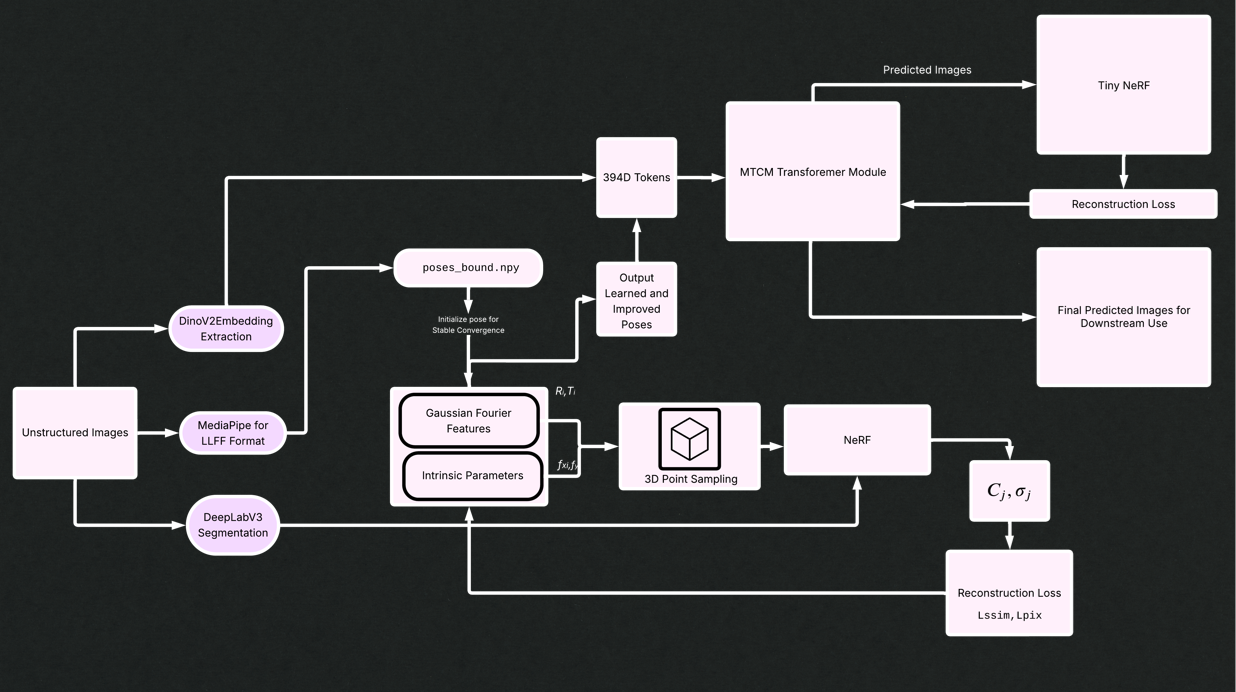
\includegraphics[width=\textwidth]{images/system2.png}
    \caption{System architecture for the integrated pose refinement and view selection pipeline. Unstructured images are preprocessed through segmentation (DeepLabV3), pose estimation (MediaPipe to LLFF format), and embedding extraction (DINOv2). Coarse poses are refined via Gaussian Fourier Features and an MLP-based regressor, supervised by a NeRF rendering loss ($\mathcal{L}_{\text{SSIM}}$, $\mathcal{L}_{\text{pix}}$). The refined poses and embeddings form 394D multimodal tokens that enter the MTCM Transformer Module, which selects optimal views. A TinyNeRF module provides reconstruction-loss supervision for the selection process, and the final predicted images are passed to the downstream reconstruction pipeline.}
    \label{fig:nerf_system_architecture}
\end{figure}


\subsubsection{Preprocessing}

The pipeline begins by converting an unstructured image collection into a structured, LLFF-compatible format enriched with semantic and geometric metadata. This stage is necessary for stable downstream optimization, especially without calibrated multi-view input.

Each image first undergoes semantic segmentation using DeepLabV3~\cite{chen2018deeplabv3} to isolate the foreground subject and generate RGBA masks. These masks improve the robustness of both pose estimation and NeRF supervision by filtering out cluttered backgrounds and occlusions.

Coarse camera extrinsics are then estimated using a hybrid method that combines MediaPipe's~\cite{mediapipe2023} facial landmark detector with OpenCV's Perspective-n-Point (PnP) solver~\cite{opencv_solvepnp}. Given 2D facial landmarks and a sparse 3D head model, the PnP solver computes initial rotation and translation vectors for each image. These estimates are stored as \texttt{poses\_bound.npy} files in COLMAP-compatible LLFF format for downstream processing, as visible in the left portion of Figure~\ref{fig:nerf_system_architecture}.

In parallel, DINOv2~\cite{dinov2_2023} extracts high-dimensional visual embeddings from each masked image. These embeddings capture visual and semantic information that is later fused with pose, resolution, and segmentation metadata to form the multimodal tokens consumed by the transformer module. By the end of preprocessing, each image is associated with a coarse pose estimate, a foreground mask, and a feature embedding.


\subsubsection{Pose and focal length refinement}
\label{sec:nerftrinsic_refinement}

The coarse poses from MediaPipe are not accurate enough for high-fidelity NeRF reconstruction. To address this, the pipeline adopts a lightweight adaptation of the NeRFtrinsic Four formulation~\cite{lin2023nerftrinsic} to refine both pose and focal length estimates.

Initial extrinsics from MediaPipe provide rough pose approximations, while focal length priors come from resolution metadata. These are passed into an MLP-based regressor that encodes camera parameters using Gaussian Fourier features. This encoding makes gradient-based learning of rotation vectors $R_i$, translation vectors $T_i$, and intrinsic parameters $f_x$, $f_y$ more stable than direct parameterization. As shown in the center of Figure~\ref{fig:nerf_system_architecture}, the Gaussian Fourier Features block and Intrinsic Parameters block feed into 3D Point Sampling, which drives the NeRF rendering used for supervision.

This module is supervised via a volumetric rendering loss computed by a NeRF model trained on the predicted poses. The system minimizes a combination of SSIM and pixel-wise reconstruction losses, $\mathcal{L}_{\text{SSIM}} + \mathcal{L}_{\text{pix}}$, which encourages accurate reprojection while regularizing the solution space. The NeRF produces per-point color $C_j$ and density $\sigma_j$ values that are volume-rendered and compared against ground-truth pixels.

A key modification relative to the original NeRFtrinsic Four architecture is that only the refined pose and focal parameters are extracted during training, rather than relying on NeRFtrinsic's own volumetric reconstructions. This decoupling reduces computational overhead and allows faster convergence during joint training with the view selection transformer. The output learned and improved poses are then forwarded to the MTCM module for view selection.


\subsubsection{Transformer-based view selection (MTCM)}
\label{sec:mtcm}

Sparse-photo reconstruction quality depends heavily on which images are selected for training. Most existing NeRF pipelines treat all inputs equally, which leads to degraded results when the input set contains occlusions, extreme poses, or redundant viewpoints. The pipeline addresses this with a Multi-Token Context Model (MTCM) that learns to rank and select optimal views.

The MTCM receives a sequence of multimodal tokens. Each token comprises a 384-dimensional DINOv2 visual embedding concatenated with a 9-dimensional geometric vector containing the 3D translation, 3D rotation (expressed as axis-angle or 6D representation), and 2D focal length. This produces a 393-dimensional token per view, optionally extended with a scalar segmentation mask area and 2D image resolution to reach 394 dimensions. These are the ``394D Tokens'' shown entering the MTCM Transformer Module in Figure~\ref{fig:nerf_system_architecture}.

These tokens are normalized and linearly projected into a latent feature space. To inject spatial inductive bias, the MTCM applies both fixed sinusoidal positional encodings and a learned directional encoding block. The directional block processes pose and focal metadata via an MLP and reintegrates the result into the embedding stream, conditioning downstream attention on camera geometry.

The model backbone is a stack of transformer encoder blocks using multi-head self-attention (MHSA). In each block, token embeddings are split into queries $Q$, keys $K$, and values $V$ through learned linear projections, divided into $h$ independent heads, and used to compute scaled dot-product attention:

\begin{equation}
    \text{Attention}(Q, K, V) = \text{softmax}\left(\frac{QK^\top}{\sqrt{d_k}}\right) V
\end{equation}

\noindent where $d_k$ is the dimension of each head. The outputs of all heads are concatenated and projected back to the latent dimension, then passed through a feed-forward MLP with GELU activation and LayerNorm. Each block includes residual connections around both the attention and MLP components.

At the final layer, a selection head maps the token embeddings to scalar logits, normalized via softmax to yield per-view selection weights. During training, the top-weighted views are selected and rendered via a lightweight TinyNeRF module (top-right of Figure~\ref{fig:nerf_system_architecture}). The rendering is compared against a held-out target view using a reconstruction loss ($\mathcal{L}_{\text{MSE}}$ or $\mathcal{L}_{\text{SSIM}}$), and gradients propagate through the entire transformer stack. This allows the model to learn view selection strategies that maximize scene renderability, pose diversity, and reconstruction quality.


\subsubsection{FDNeRF-based downstream reconstruction}
\label{sec:fdnerf}

The selected views feed a custom downstream module adapted from FDNeRF~\cite{zhang2022fdnerf}. Unlike conventional NeRF pipelines, FDNeRF incorporates dynamic-aware feature warping and attention-guided multi-view aggregation. Both of these properties matter for sparse-view 3D head reconstruction, where fine pose variation and identity preservation are important.

The architecture retains FDNeRF's CNN encoder structure, augmented with a lightweight attention mechanism that maps query rays from the target view to encoded features from reference views. The attention network processes transposed query and key tensors, reshapes them into a shared latent space, and computes feature relevance via a learnable scoring function. These attention scores modulate the aggregated volume features passed to the NeRF MLP, which improves feature fidelity and multi-view consistency. This allows the system to selectively weight high-quality or spatially consistent observations while suppressing occluded or corrupted regions.

The training follows a two-phase scheme. In the first phase, FDNeRF is pretrained on a large volume of front-facing face data from VoxCeleb~\cite{nagrani2017voxceleb}, which provides a warm start for learning basic facial geometry and appearance. After two to three thousand training images, the second phase switches to data from Meta's Multiface dataset~\cite{wuu2022multiface} and the Celebrity Face Dataset~\cite{vishesh2022celebrity}, which offer more varied viewing angles and lighting conditions. This staged approach speeds up convergence and improves generalizability across identities and lighting variations.


\subsubsection{Experimental results}

The pipeline was evaluated across multiple datasets, including a personal webcam-captured dataset, celebrity portraits from the Celebrity Face Dataset~\cite{vishesh2022celebrity}, and subjects from the Meta Multiface dataset~\cite{wuu2022multiface}. All FDNeRF experiments were conducted on an NVIDIA A100 80GB GPU over approximately 10 hours of training.

\paragraph{View selection and data collection comparison.} Figure~\ref{fig:mtcm_selection_comparison} compares MTCM selection weight distributions between webcam-captured data and user-uploaded images for the same subject. The webcam-captured dataset (Figure~\ref{fig:mtcm_selection_comparison}a) exhibits tightly clustered, high selection weights, all above 0.85, indicating uniform informativeness and consistent framing across views. Even the non-selected views (red) maintain relatively high weights, reflecting the overall quality of guided capture. In contrast, the uploaded image set (Figure~\ref{fig:mtcm_selection_comparison}b) shows a broader spread in selection weights, with the top views reaching about 0.06 and a clear drop-off into a long tail of lower-weighted views. The selected views (green) are more sharply differentiated from the rejected views (red) because the MTCM must work harder to separate useful images from noisy or redundant ones. This difference confirms that guided capture via the custom web interface yields more stable inputs for downstream reconstruction.

\begin{figure}[H]
    \centering
    \begin{subfigure}[t]{0.48\textwidth}
        \centering
        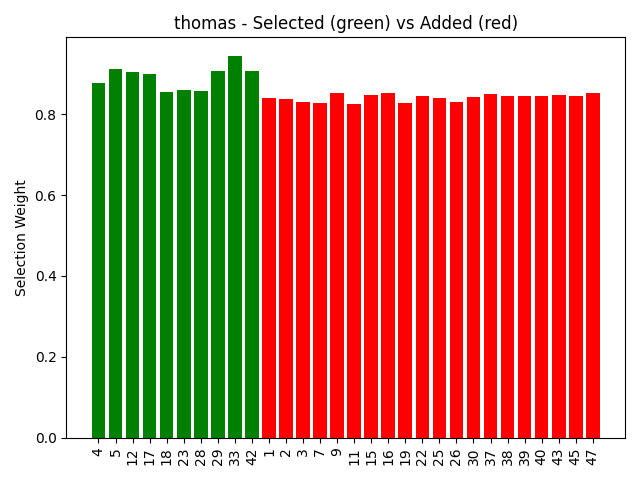
\includegraphics[width=\textwidth]{images/thomas_4_highlighted (1).png}
        \caption{Webcam-captured dataset. Selection weights are tightly clustered above 0.85 for all views, with selected views (green) marginally higher than added views (red).}
    \end{subfigure}
    \hfill
    \begin{subfigure}[t]{0.48\textwidth}
        \centering
        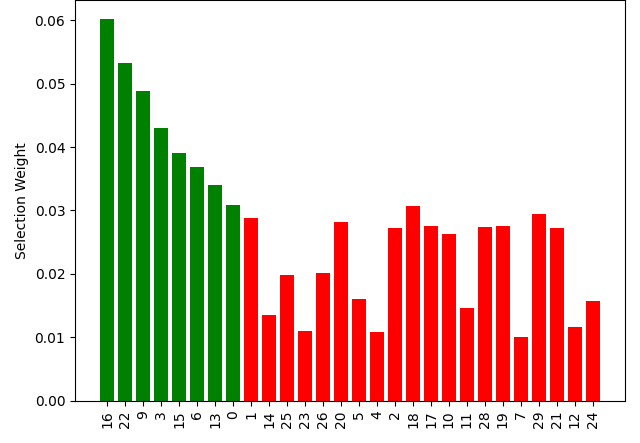
\includegraphics[width=\textwidth]{images/Thomas_4_highlighted.png}
        \caption{User-uploaded image dataset. Selection weights show a wider spread with a steeper ranking curve between selected (green) and rejected (red) views.}
    \end{subfigure}
    \caption{Comparison of MTCM selection weights across different data sources for the same subject. (a)~Structured webcam-captured data yields uniformly high weights, reflecting consistent quality from guided capture. (b)~Unstructured uploaded images produce more differentiated selection patterns, confirming the benefits of guided capture for reliable view selection.}
    \label{fig:mtcm_selection_comparison}
\end{figure}

\paragraph{FDNeRF reconstruction quality.} Figure~\ref{fig:fdnerf_reconstruction} shows a representative FDNeRF reconstruction result at epoch 2000. The leftmost images are the MTCM-selected input views after segmentation and background removal, showing the subject from a range of angles. The second-to-last image shows the volumetric density field learned by the network, a blue-tinted visualization of the 3D structure the model has internalized. The rightmost image is the final rendered output at the held-out target view, achieving a PSNR of 17.587~dB. The result preserves recognizable identity features such as facial structure, glasses, and hair, despite being reconstructed from only a handful of sparse, casually captured views. The density field visualization confirms that the network has learned a coherent 3D structure rather than simply memorizing 2D appearance.

\begin{figure}[H]
    \centering
    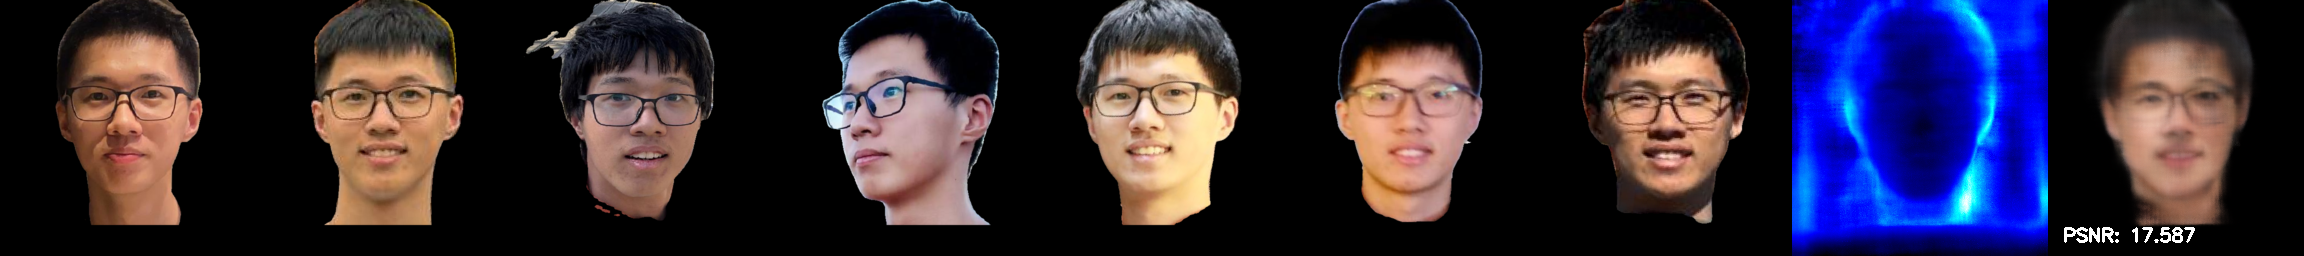
\includegraphics[width=\textwidth]{images/0008_2000_vis.png}
    \caption{FDNeRF reconstruction result at epoch 2000 using MTCM-selected views. From left to right: the selected input views after segmentation and background removal (showing diverse head angles), the learned volumetric density field (blue visualization), and the final rendered output (PSNR: 17.587~dB).}
    \label{fig:fdnerf_reconstruction}
\end{figure}

\paragraph{Novel view synthesis.} Figure~\ref{fig:novel_view_synthesis} shows two novel viewpoints rendered from the same trained model, confirming that the reconstruction generalizes beyond the input views. In the three-quarter view (Figure~\ref{fig:novel_view_synthesis}a), facial features, glasses, and skin texture are preserved with reasonable fidelity despite this viewpoint not being present in the original input set. The side profile (Figure~\ref{fig:novel_view_synthesis}b) shows that the ear, jawline, and hair volume remain geometrically consistent, which confirms that the reconstructed radiance field encodes plausible 3D structure rather than view-dependent appearance alone.

\begin{figure}[H]
    \centering
    \begin{subfigure}[t]{0.48\textwidth}
        \centering
        
\includegraphics[width=\textwidth]{images/1.png}
        \caption{Three-quarter view rendering from a novel camera trajectory. Facial features, glasses, and skin texture are preserved despite this viewpoint not being present in the original input set.}
    \end{subfigure}
    \hfill
    \begin{subfigure}[t]{0.48\textwidth}
        \centering
        
\includegraphics[width=\textwidth]{images/2.png}
        \caption{Side-profile rendering under camera motion. The ear, jawline, and hair volume remain geometrically consistent, confirming plausible 3D structure in the reconstructed radiance field.}
    \end{subfigure}
    \caption{Novel view synthesis results from FDNeRF trained with MTCM-selected views captured through the custom web interface. Both renders show viewpoints not present in the original input images.}
    \label{fig:novel_view_synthesis}
\end{figure}


\subsubsection{Mesh extraction, relighting, and texture synthesis}

3D meshes were extracted from FDNeRF outputs by applying the Marching Cubes algorithm on the predicted signed distance field. RGB textures were applied using UV maps derived from xatlas. These meshes were then passed through a relighting module implemented in Blender. A custom automation toolkit, consisting of Python scripts for camera orbit paths and lighting presets, simulates a range of lighting conditions. The toolkit exposes parameters for lighting mode, HDRI usage, and animation duration, and supports volumetric fog, HDRI environment rotation, and frame-accurate lighting transitions.

Figure~\ref{fig:mesh_and_relighting} shows the full progression from extracted mesh to relit output. The base mesh (Figure~\ref{fig:mesh_and_relighting}a) is loaded in Blender with the scene outliner showing the mesh object alongside a camera and light. The Transform panel confirms position and scale. The reconstruction captures head shape, hair geometry, glasses, and clothing, though some noise is visible at the top of the head where Marching Cubes produced incomplete surfaces at the volume boundary. Figures~\ref{fig:mesh_and_relighting}b and~\ref{fig:mesh_and_relighting}c show the same mesh under two cinematic lighting presets from the custom Interactive Lighting panel. The Film Noir setup uses a three-light rig (Noir\_Edge, Noir\_Fill, Noir\_Key) with deep shadows and high contrast. The Sci-Fi setup uses colored rim lights (SciFi\_Key, SciFi\_Rim1, SciFi\_Rim2), producing a green-and-magenta stylized look. The Interactive Lighting panel, visible in both screenshots, also lists Three Point Lighting and Sunset Lighting as additional one-click presets. That the same mesh responds plausibly to such different lighting conditions suggests sufficient geometric and texture fidelity for downstream rendering tasks.

\begin{figure}[H]
    \centering
    \begin{subfigure}[t]{0.32\textwidth}
        \centering
        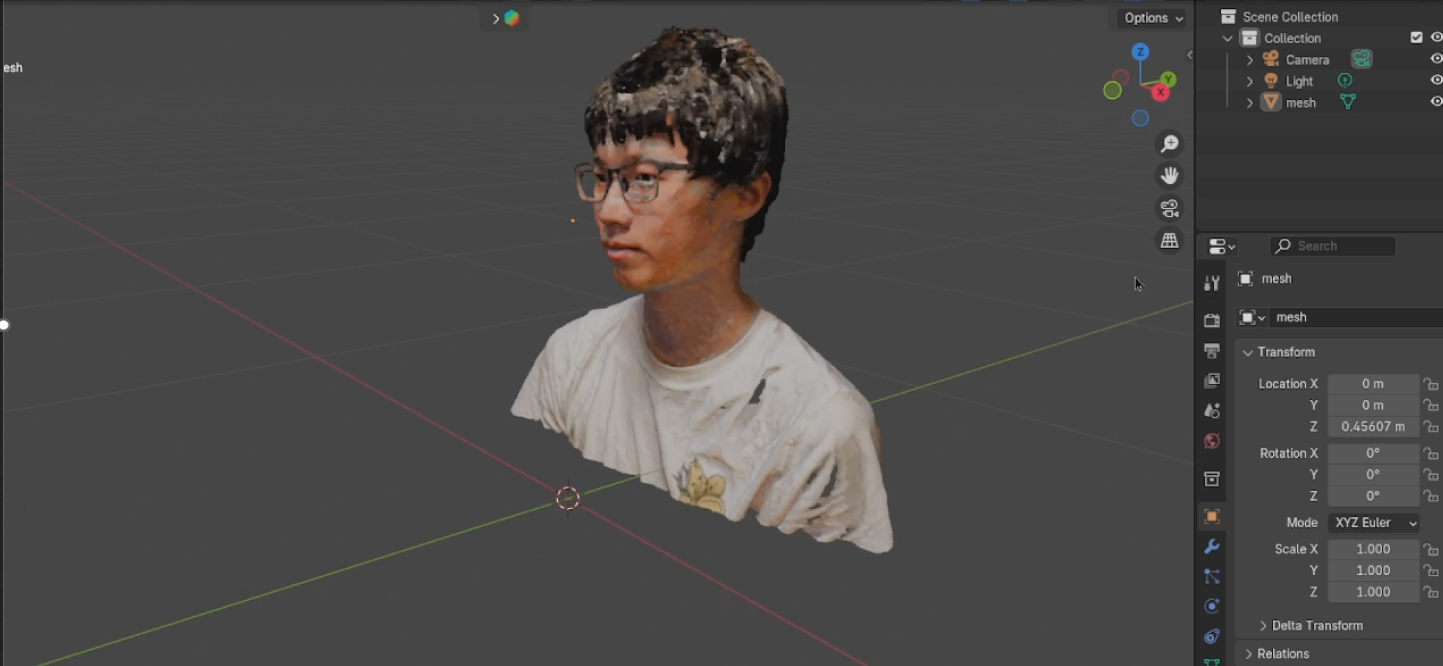
\includegraphics[width=\textwidth]{images/4.png}
        \caption{Textured 3D mesh in Blender after Marching Cubes extraction and xatlas UV unwrapping. The outliner and Transform panel are visible on the right.}
    \end{subfigure}
    \hfill
    \begin{subfigure}[t]{0.32\textwidth}
        \centering
        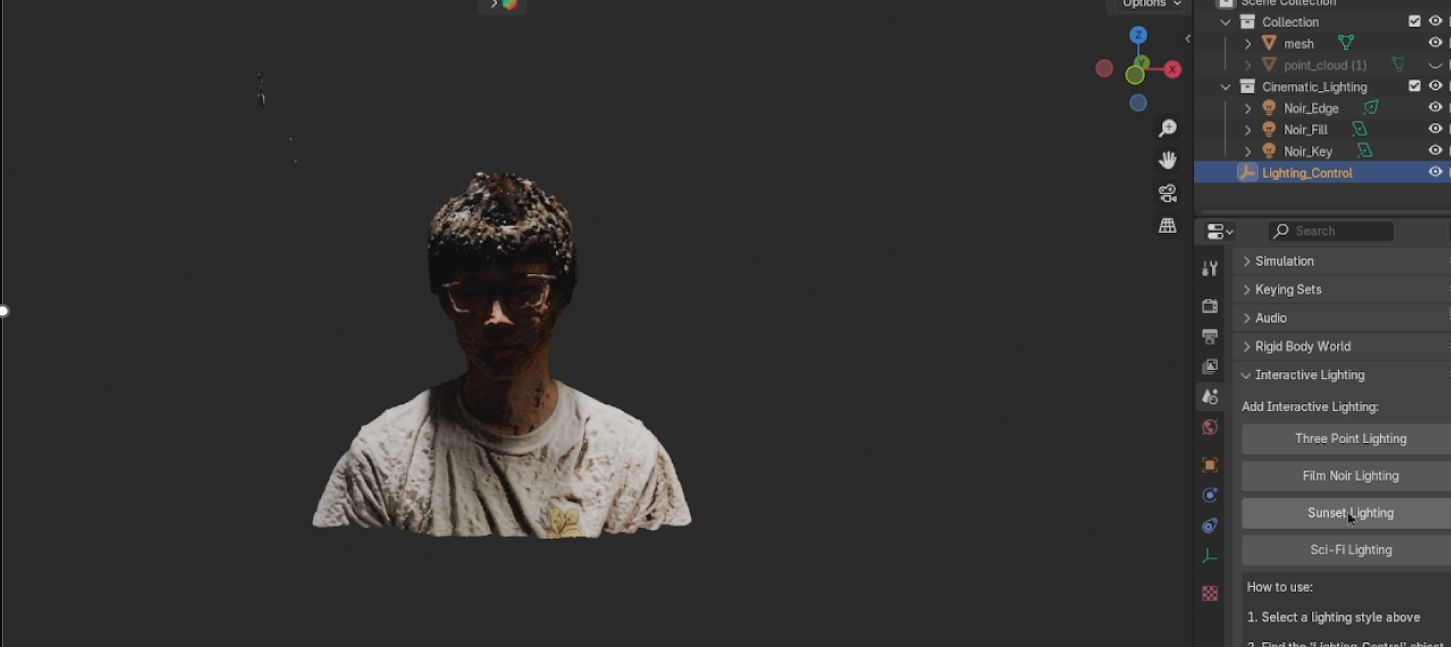
\includegraphics[width=\textwidth]{images/5.png}
        \caption{Film Noir lighting preset. The Noir key, fill, and edge lights produce high-contrast directional illumination with deep shadows.}
    \end{subfigure}
    \hfill
    \begin{subfigure}[t]{0.32\textwidth}
        \centering
        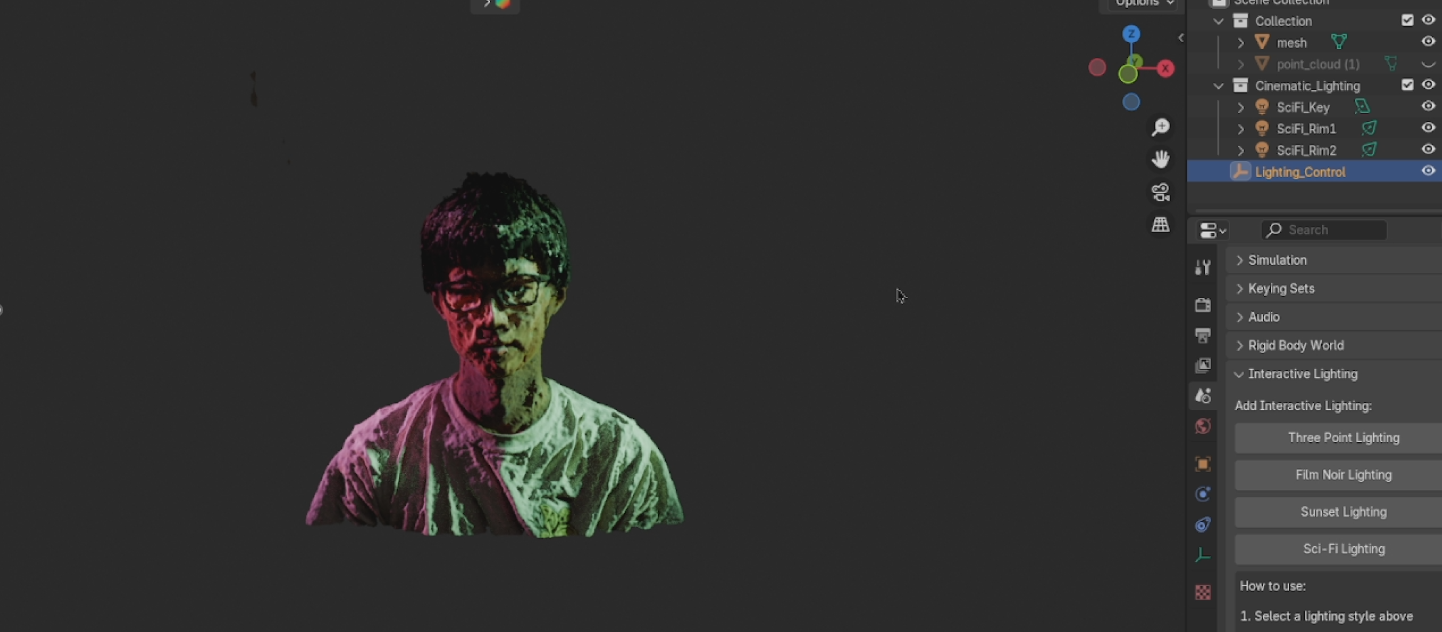
\includegraphics[width=\textwidth]{images/6.png}
        \caption{Sci-Fi lighting preset with colored rim lights (SciFi\_Key, SciFi\_Rim1, SciFi\_Rim2), producing stylized green-and-magenta illumination.}
    \end{subfigure}
    \caption{Mesh extraction and relighting results. (a)~The base textured mesh extracted via Marching Cubes from FDNeRF's signed distance field. (b,\,c)~The same mesh rendered under two cinematic presets from the scripted Blender lighting controller.}
    \label{fig:mesh_and_relighting}
\end{figure}


\subsubsection{Web-based data collection interface}

To reduce pose noise from uncontrolled captures, a custom web-based data collection interface was developed (Figure~\ref{fig:web_interface}). The tool provides two input modes: Webcam Capture for guided multi-pose recording, and Upload Files for existing photographs from smartphones or other cameras. In webcam mode, the interface prompts users to rotate their heads in multiple directions while capturing frames automatically. In both cases, the interface performs segmentation and metadata extraction in real time.

Although the resulting images remain unstructured in the NeRF sense, with no calibrated camera rig, their improved framing and pose diversity lead to higher-quality initial estimates than ad-hoc photo collections. From these captures, the top 8 images are selected by MTCM for final rendering, while the remaining 40 to 50 frames are used to pretrain FDNeRF in the first phase of the two-stage training scheme. The comparison in Figure~\ref{fig:mtcm_selection_comparison} confirms the value of this guided capture approach: webcam-captured data consistently produces higher and more uniform MTCM selection weights than unstructured uploaded images of the same subject.

\begin{figure}[H]
    \centering
    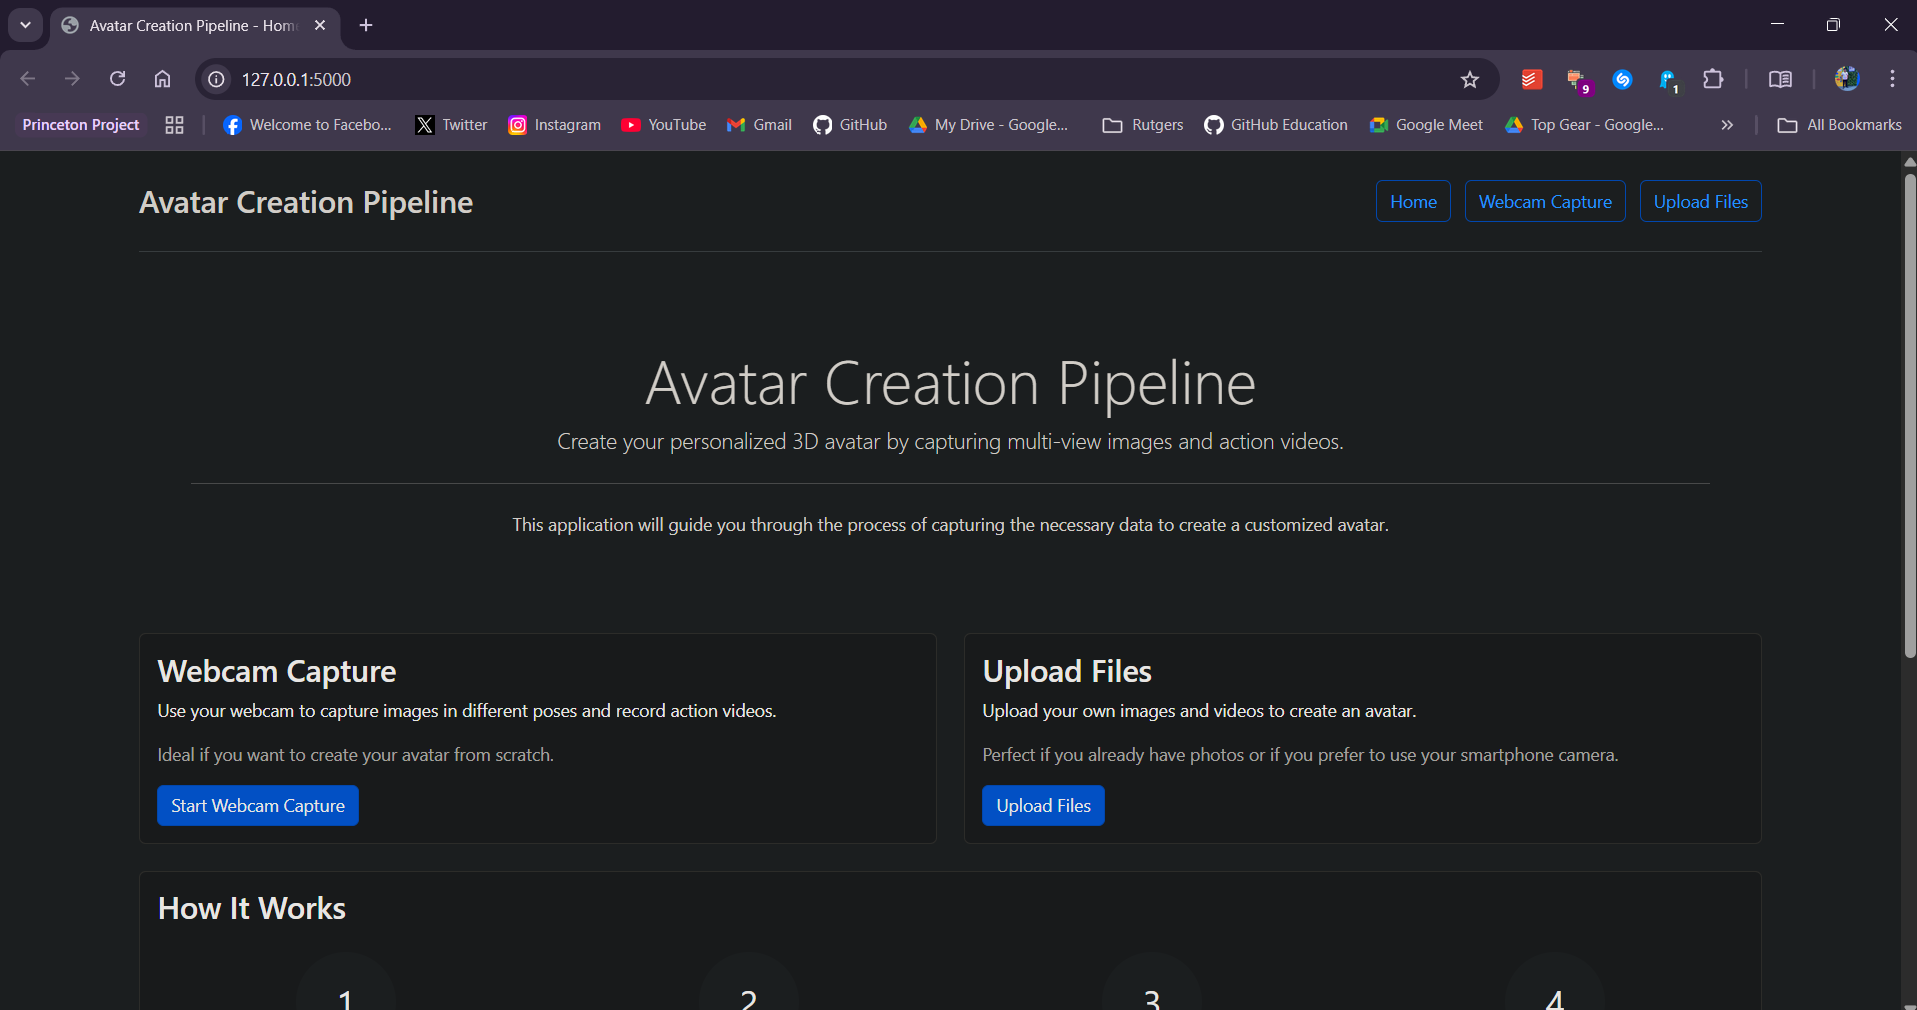
\includegraphics[width=0.75\textwidth]{images/7.png}
    \caption{The custom-built web interface for image capture and avatar generation. The landing page offers Webcam Capture and Upload Files modes, with a ``How It Works'' guide below. The interface runs locally and triggers the segmentation and pose prediction pipeline automatically upon submission.}
    \label{fig:web_interface}
\end{figure}


\subsubsection{Engine-facing future integration}

The next step is to convert this reconstruction pipeline into an engine-facing workflow. In practical terms, that means taking the outputs of the avatar pipeline and mapping them into a representation suitable for runtime use, including geometry, textures, material definitions, and attachment points for animation or interaction. This is where the present gap lies. Reconstruction has been explored, but a robust bridge to import, asset validation, rigging compatibility, and runtime rendering still needs to be built.

A useful future architecture would treat the NeRF system as an offline or semi-offline asset-generation stage, followed by a conversion pipeline that prepares scene-ready outputs for LAGEngine. This would preserve the strengths of neural reconstruction without forcing the core engine runtime to depend on an expensive neural rendering loop. It would also make it easier to expose this feature through the editor in a way that remains practical for classroom use, so that a student can generate their own avatar from a short image capture session and drop it into a running simulation with minimal friction.

{\footnotesize
\bibliographystyle{IEEEtran}
\bibliography{references}
}
\end{document}